\documentclass[a4paper,10pt]{article}
\usepackage[utf8]{inputenc}
\usepackage{latexsym}
\usepackage{amsmath}
\usepackage{amsthm}
\usepackage{amsfonts}
\usepackage{enumerate}
\usepackage{color}
\usepackage{listings}
\usepackage{todonotes}
\usepackage{placeins}
\lstset{basicstyle=\ttfamily,language=Python}

\title{PoC internal report}
\author{The Aleph Zero team}
\begin{document}
 \maketitle
	This is the internal report from the final round of tests we ran on the proof-of-concept implementation of the Aleph protocol.
	The implementation is written in Python and can be accessed at \todo[inline]{Make a tag and link it here.}.
	\section{General setup}
	This sections gives an overview of the main experimental setup.
		\subsection{Settings}
			We experimented with various constants than can be set in the implementation. Short descriptions of them follow.
			\begin{description}
				\item[create delay] The minimum amount of time, in seconds, to wait between finishing a unit and initiating the creation of a new one. Values are $.5$, $1$, and $2$.
				\item[sync delay] The minimum amount of time, in seconds, to wait between initiating a sync and initiating another one. Values are between $.015625$ and $.25$, doubling each step.
				\item[committee size] The number of processes in the committee. Values are $32$, $64$, $128$, $256$ and $512$.
				\item[transactions per unit] The number of transactions included in a single unit. Values are $1$, $100$, and $1000$.
				\item[maximum number of parents] The maximal number of parents a unit can have. Values are $10$, $20$ and $128$, the latter simulating a lack of limit.
				\item[maximum number of incoming/outgoing syncs] The maximal number of incoming and outgoing syncs happening at the same time.
					These are separate constants but in our tests they share the same value. Values are $10$ and $32$.
			\end{description}
		\subsection{Main values}
			The core values in the results are outlined below.
			\begin{description}
				\item[latency] How long it took for a newly created unit to be validated. Perhaps the most important number.
				\item[transactions per second] How many transactions were introduced into the system every second.
				\item[sync delay] How long it actually took to initiate a new sync after the previous one. Important for assessing whether the processes ``keep up''.
				\item[create delay] How long it actually took to initiate a new unit creation after the previous one. Important for assessing whether the processes ``keep up''.
				\item[number of parents] How many parents did a unit have. Important for assessing whether the processes have enough information when creating units.
			\end{description}
	\section{Algorithms}
		A single process does many things:
		\begin{itemize}
			\item Creating units.
			\item Adding units to the poset.
			\item Sending and receiving units.
			\item Computing decisions for timing units.
		\end{itemize}
		A short description of the algorithms involved and their complexity follows.
		\subsection{Expensive operations}
		 Before we detail the algorithms we point out several important optimization details that we will refer to in further parts of this section.
			For purposes of complexity estimation let $N$ denote the number of processes in the committee and $p$ the number of parents a single unit has.
			The latter might vary per unit, but we usually have an upper bound.

			The most important feature of the poset we maintain in the algorithm is of course its order.
			For comparing units we use the \lstinline{below} method. In the absence of forks (which is the case in all the tests) this method works in constant time.
			This, however, requires maintaining a helper structure in every unit $U$ called \lstinline{floor}.
			This structure is a list of lists, a list at position $k$ contains the maximal units made by process $k$ that are below $U$.
			To check whether $V$ is below $U$ we check if \lstinline{U.floor[V.creator_id][0].height >= V.height}.
			Maintaining \lstinline{floor} requires more work. When adding a unit to the poset we combine the floors of its parents.
			This operation runs in $O(N*p)$ time and is one of the more expensive ones.
		\subsection{Creating units}
		 \label{sec:creation}
			The most expensive part of creating a unit $U$ is choosing its parents. Because of historical reasons we do this somewhat suboptimally.
			We set the first parent to the last unit created by the process creating $U$. Every subsequent parent we choose as follows.
			A list is created by taking all the maximal units of the poset and finding the ones which \emph{do not} satisfy the expand primes rule (described in section \ref{sec:adding}).
			We then take the list of maximal units and remove the members of the previous list and all the previous parents.
			We choose a random unit from this list and add it as a parent. This is repeated until we either cannot add any more parents or reach the limit of parents.

			Checking whether a unit satisfies the expand primes rule takes $O(N)$ time and we have to do this for at most $N$ units.
			The whole process is repeated $p$ times, giving us a final time of $O(N^2*p)$.
			This is relatively slow, but it is worth pointing out that creation happens relatively rarely, so it shouldn't have big effects on the overall run time.

			After initial tests another, more efficient, algorithm for choosing parents was implemented.
			We first pick all maximal units of maximal level in the poset, ones that were added latest first.
			Then we add them greedily as parents as long as they satisfy the expand primes rule.
			Afterwards we check maximal units of level equal to the predecessor's level and if they could be added before the previously chosen parents.
			Once again we choose greedily and add as much as is legal. The whole process only takes $O(N*p)$ time.
			These two steps more or less correspond to the two requirements on optimal poset structure, see Section \ref{ssec:posetShape}.
		\subsection{Adding units to the poset}
		 \label{sec:adding}
		 Adding units to the poset consists of several potentially computationally expensive steps:
			\begin{enumerate}
				\item Checking unit compliance.
				\item Computing the level of a unit.
			\end{enumerate}

			Compliance checking consists of multiple parts, but in this document we restrict the discussion to the ones that might be computationally expensive.
			For a more through list of steps see the \lstinline{check_compliance} documentation.
			\begin{enumerate}
				\item We check whether the unit proves that its creator produced a fork. This requires combining floors, which takes $O(N*p)$ time.
				\item We check whether any of its parents proves that the creator of any other parent is a forker. This takes $O(p^2)$ time,
					because the parents are already in the poset, so no floor combining is needed.
				\item We check whether the ``expand primes'' rule is satisfied. This should take (as described below) at most $O(N*p)$ time.
			\end{enumerate}
			All in all compliance should take about $O(N*p)$ time, which at worst can degenerate to $O(N^2)$ if we don't restrict the number of parents.

			The ``expand primes'' rule means that every parent after the first has to satisfy one of the conditions:
			\begin{itemize}
				\item Have level greater than the previous one.
				\item Be above more prime units of level equal to the previous parent's level, than all the previous parents combined.
			\end{itemize}
			Checking the former condition requires constant time, but the latter requires iterating over at most all prime units of the specified level.
			Since we do it for every parent this takes $O(N*p)$ time, as asserted above.

			Computing the level consists of iterating over all prime units of the level of the unit's predecessor and checking whether a sufficient number of them is below the unit.
			It takes only about $O(N)$ time, but if the number of parents is restricted this is comparable to compliance checking.
		\subsection{Sending and receiving units}
		 Determining which units to send only takes time linear with respect to the number of units that actually have to be sent.
			Then we have to order the units topologically -- we do this before sending them, but it has to be done at some point so there is no time to be saved here.
			This takes at most $O(k*p)$ time, where $k$ is the number of units to send.

			This is mostly relevant when $k$ is big, i.e. when the processes syncing are significantly desynchronised.
			This sometimes happens in our tests, because the machines don't start at once.
			However after a while the effects are negligible.
		\subsection{Computing decisions for timing units}
		 The most time expensive part of timing decisions is checking for popularity proofs.
			To check if a unit proves the popularity of another we traverse the poset graph between the two units and check whether
			we encounter units created by sufficiently many processes. This takes time linear with the number of edges encountered,
			which is $p$, times the number of units encountered. This is only ran between units differing by $3$ levels, so the number of units
			is about $3*N*t$, where $t$ is the average number of units created by a single process at a single level (the ``thickness'' of a level).
			It is worth pointing out that in many of our experiments	$t = 1$.

			The attempt at proving popularity can be ran for up to $N$ unit consecutively, so this single operation can take $O(N*N*p*t)$ time.
			When $p$ is close to $N$ this turns into $O(N^3*t)$, which is much more expensive than any other single operation we use.
			However, we memoize the results, so this should only happen very infrequently, at most for one unit per level in the whole poset.

			Other methods relating to timing decisions take about $O(N)$ time, so much faster.
	\section{Known bottlenecks}
		The main thing to note before we begin discussing bottlenecks is what we are actually trying to optimise.
		Running time of specific operations is not particularly important to us, what we care about is mostly the latency,
		i.e. how much time passes between a unit being added to the poset and it being included in the linear order.
		Due to that the structure of the poset that our algorithm builds might often be more important than how long various operations take.

		Another important point is that every CPython program has a singular event log, which is completely synchronous, so it cannot run anything in a truly separate thread.
		Due to that, even though the code is written in an ``asynchronous'' manner, any CPU intensive operation will block everything until it completes.
		It can, however, run network operations, like waiting for sending/receiving data, in the background by deferring them to the OS.

		This brings us to our first and most obvious bottleneck, network operations.
		\subsection{Network capacity and latency}
			During the execution of our algorithm we have to send quite big amounts of data through the network.
			In a rough overview our sync protocol has the following steps:
			\begin{enumerate}
				\item Initiate the sync by sending the state of our poset in the form of heights and hashes of maximal units per process.
				\item Receive similar information from the other process, followed by units it inferred we don't know about.
				\item Send the units we infer the other process doesn't know about.
			\end{enumerate}
			This description omits anything related to fork handling, as those are not present in the tests.
			The full protocol can be found in the documentation of \lstinline{aleph.network}.

			Because of these operations being almost properly parallelized it is hard to tell how much of a bottleneck they really are.
			We expect that sending many units through the network can take a long time, so if two processes are heavily desynchronised this might be noticeable.
			However, in such cases adding the units takes a significant amount of time and is probably a bigger bottleneck.
		\subsection{Adding units}
			As detailed in Section \ref{sec:adding} adding units after a sync can take a significant amount of time if the processes are sufficiently desynchronised.
			Because of the way parallelism is handled in Python this can block for a long time and delay crucial operations such as unit creation and syncing.
			Such desynchronisation should only occur at the start of experiments, when some machines begin participating in the algorithm much later than others.
			However, this problem might cause a vicious circle, by causing delays sufficient to desynchronise processes again.
			This might be the case in some of the most intensive tests.
		\subsection{Poset structure}
		 \label{ssec:posetShape}
			As mentioned at the beginning of this section the structure of the poset has immense influence over the final validation latency.
			There are two crucial components influencing this speed:
			\begin{enumerate}
				\item Thickness of a level, i.e. how many units made by a process were at that level.
				\item How quickly units become popular, i.e. how quickly they are below units made by $2/3$ of the processes.
			\end{enumerate}
			The former should be as low as possible, because a unit can only be included in a linear order after at least three levels are build on top of it.
			Since we limit how often new units are created, making level unnecessarily thick wastes time.

			The latter should be as quick as possible, because when a unit is being considered for a timing unit its popularity determines how many levels it will take to decide.
		 Therefore, we are once again bound by rate limiting unit creation.

			The results were best for posets in which most levels had thickness $1$ (one unit per process at every level) and almost every unit was popular very quickly.
	\section{Results}
	 We ran 3 big series of experiments. After each set we noticed and fixed problems in code, so unfortunately the runs are not directly comparable.
		However their results should still give a good intuition with regards to the Aleph protocol.
		\subsection{Delays}
		\FloatBarrier
			The first series of experiments was testing various values of create and sync delays.
			In all tests the committee size was $128$, there was $1$ transaction per unit, maximally $10$ parents, and $10$ simultaneous incoming/outgoing syncs.
			The values of create and sync delays can be seen in the graphs.
			It is worth pointing out that one of the tests had a create delay of $.1$ as a stress test.
			\begin{figure}[h]
				\centering
				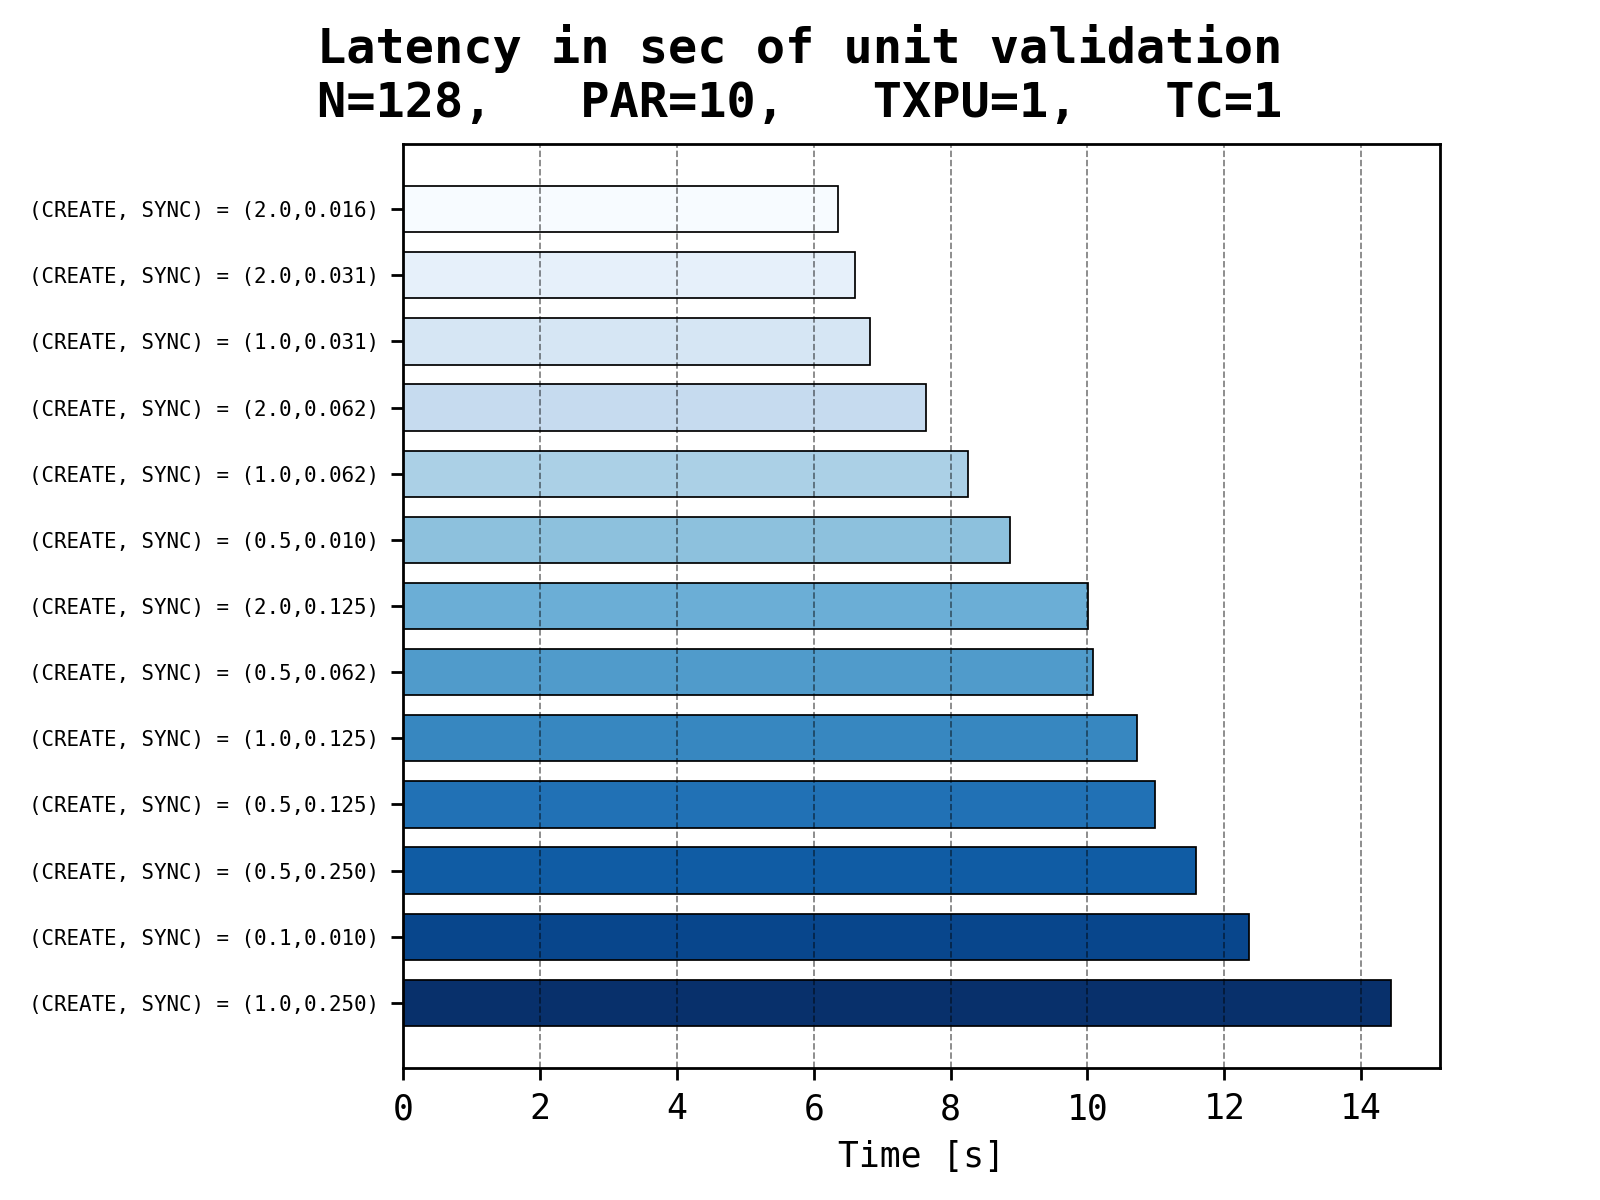
\includegraphics[width=0.8\textwidth]{bar_plots/final_exp1/create_ord_del.png}
				\caption{The latency of unit validation in the first series of experiments.}
				\label{fig:delaysLatency}
			\end{figure}
			\begin{figure}[h]
				\centering
				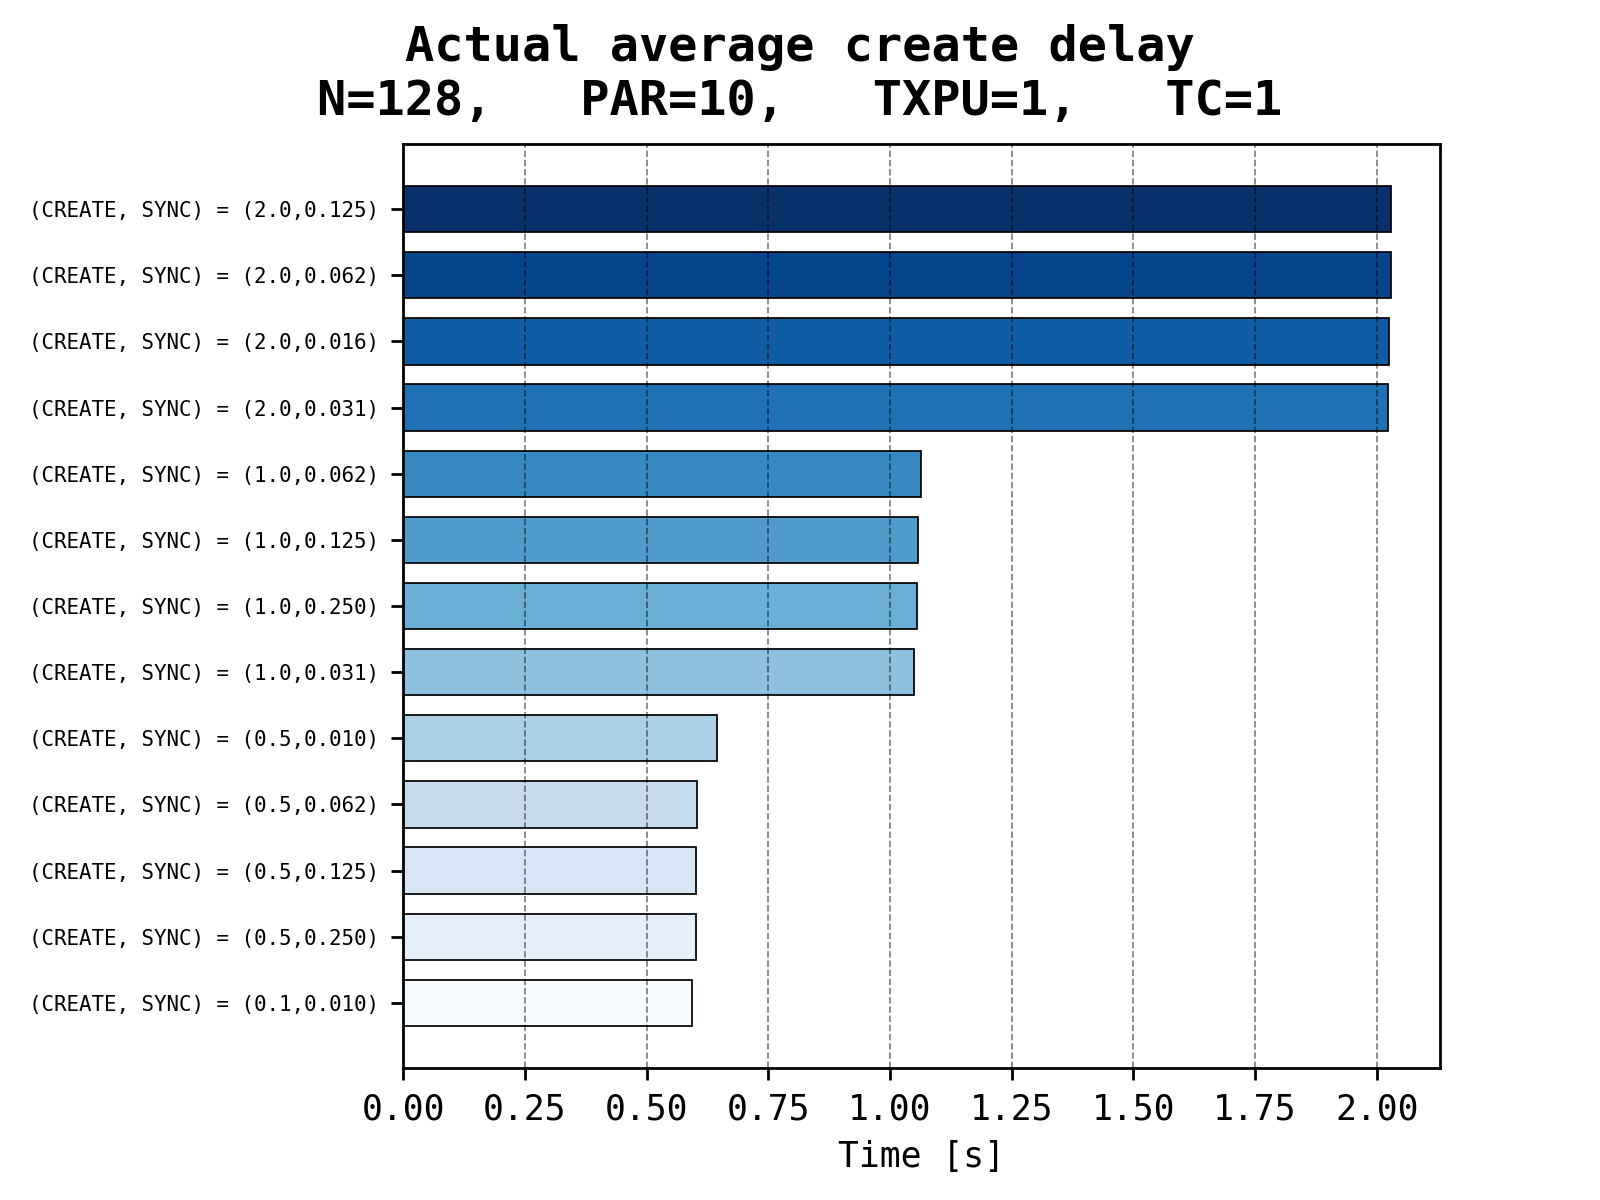
\includegraphics[width=0.8\textwidth]{bar_plots/final_exp1/create_delay.png}
				\caption{The time between unit creation attempts. Note that in the case of $.1$ delay this is not much different than $.5$.}
				\label{fig:delaysCreateDelay}
			\end{figure}
			\begin{figure}[h]
				\centering
				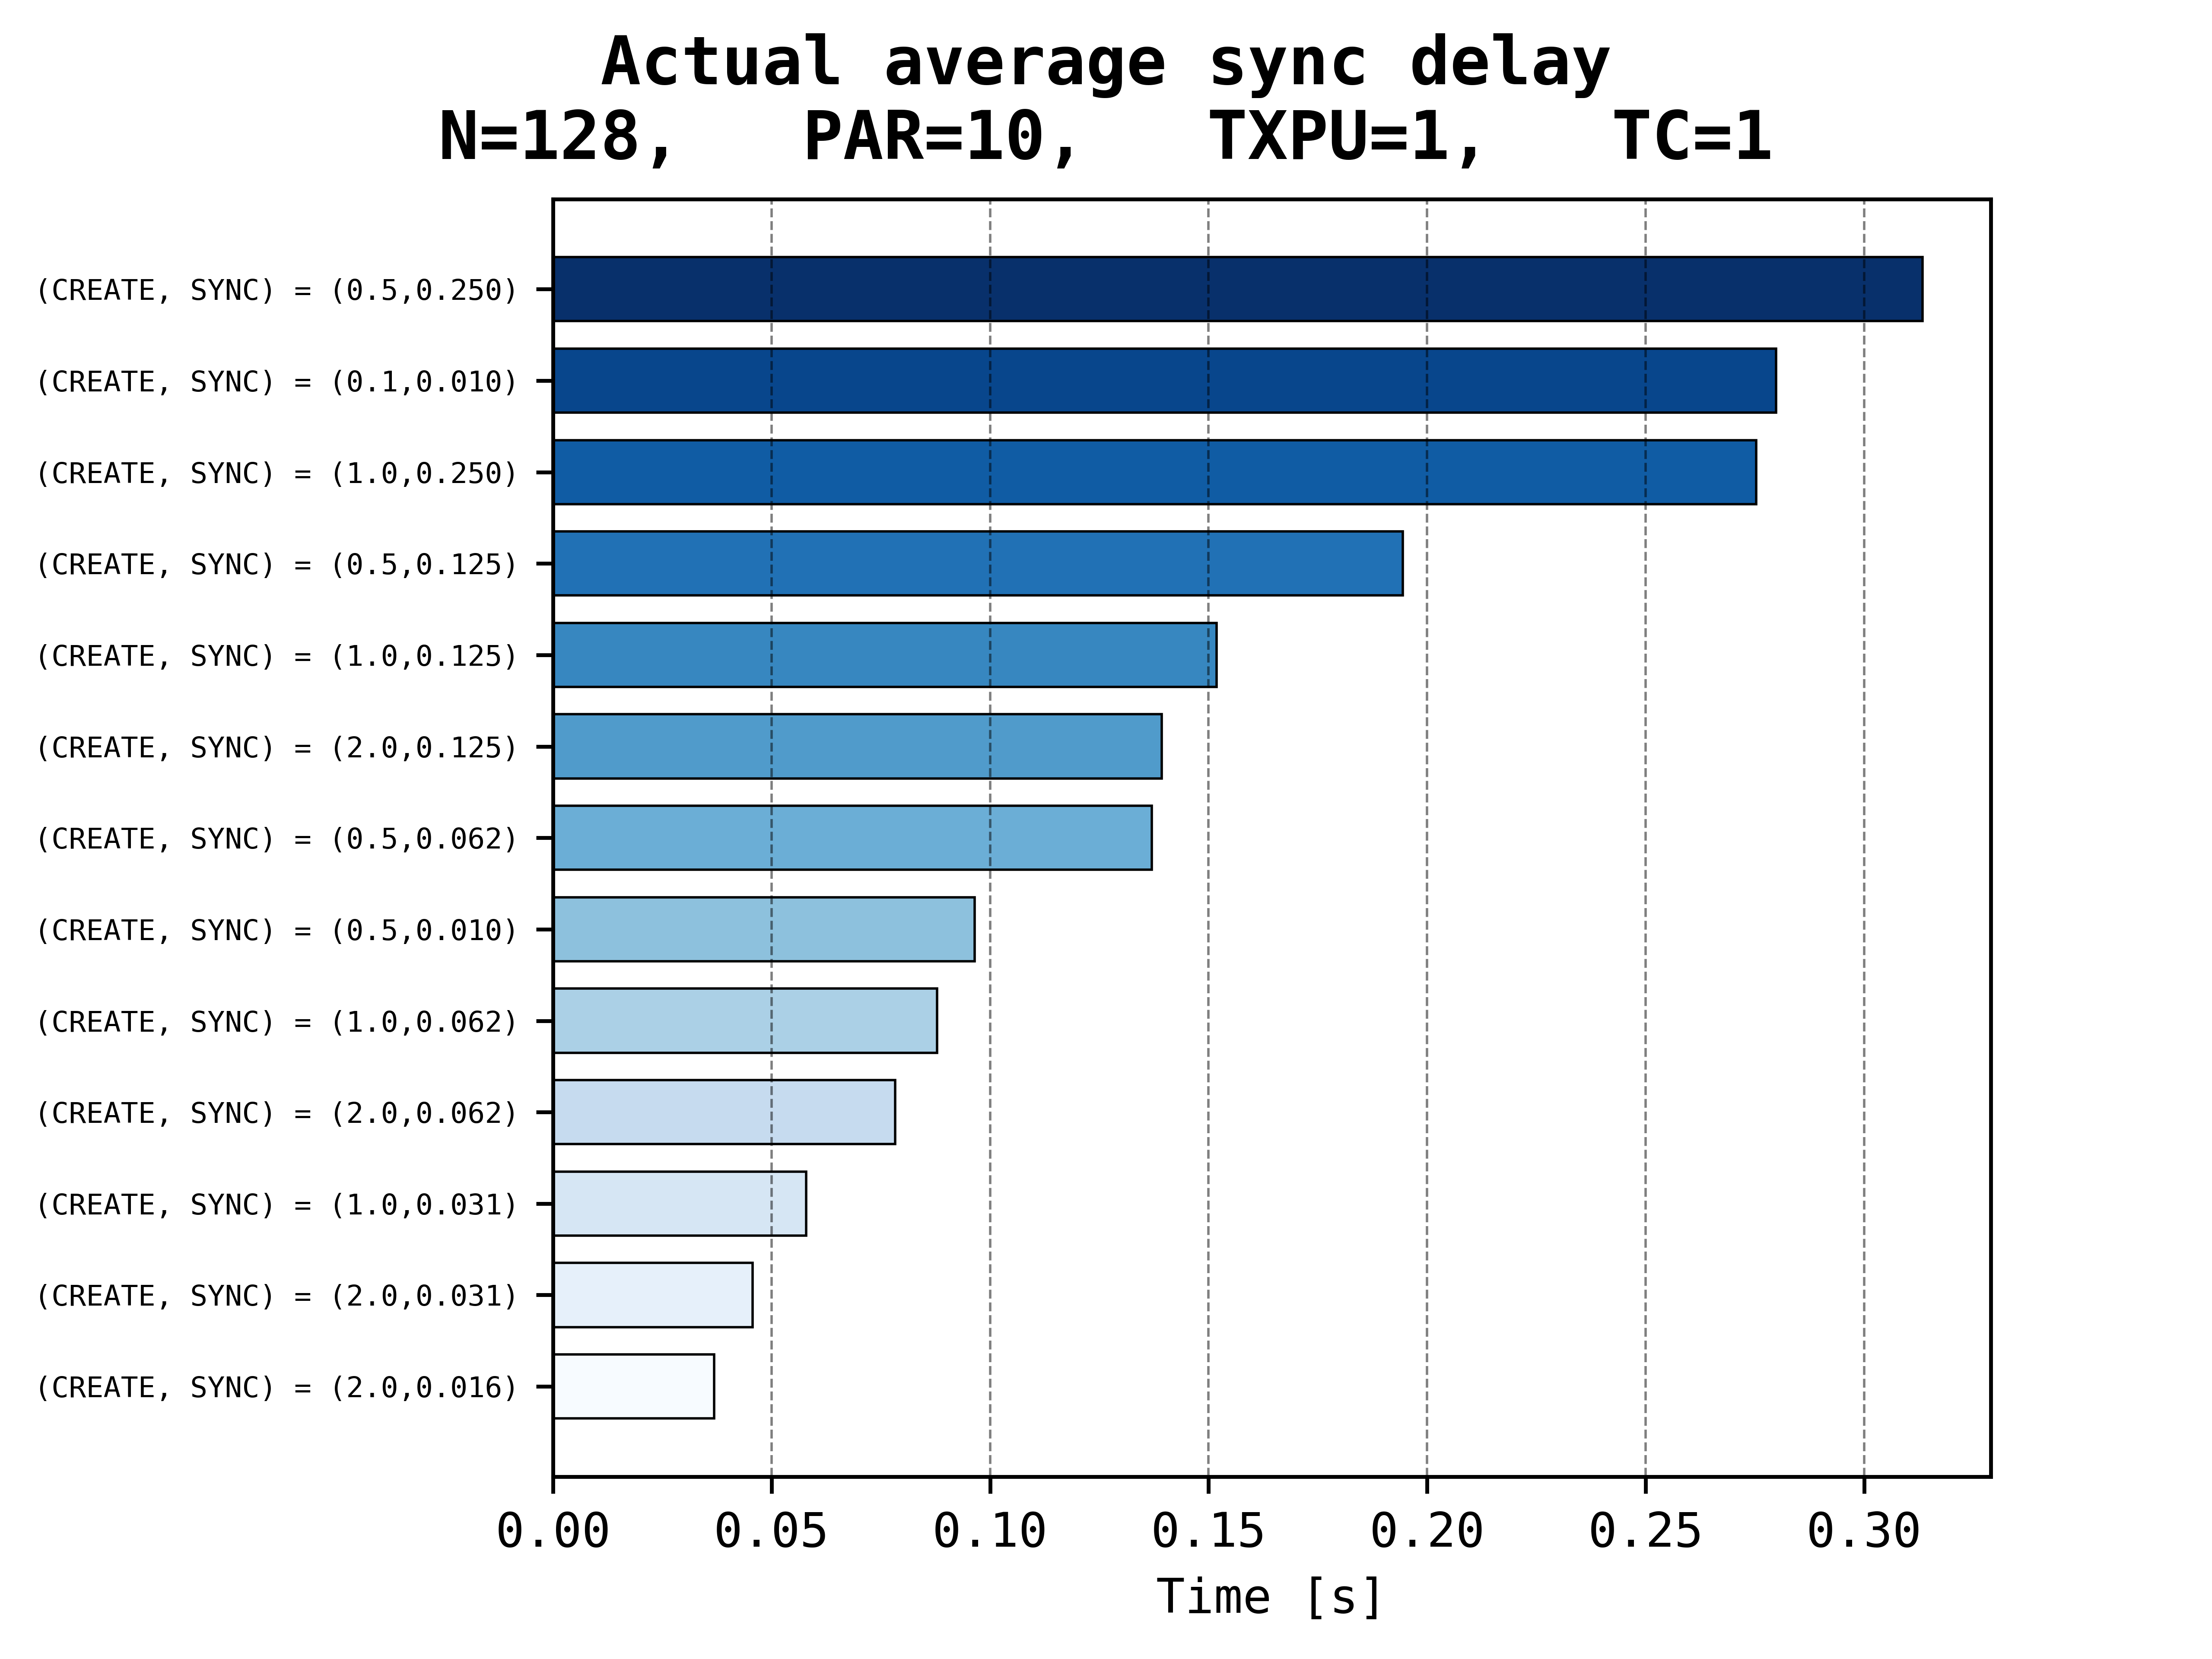
\includegraphics[width=0.8\textwidth]{bar_plots/final_exp1/sync_delay.png}
				\caption{The time between sync attempts. Note that this is often much bigger than the sync delay would suggest.}
				\label{fig:delaysSyncDelay}
			\end{figure}
			\begin{figure}[h]
				\centering
				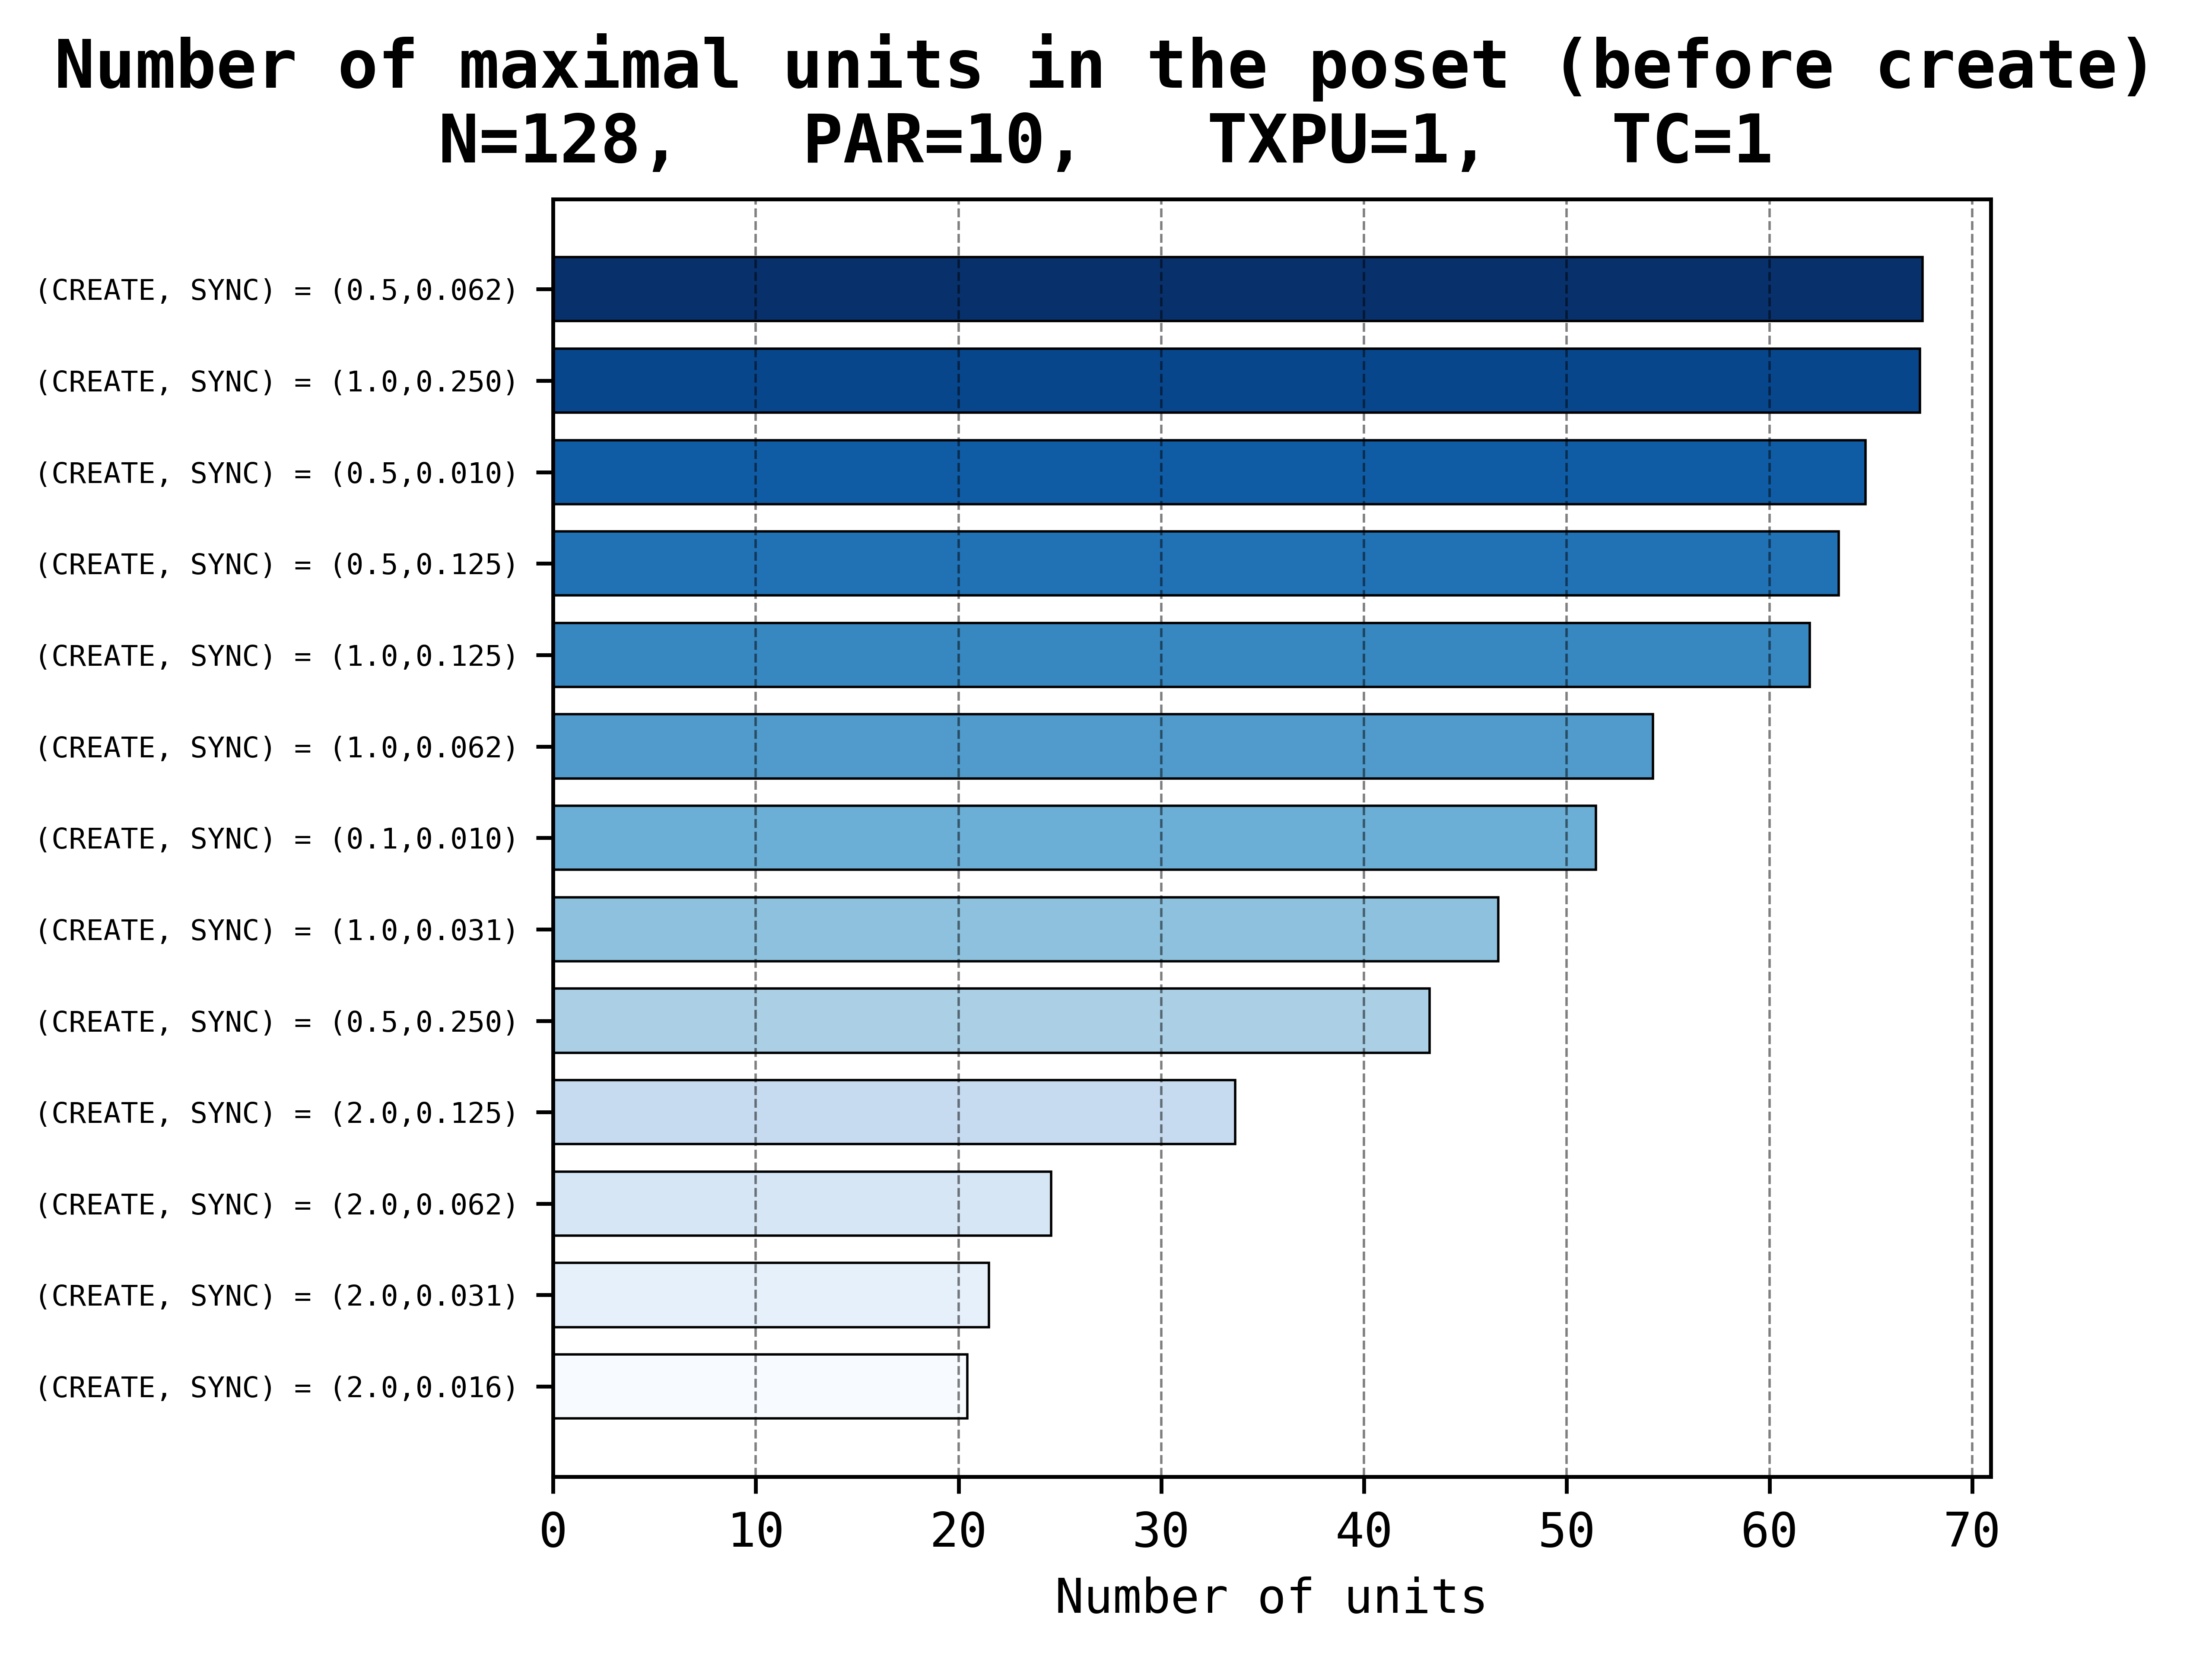
\includegraphics[width=0.8\textwidth]{bar_plots/final_exp1/n_maximal.png}
				\caption{Number of maximal units in the poset before a create, this is also an upper bound on the number of parents. Usually the bound is stricter because of the expand primes rule.}
				\label{fig:delaysMaximalPreCreate}
			\end{figure}
			\begin{figure}[h]
				\centering
				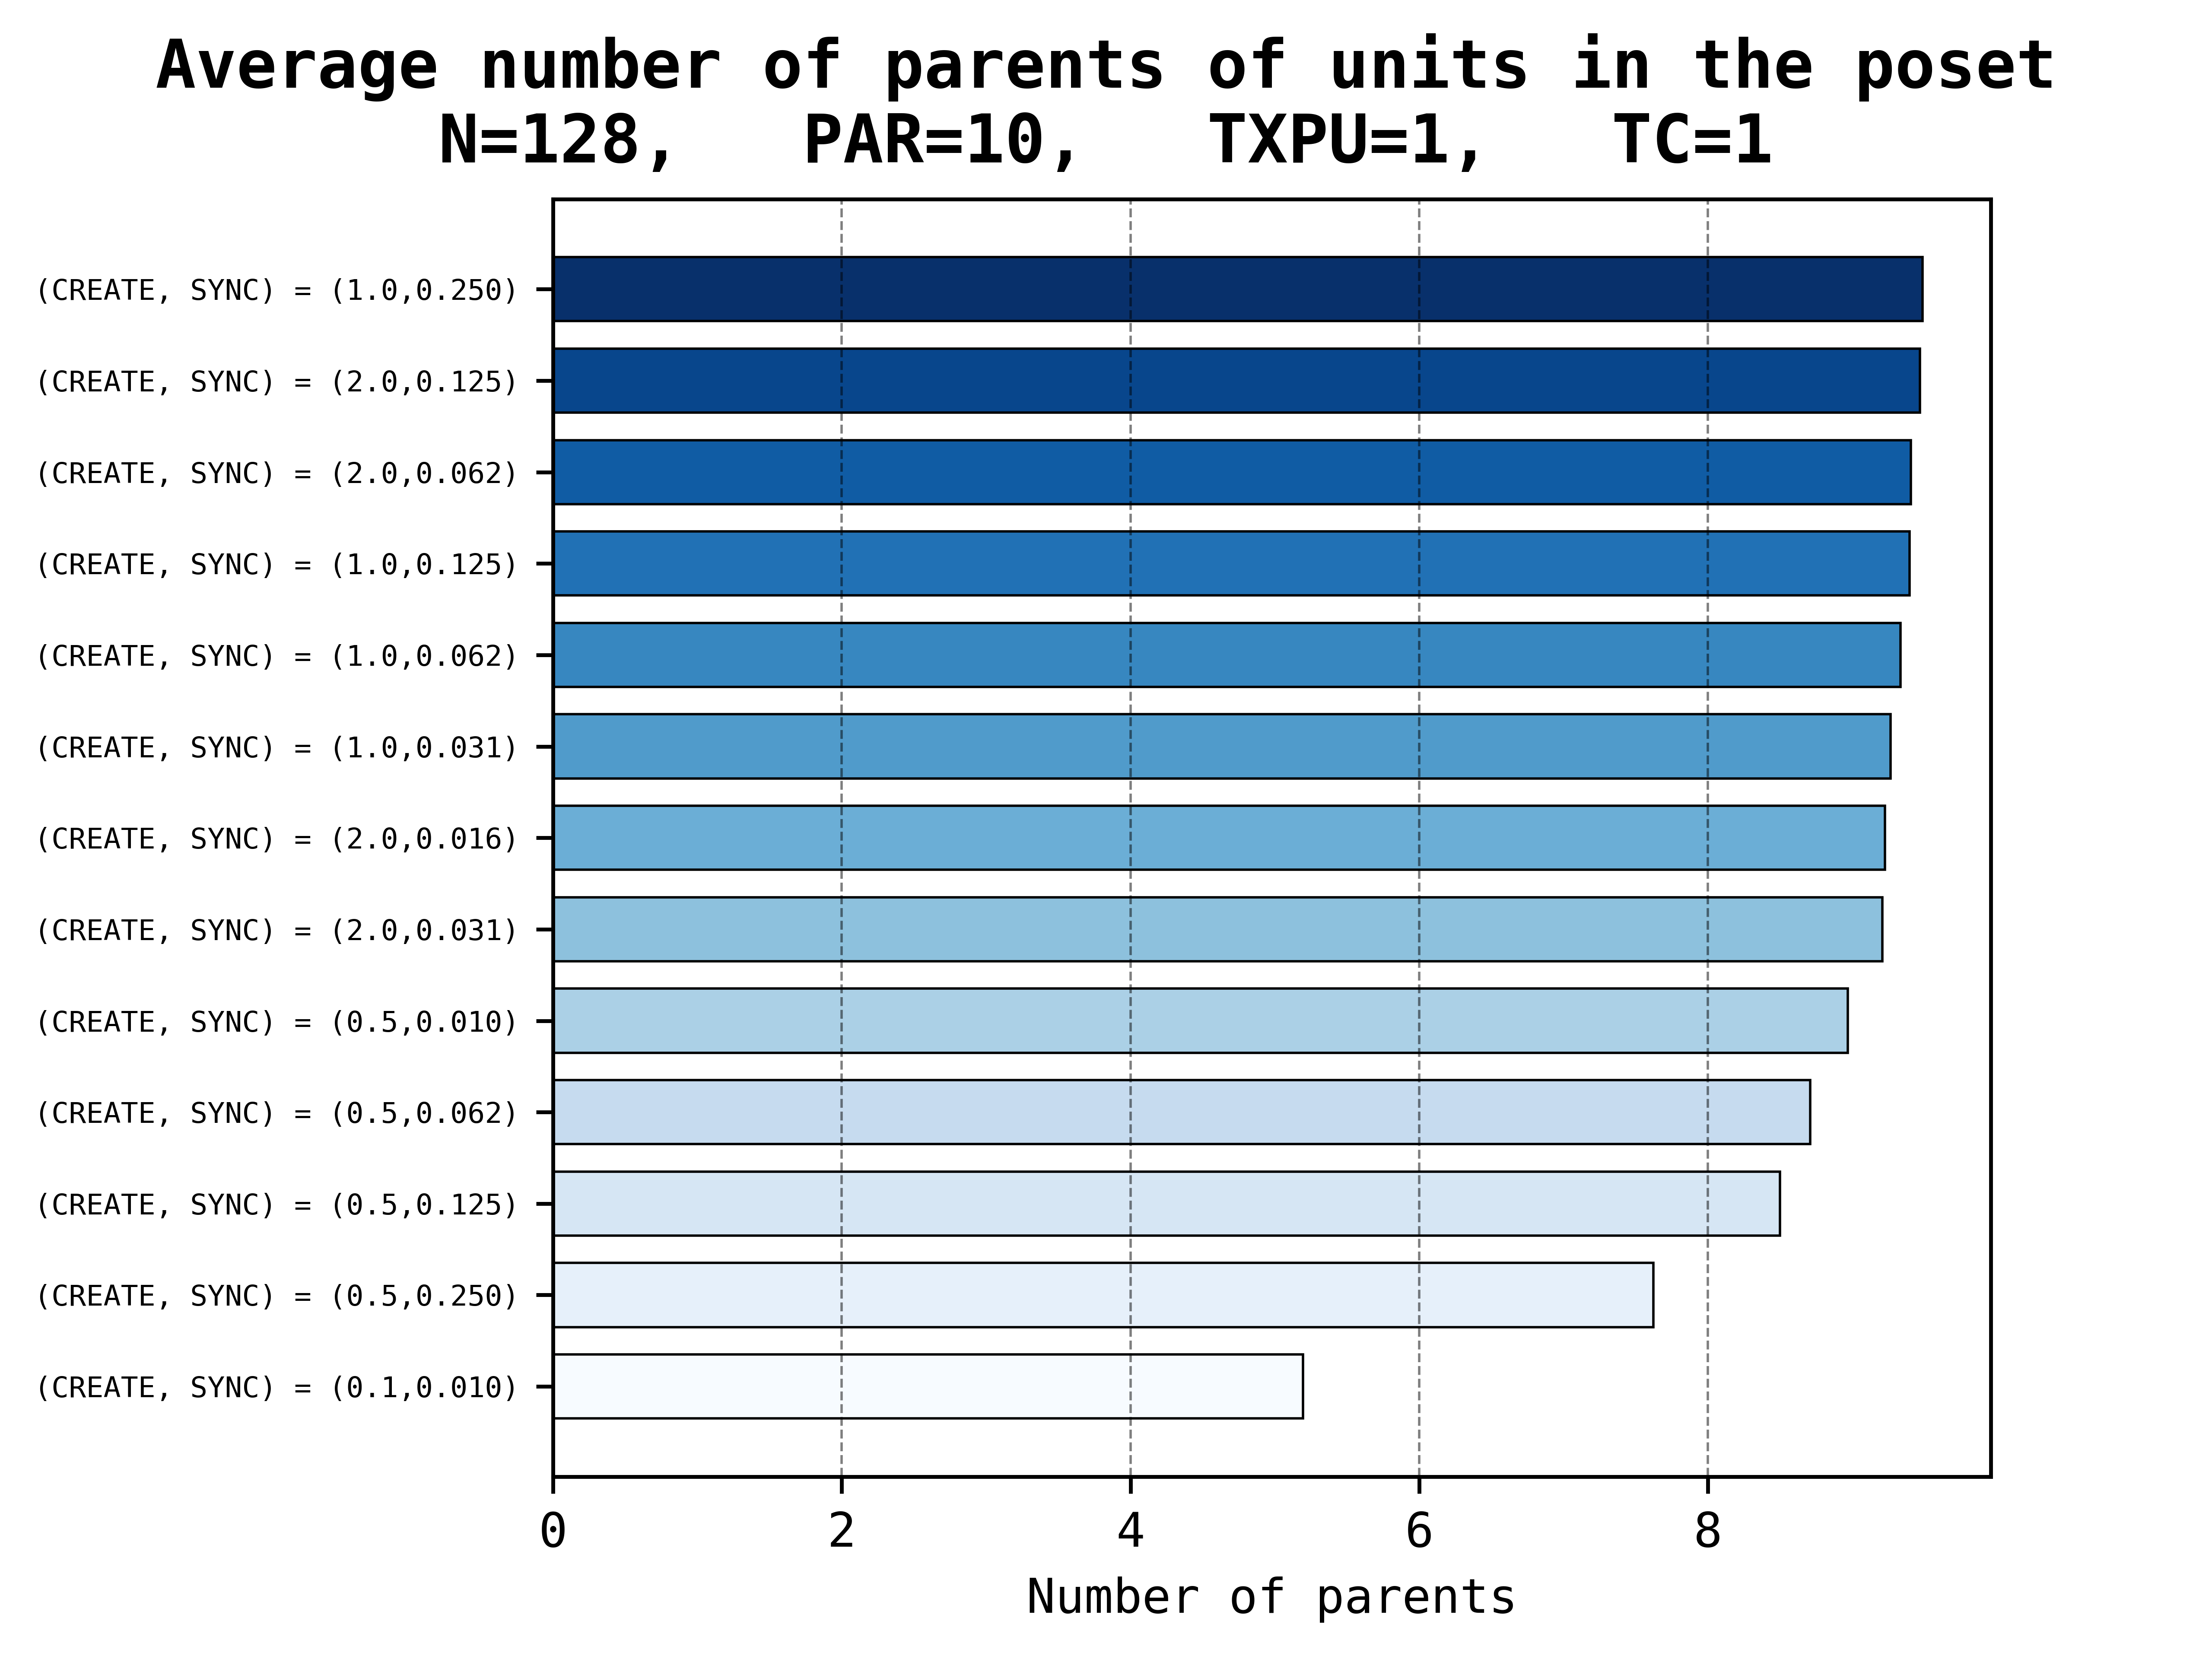
\includegraphics[width=0.8\textwidth]{bar_plots/final_exp1/n_parents.png}
				\caption{The average number of parents per unit.}
				\label{fig:delaysParents}
			\end{figure}
			\begin{figure}[h]
				\centering
				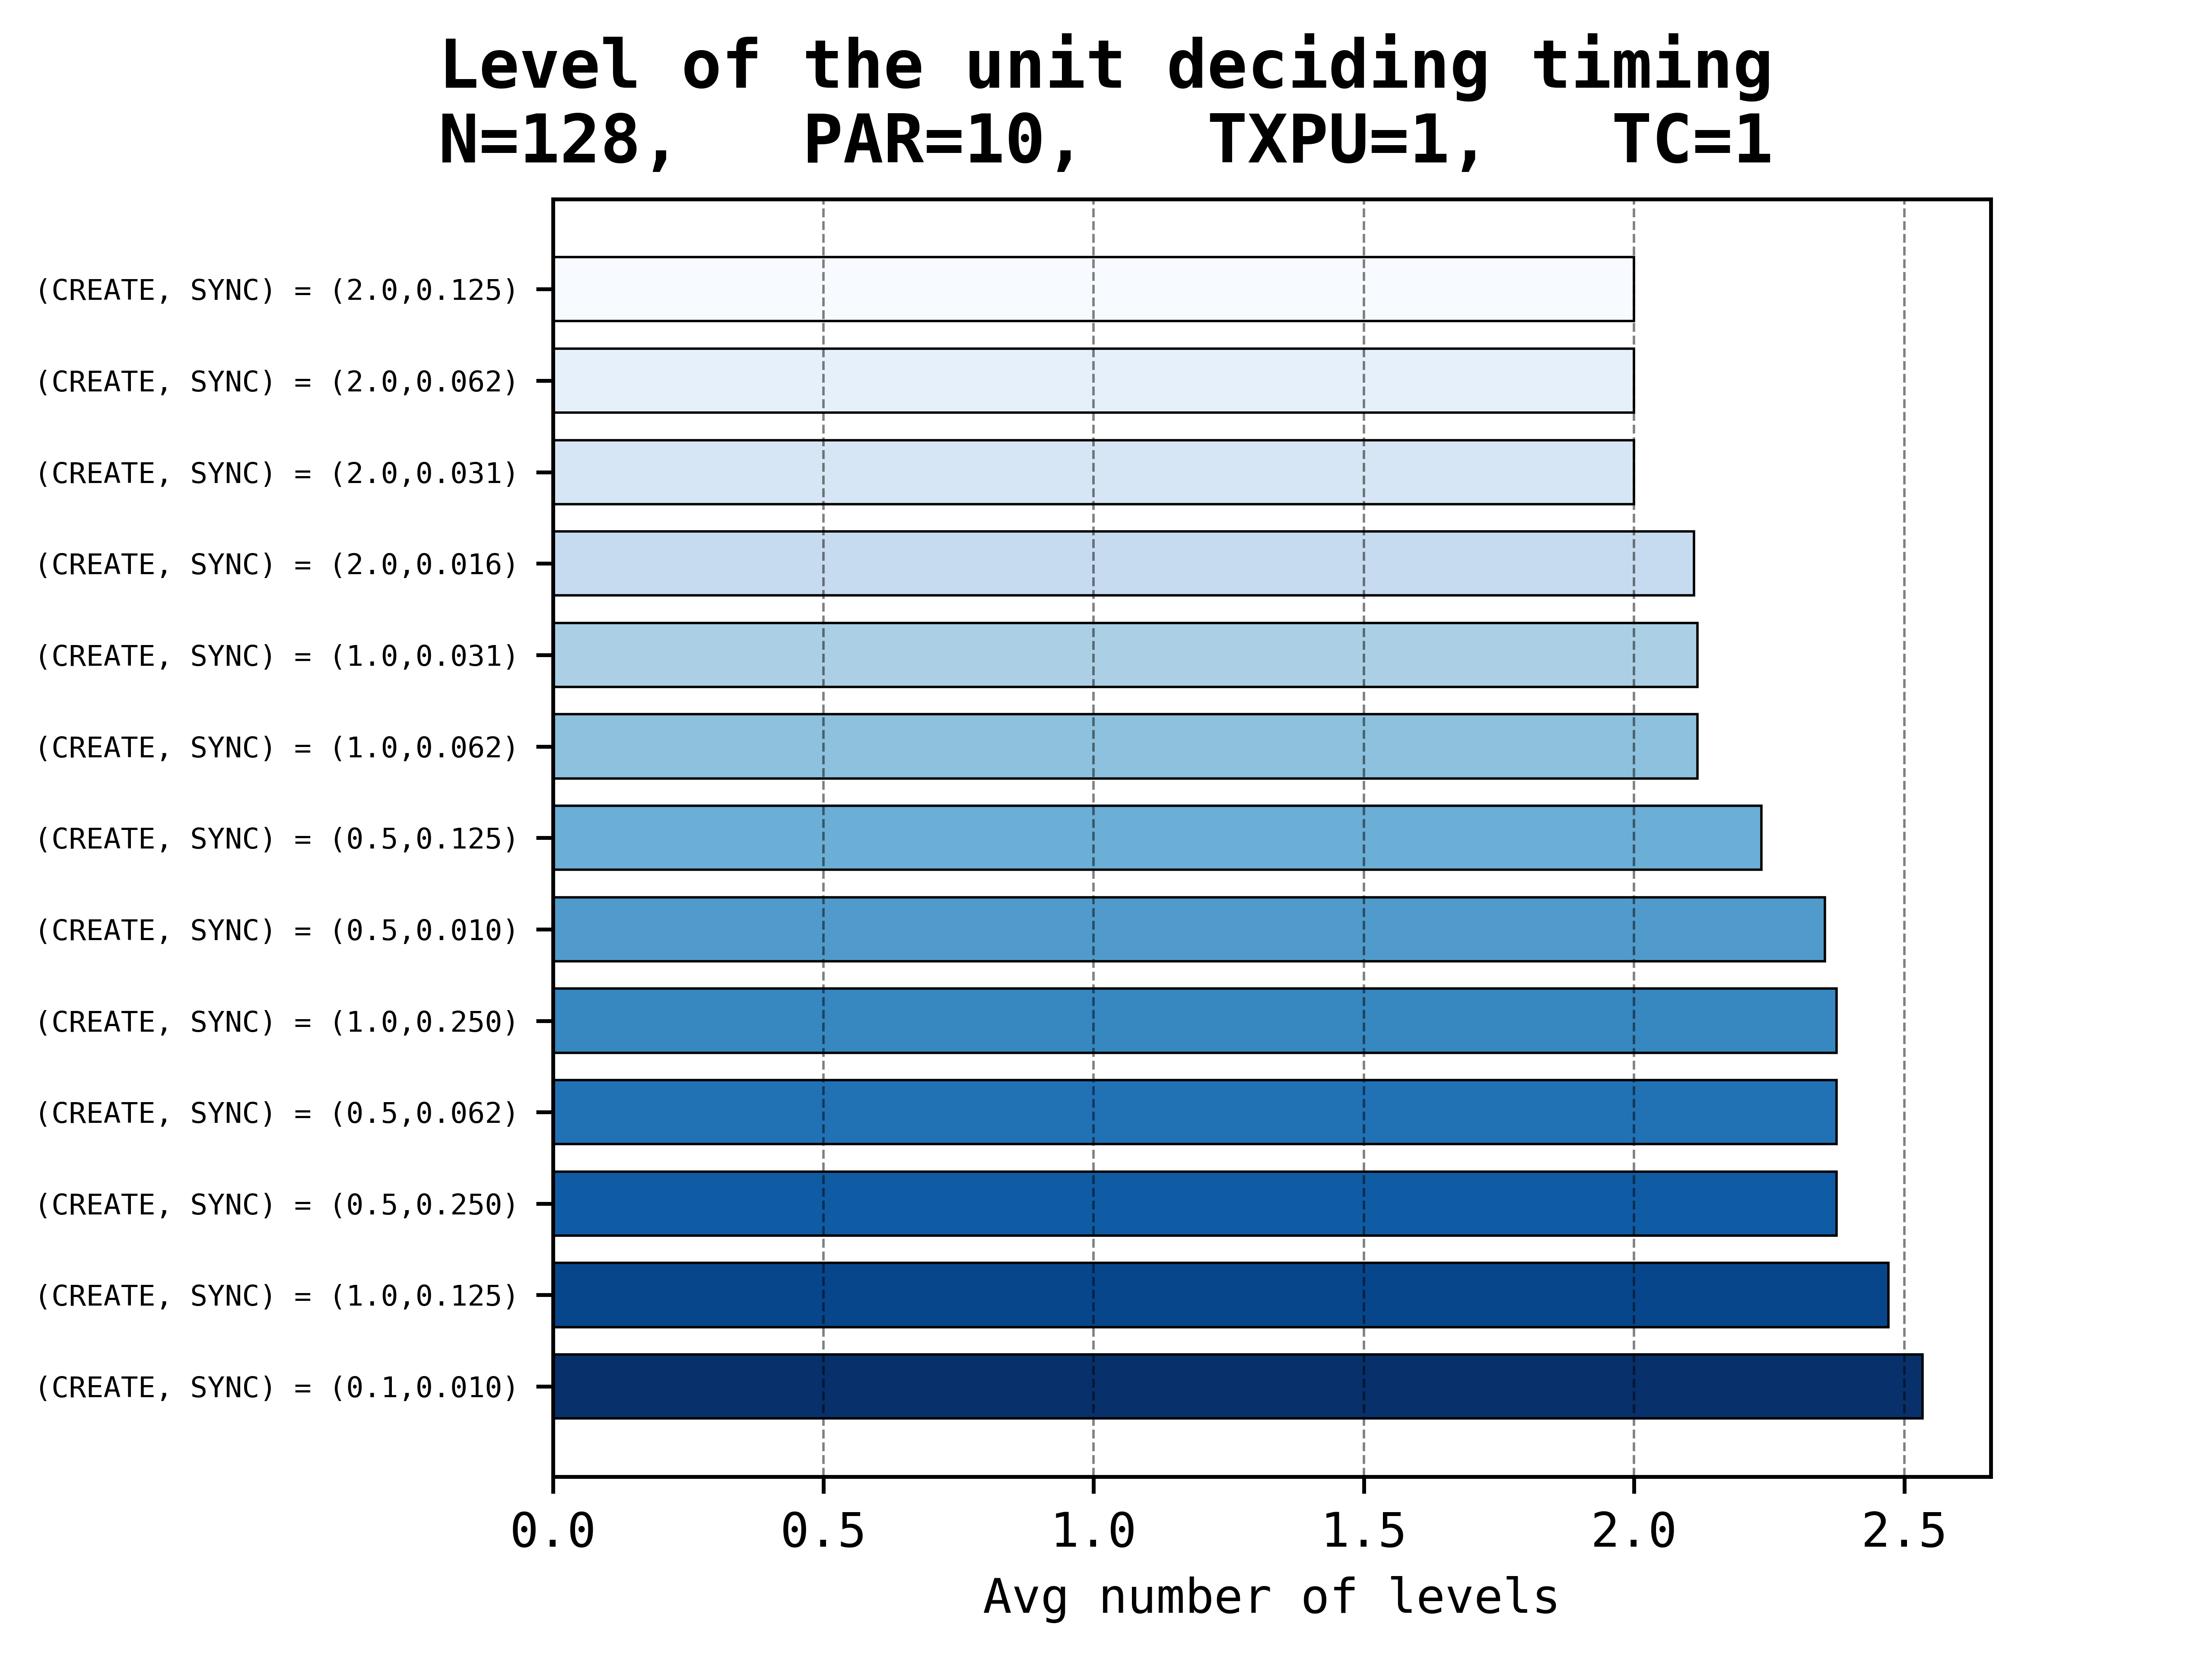
\includegraphics[width=0.8\textwidth]{bar_plots/final_exp1/decision_height.png}
				\caption{How many levels above the considered unit was the timing decision taken, on average.}
				\label{fig:delaysDecisionUnit}
			\end{figure}
			\begin{figure}[h]
				\centering
				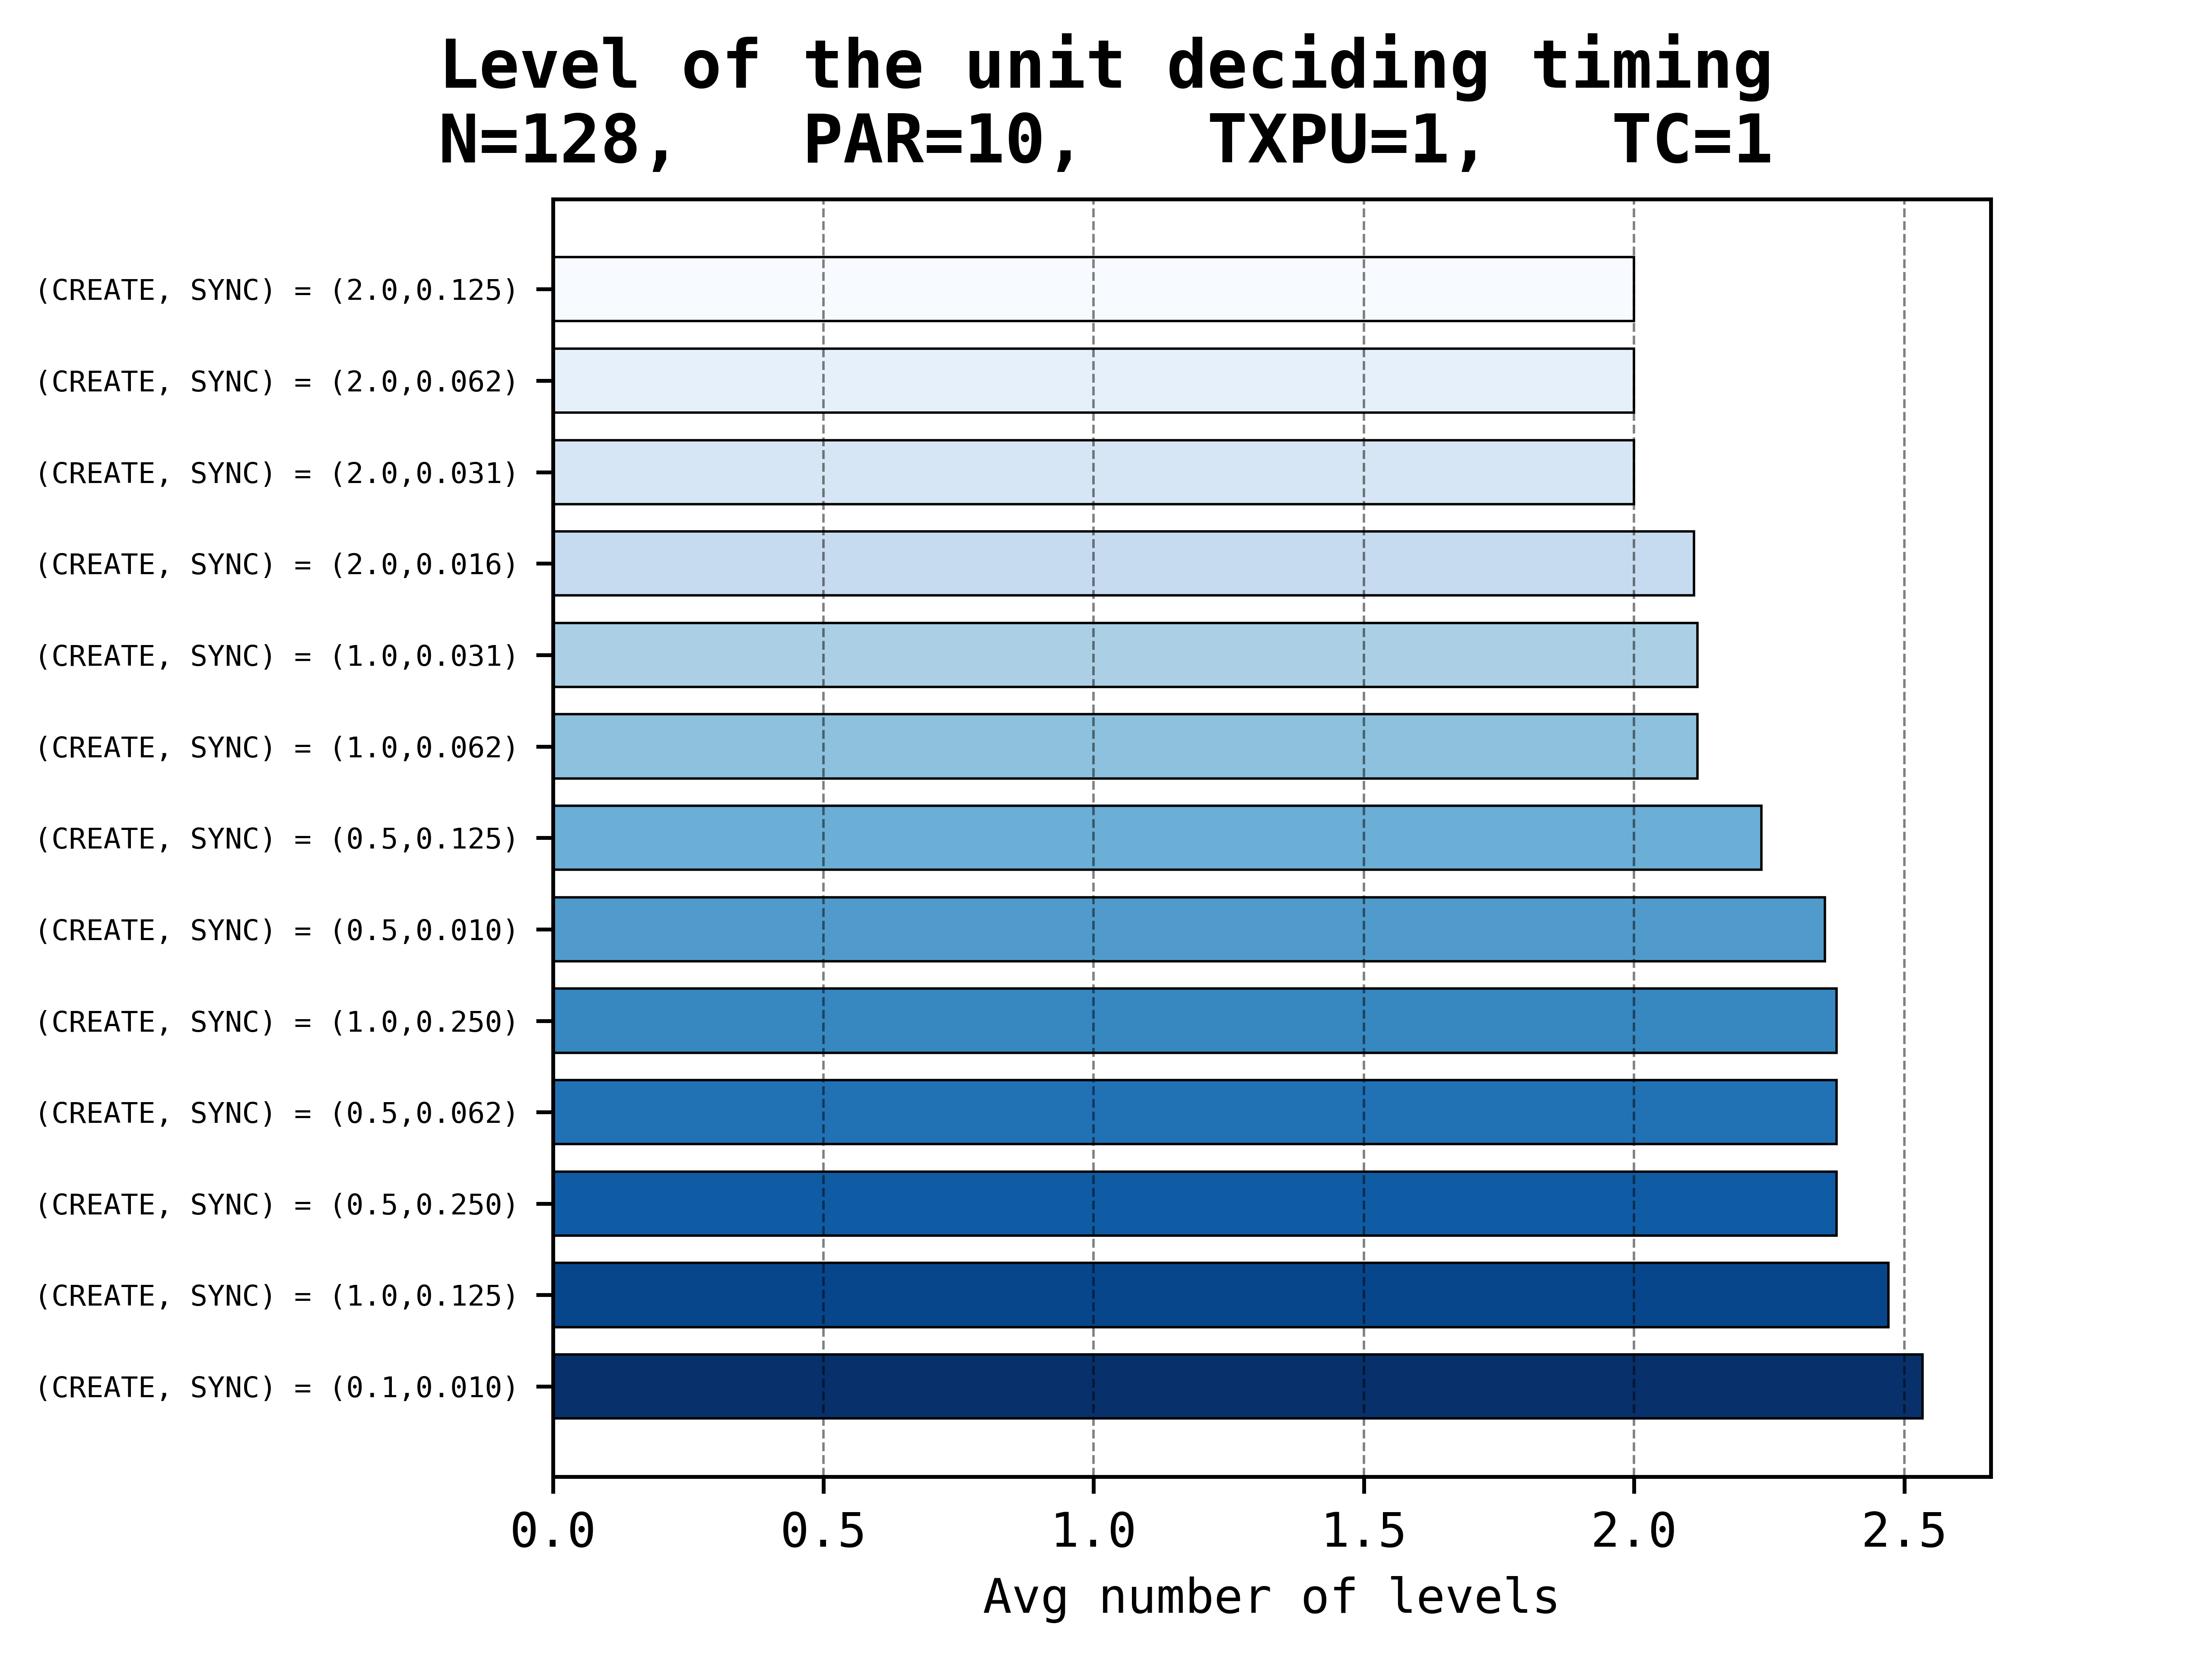
\includegraphics[width=0.8\textwidth]{bar_plots/final_exp1/decision_height.png}
				\caption{How many levels above the considered unit was the maximal unit in the poset when the timing decision was made, on average. Compare with Figure \ref{fig:delaysDecisionUnit}.}
				\label{fig:delaysDecisionPoset}
			\end{figure}
			\begin{figure}[h]
				\centering
				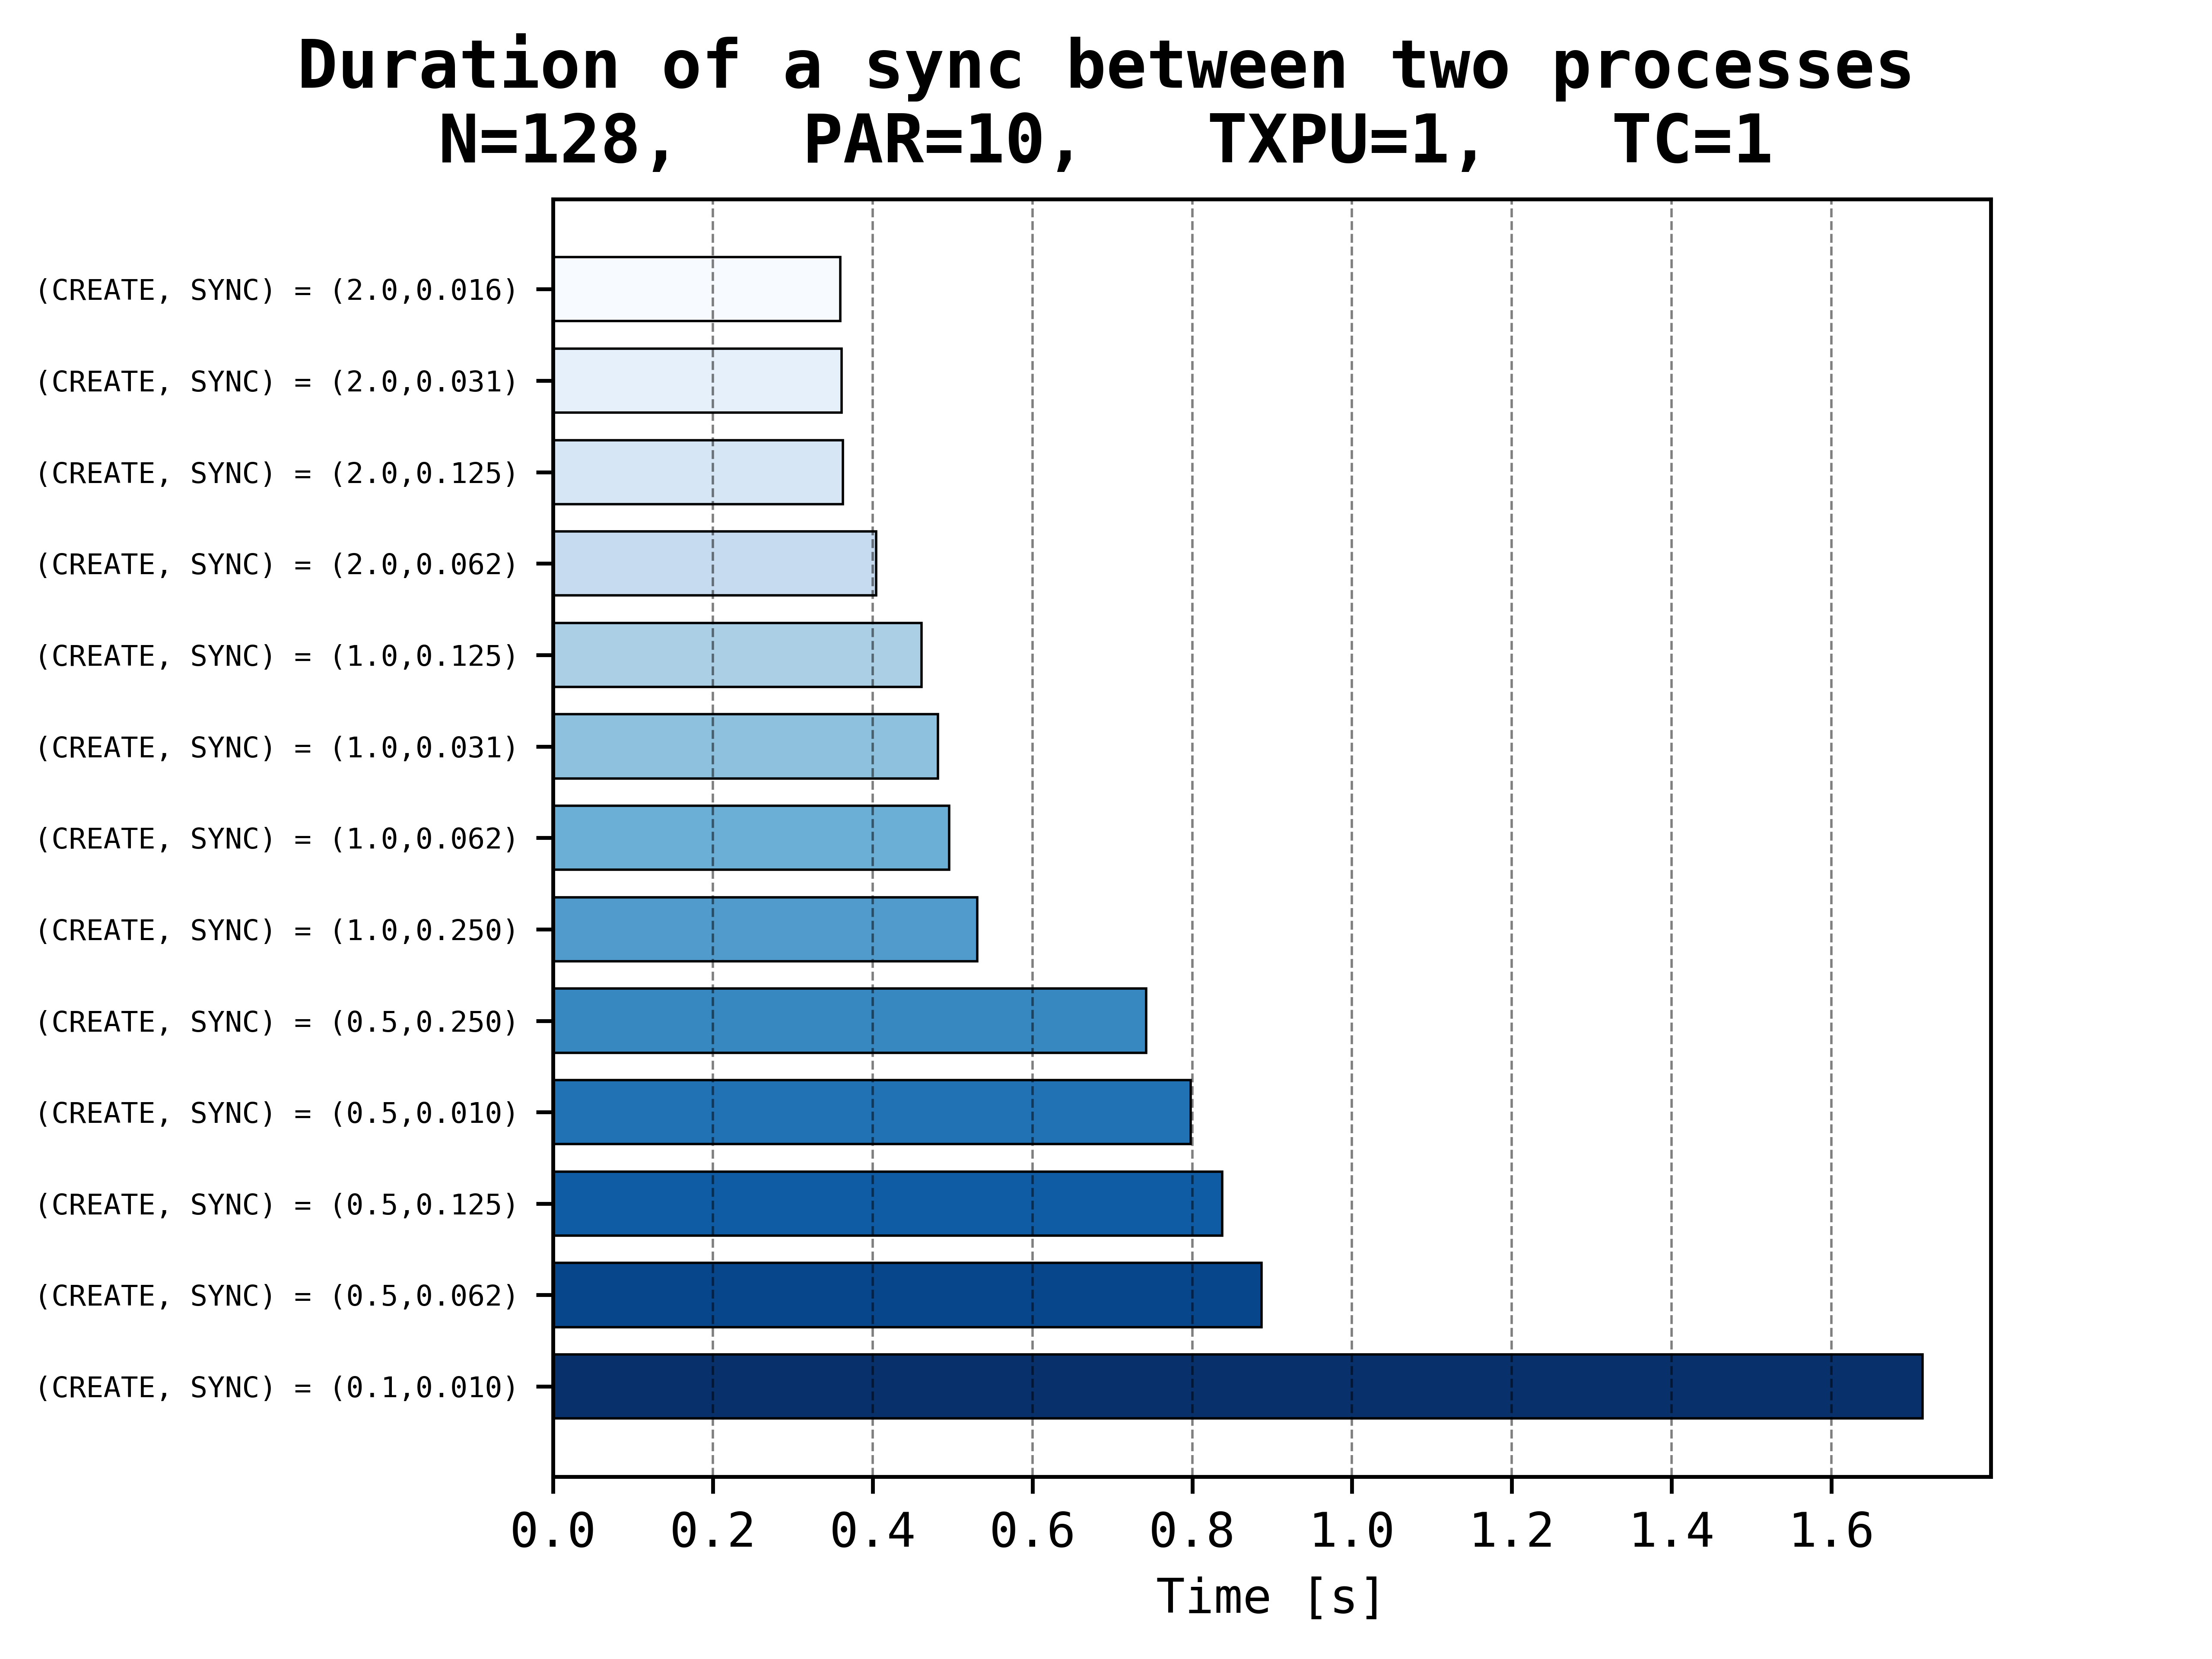
\includegraphics[width=0.8\textwidth]{bar_plots/final_exp1/time_per_sync.png}
				\caption{The average time a single sync operation took.}
				\label{fig:delaysTimePerSync}
			\end{figure}
			\begin{figure}[h]
				\centering
				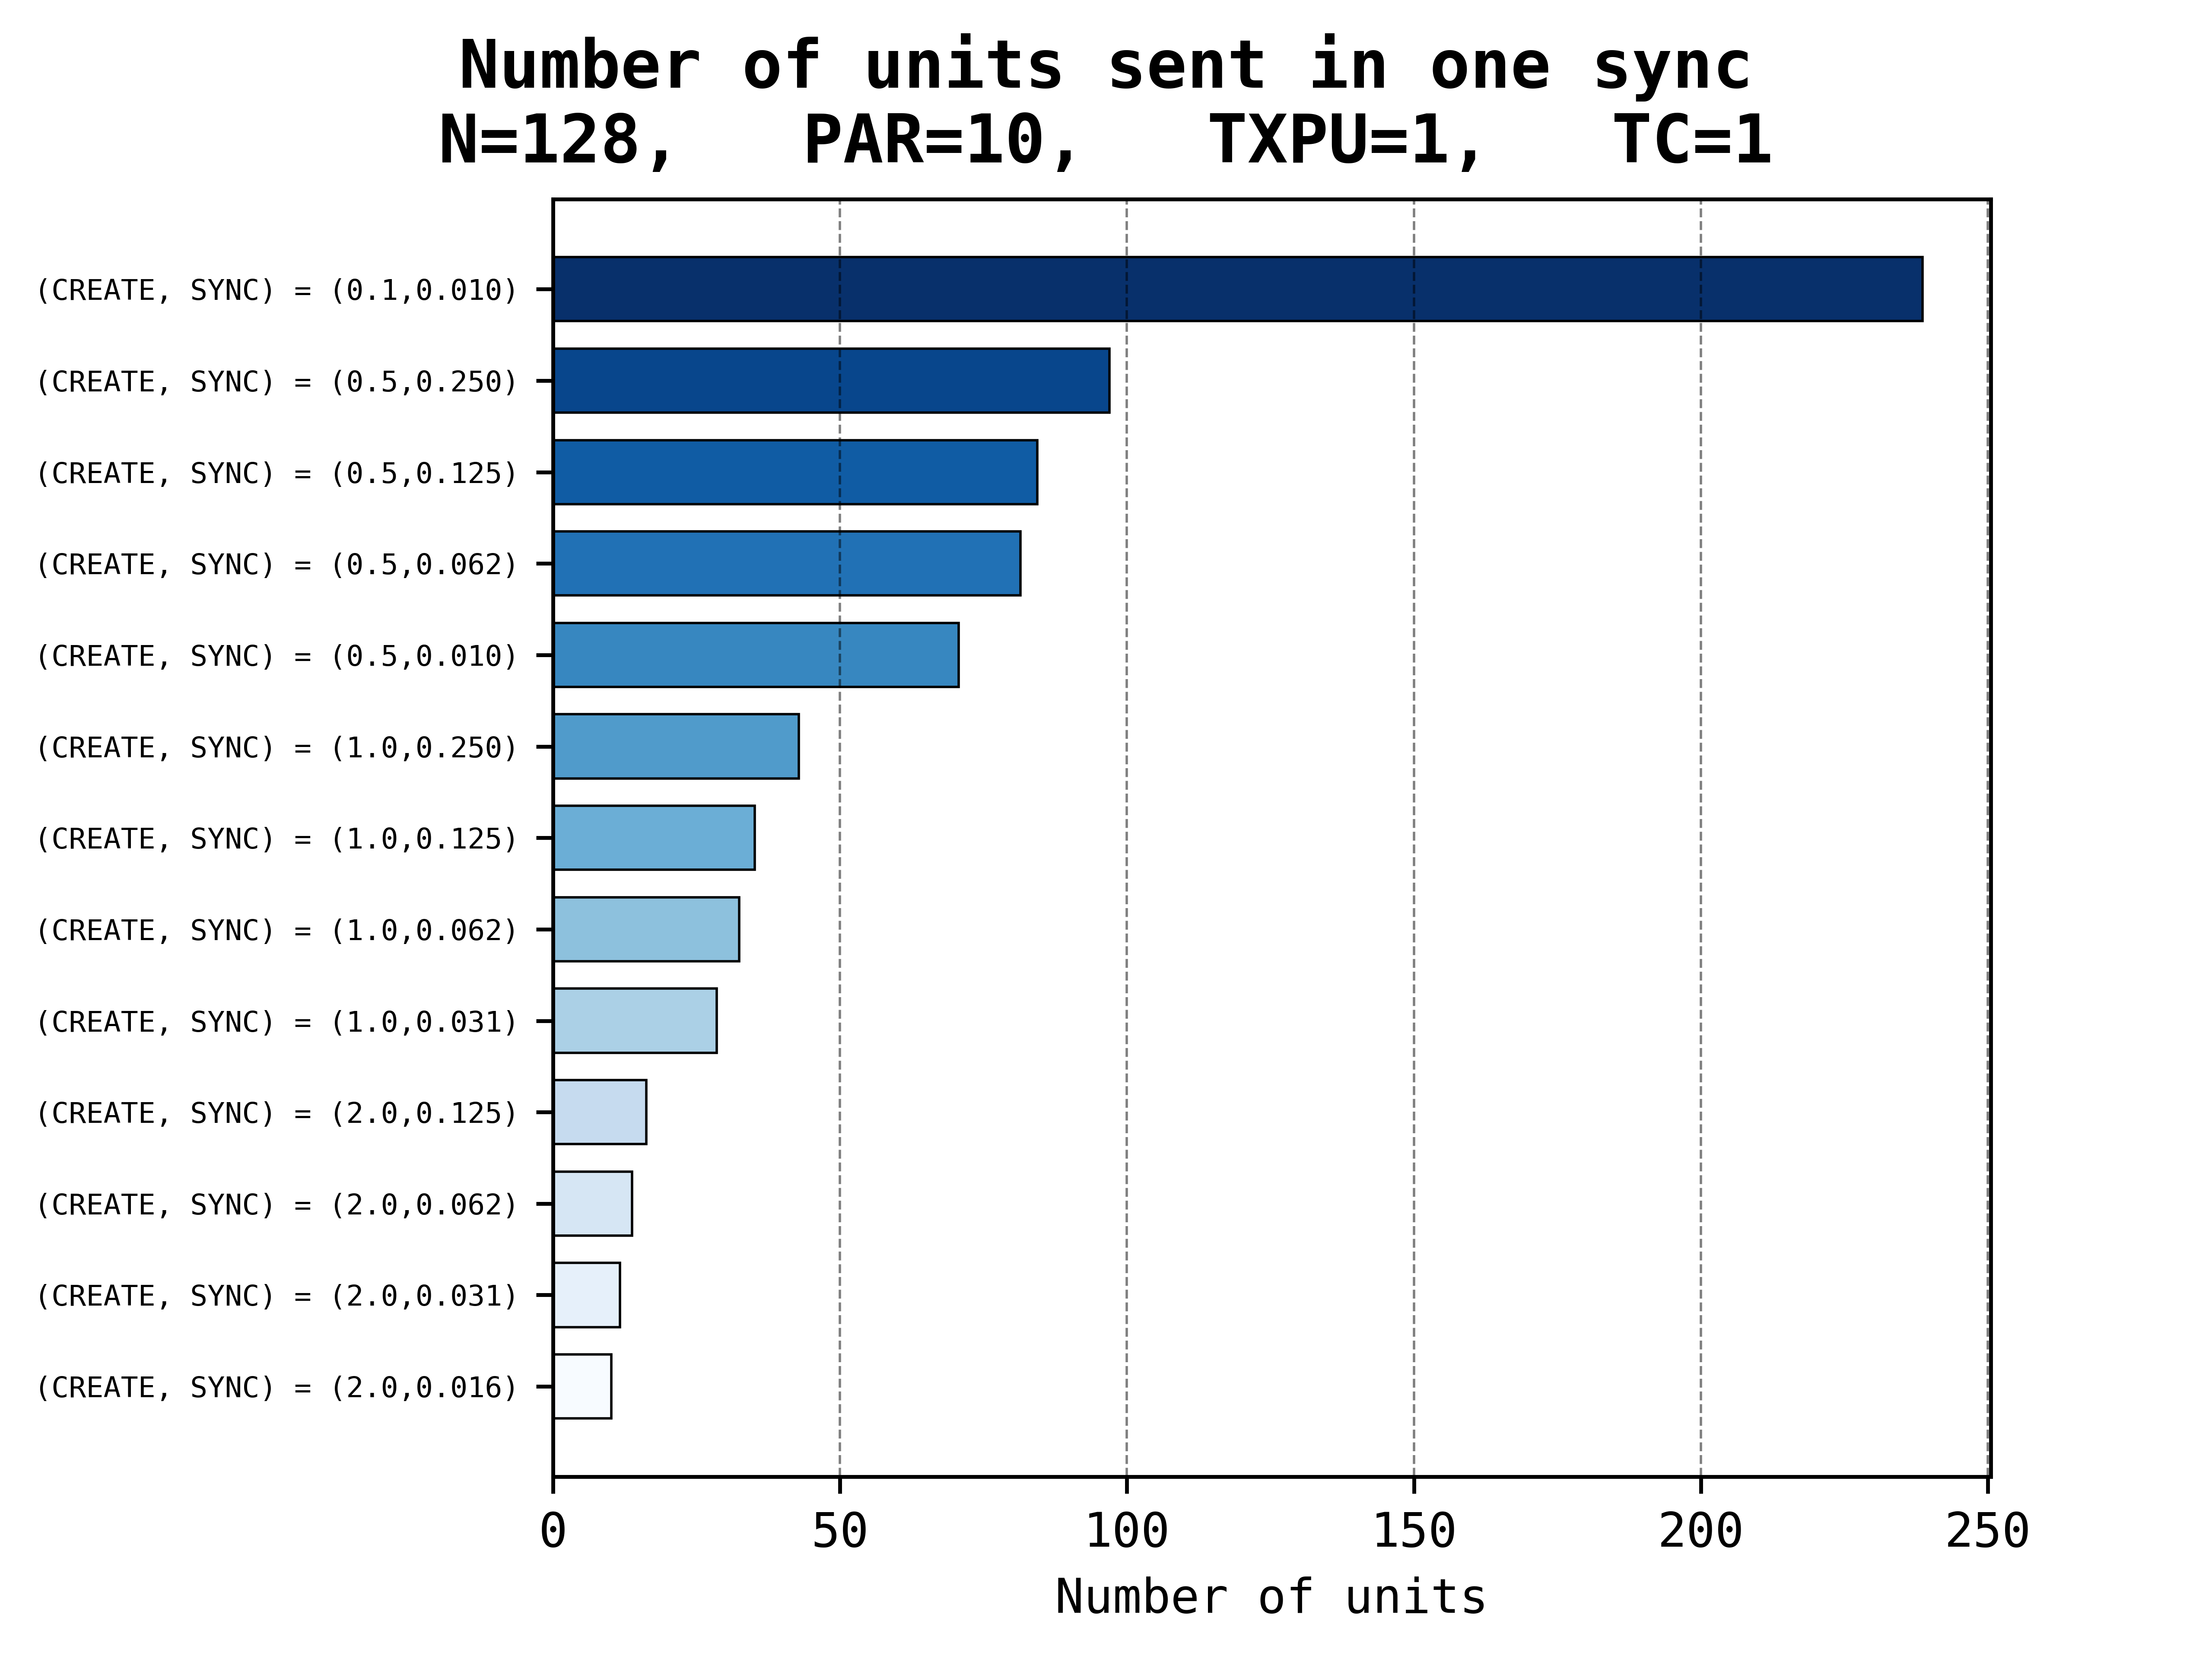
\includegraphics[width=0.8\textwidth]{bar_plots/final_exp1/units_sent_sync.png}
				\caption{The average number of units sent per sync.}
				\label{fig:delaysUnitsPerSync}
			\end{figure}
			\begin{figure}[h]
				\centering
				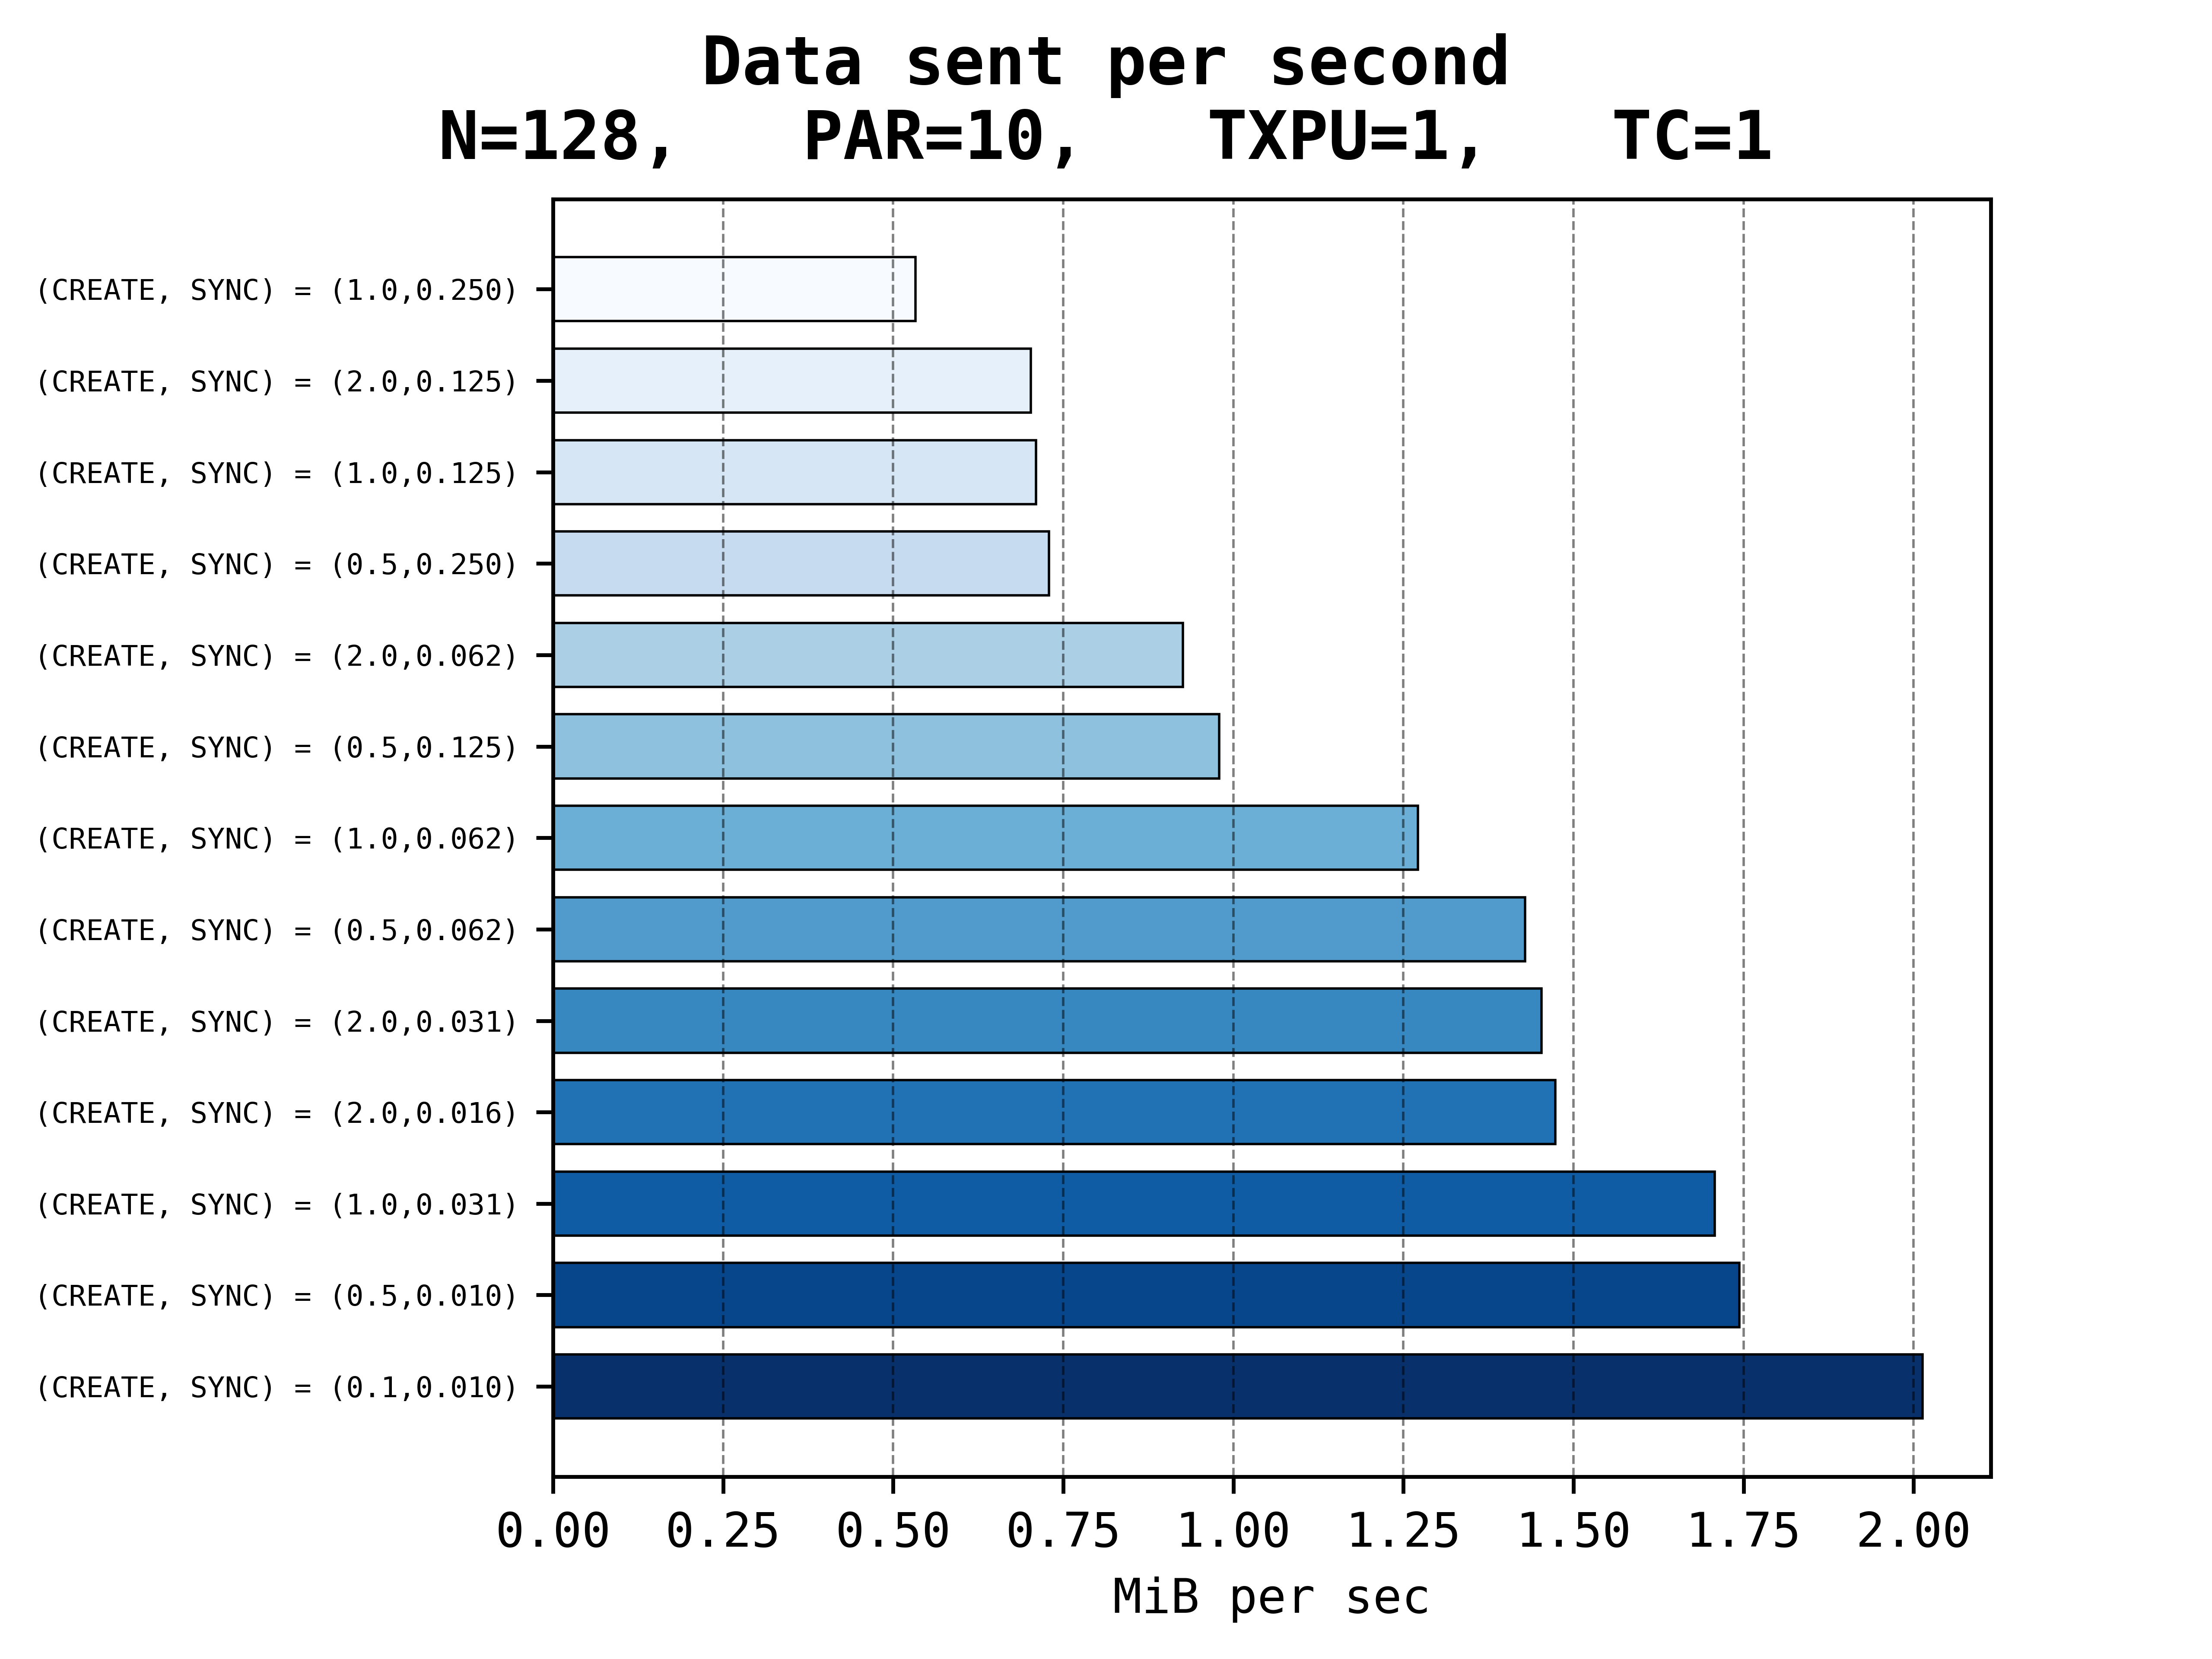
\includegraphics[width=0.8\textwidth]{bar_plots/final_exp1/bytes_sent_per_sec.png}
				\caption{The average amount of data sent per second.}
				\label{fig:delaysBps}
			\end{figure}
		\FloatBarrier
		\subsection{Transactions}
		\FloatBarrier
			The second series of experiments was designed mostly to check the relation between transactions per unit, validation latency, and committee size.
			In all tests there were maximally $10$ parents, $10$ simultaneous incoming/outgoing connections, and the sync delay was $.125$.
			Other values can be seen in the graphs.
			\begin{figure}[h]
				\centering
				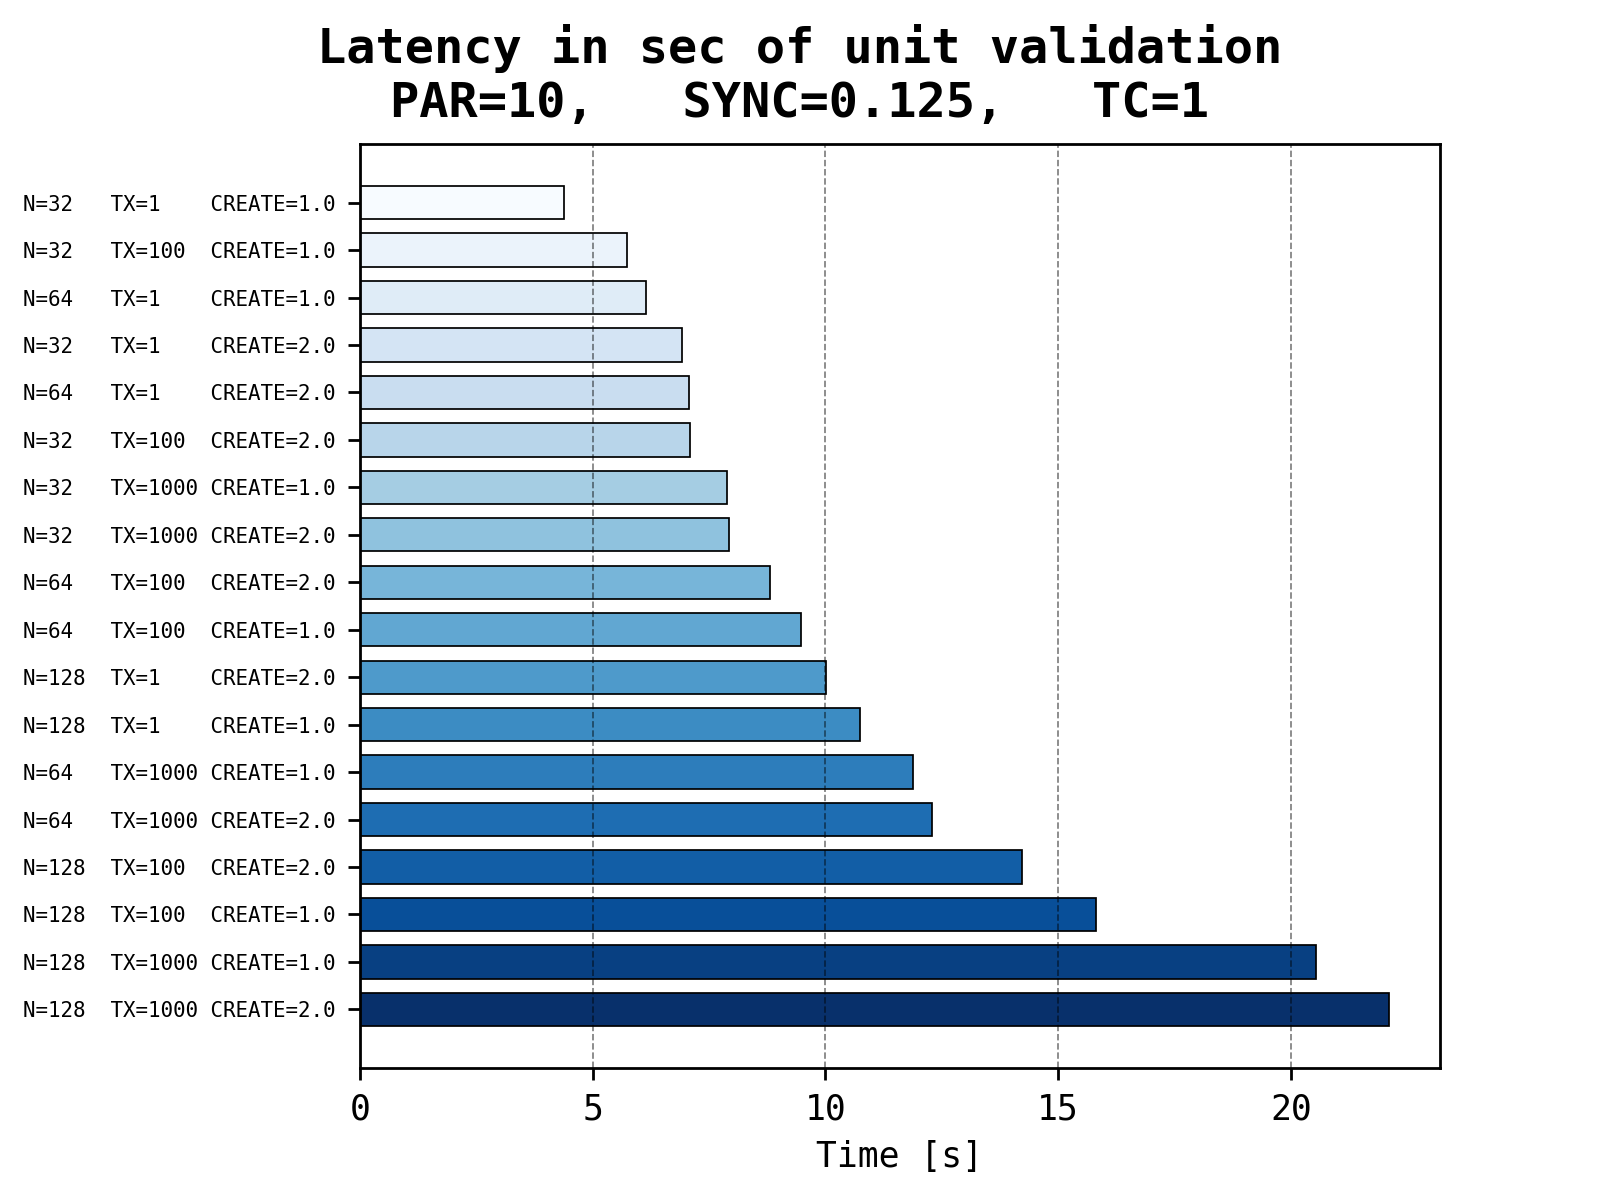
\includegraphics[width=0.8\textwidth]{bar_plots/final_exp2/create_ord_del.png}
				\caption{The latency of unit validation in the second series of experiments.}
				\label{fig:transactionsLatency}
			\end{figure}
			\begin{figure}[h]
				\centering
				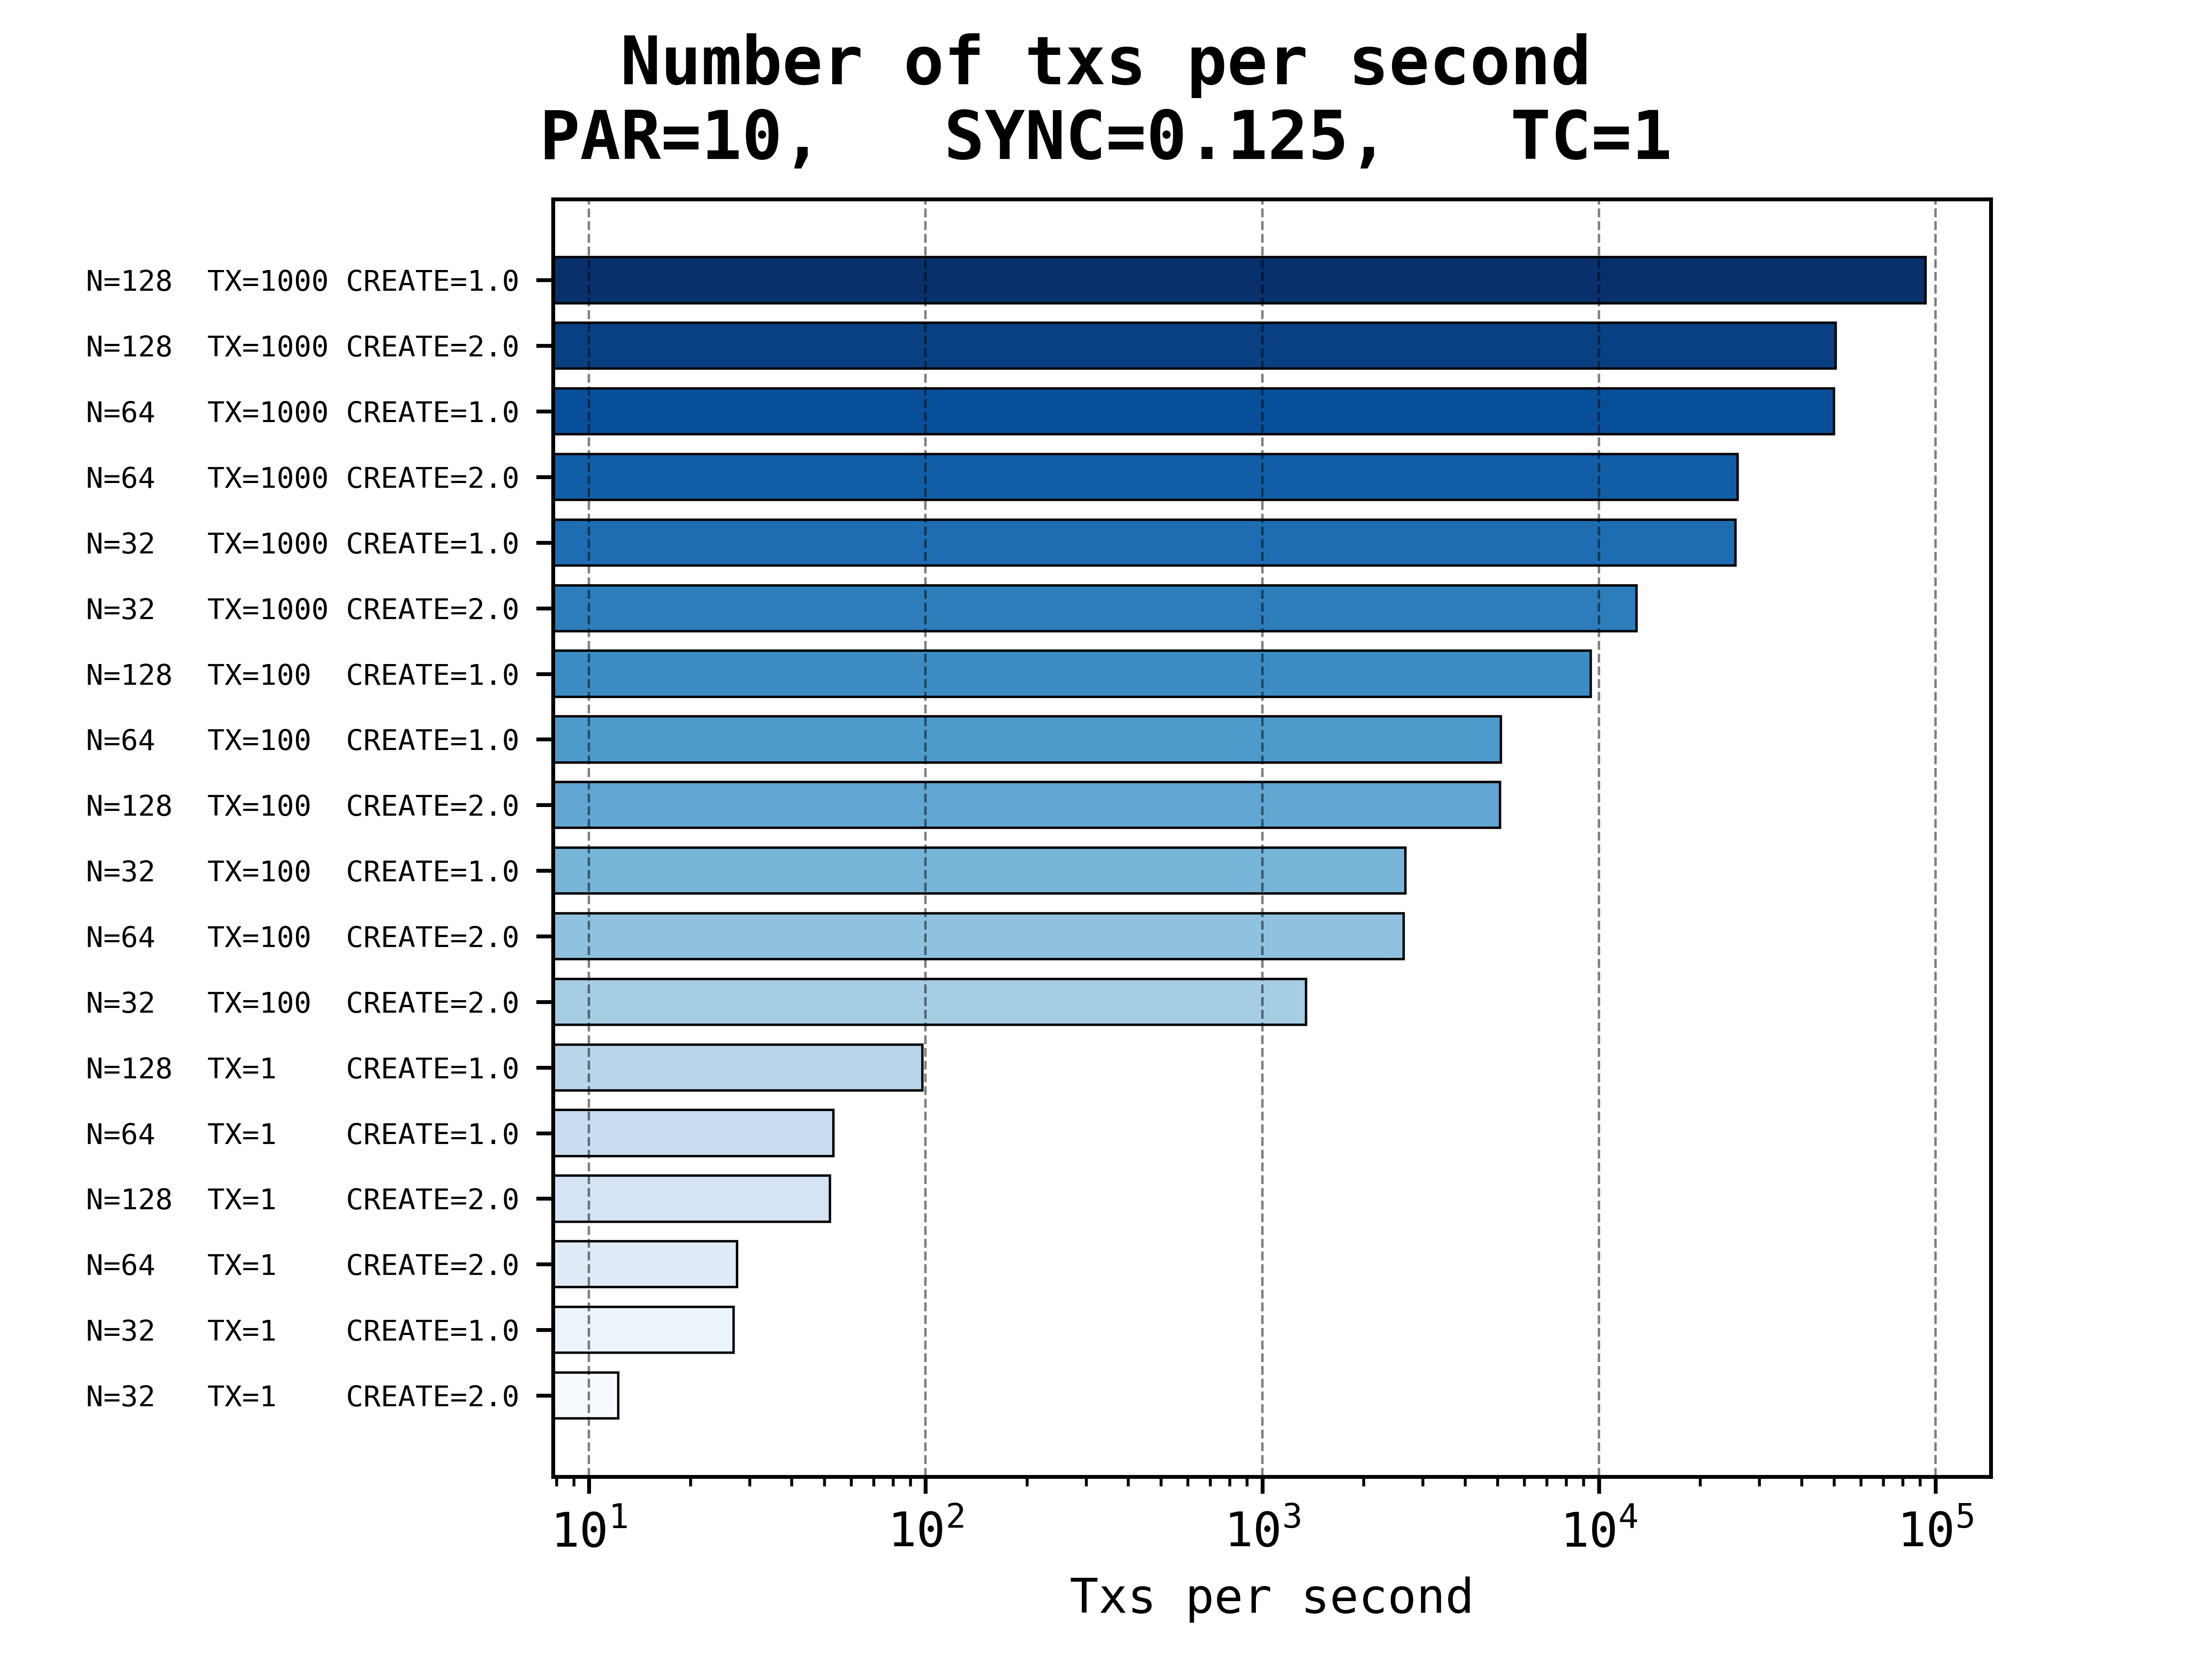
\includegraphics[width=0.8\textwidth]{bar_plots/final_exp2/txps.png}
				\caption{The number of transaction entering the system per second.}
				\label{fig:transactionsTxps}
			\end{figure}
			\begin{figure}[h]
				\centering
				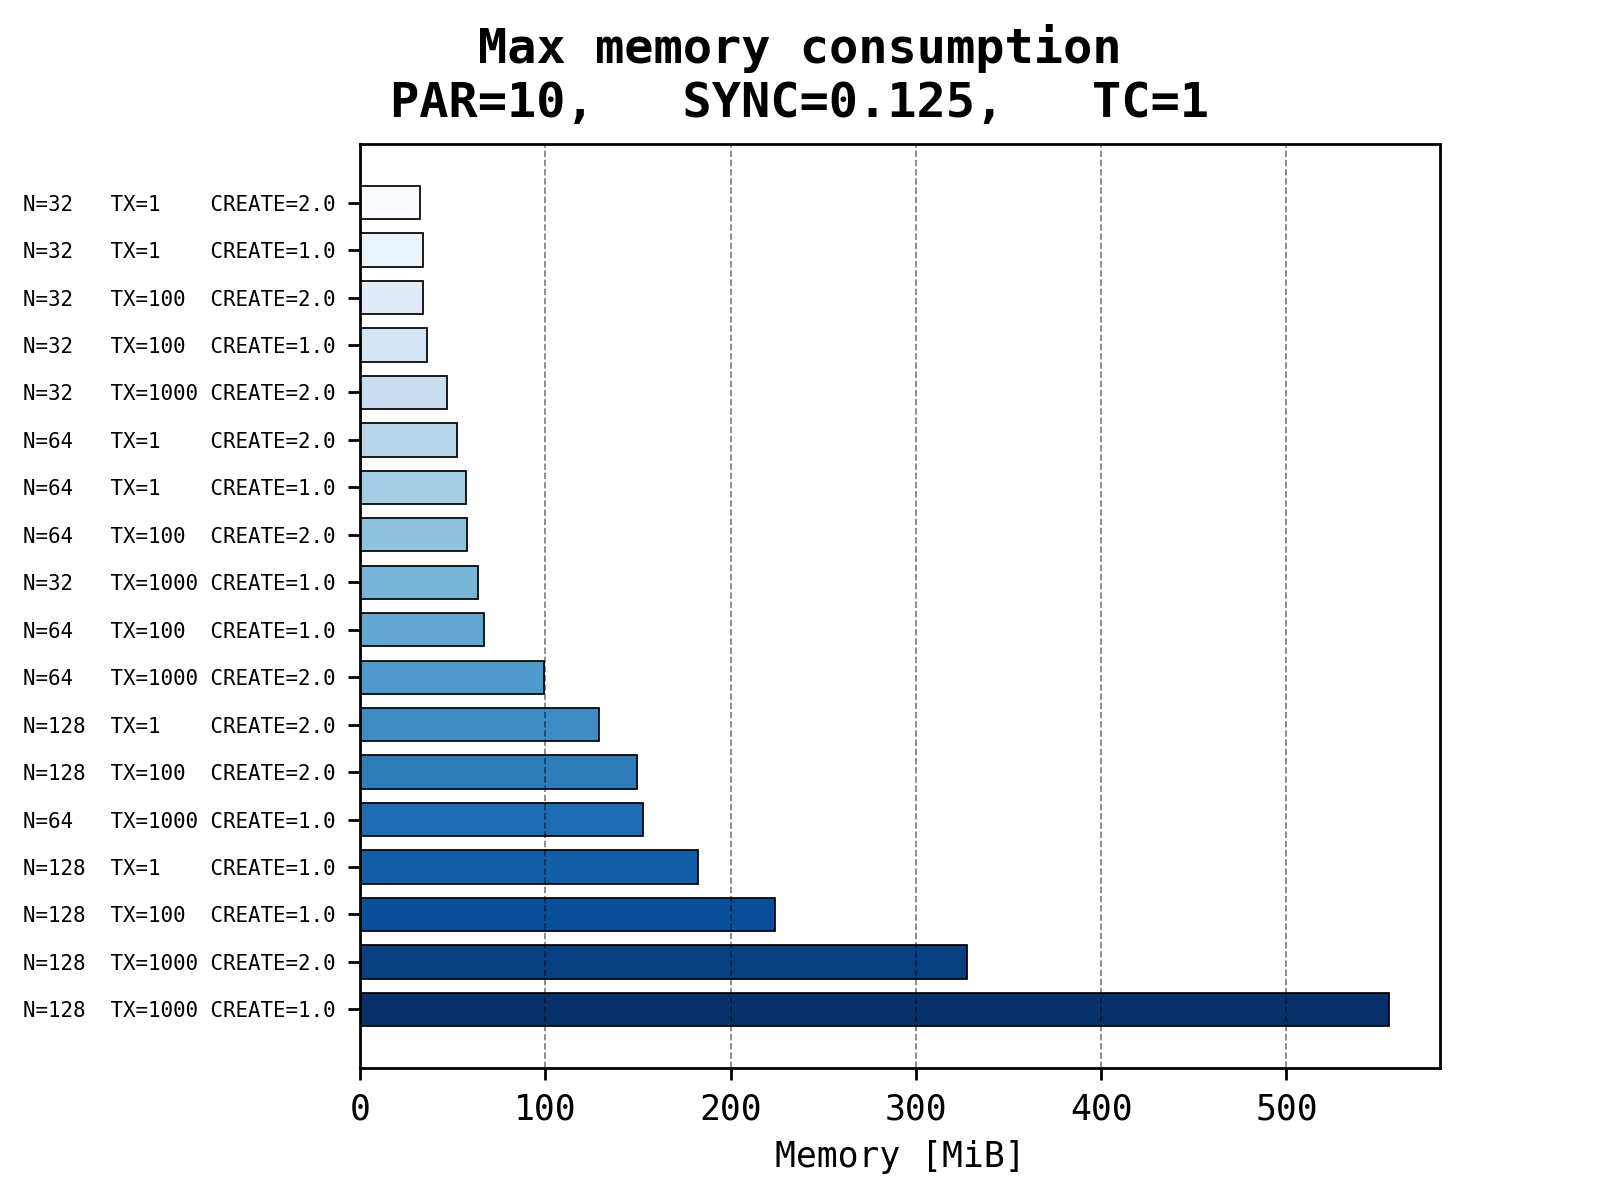
\includegraphics[width=0.8\textwidth]{bar_plots/final_exp2/memory_MiB.png}
				\caption{The amount of RAM used by a process.}
				\label{fig:transactionsRAM}
			\end{figure}
			\begin{figure}[h]
				\centering
				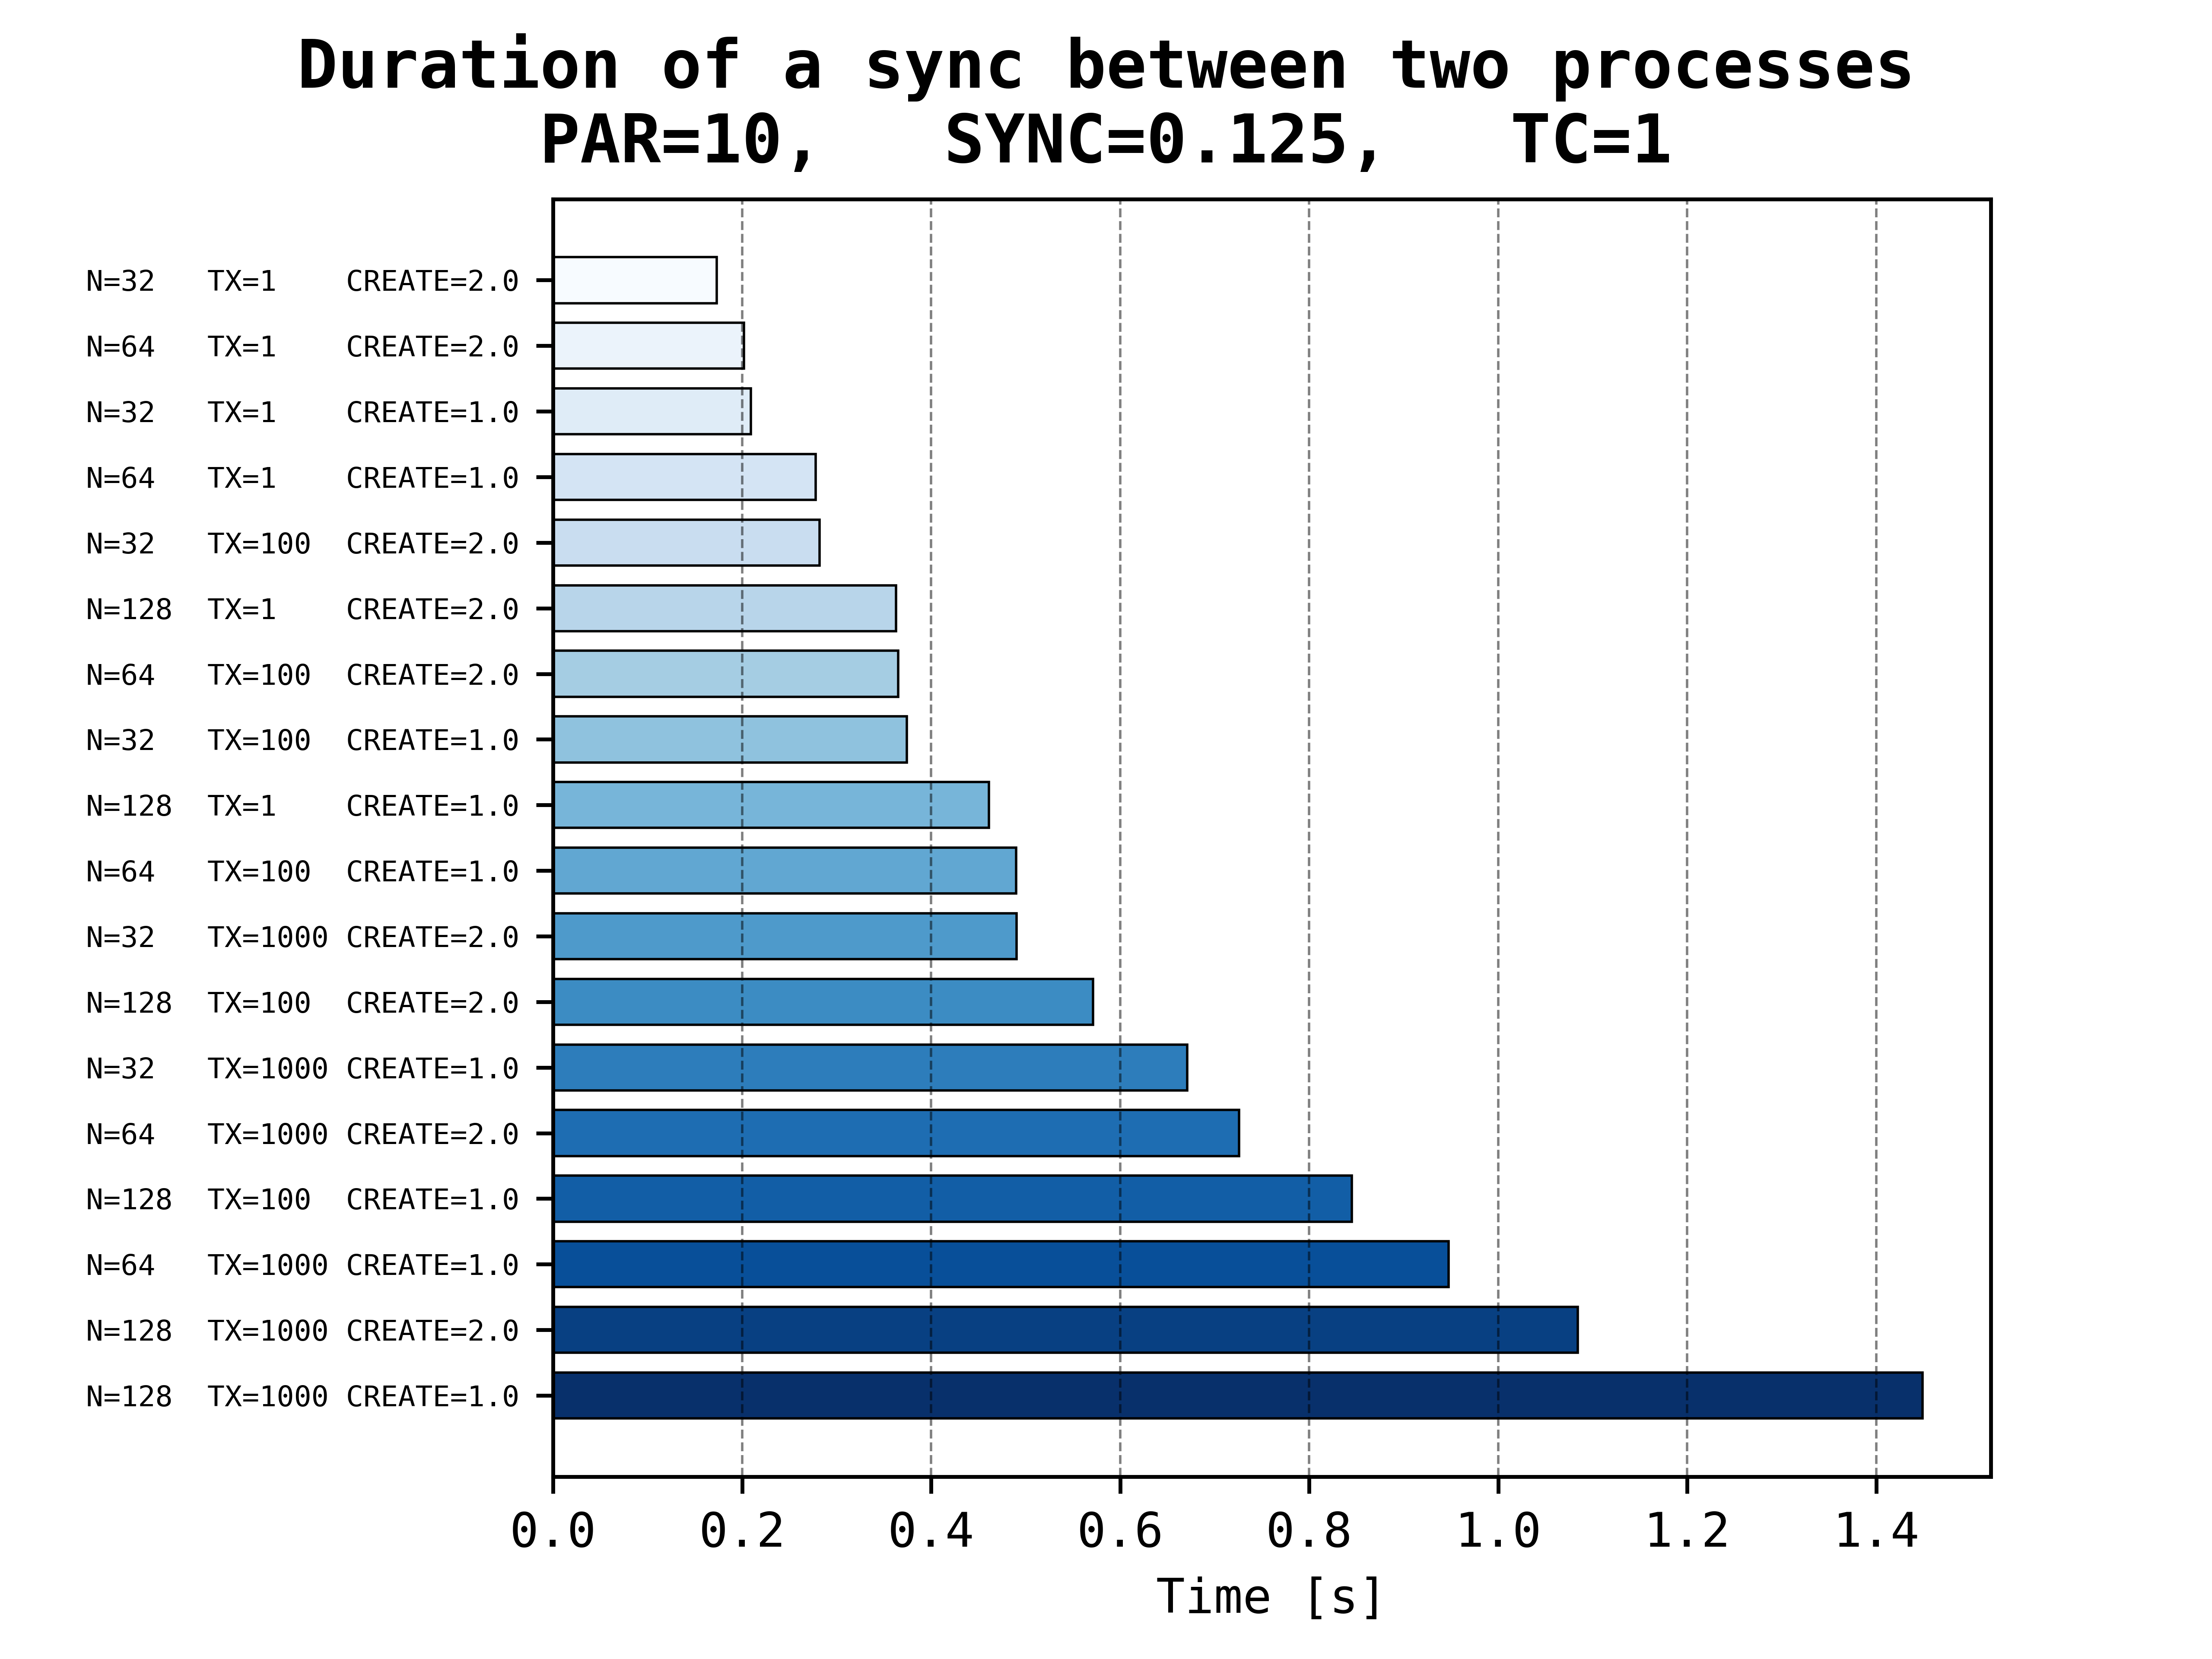
\includegraphics[width=0.8\textwidth]{bar_plots/final_exp2/time_per_sync.png}
				\caption{The average time a single sync operation took.}
				\label{fig:transactionsTimePerSync}
			\end{figure}
			\begin{figure}[h]
				\centering
				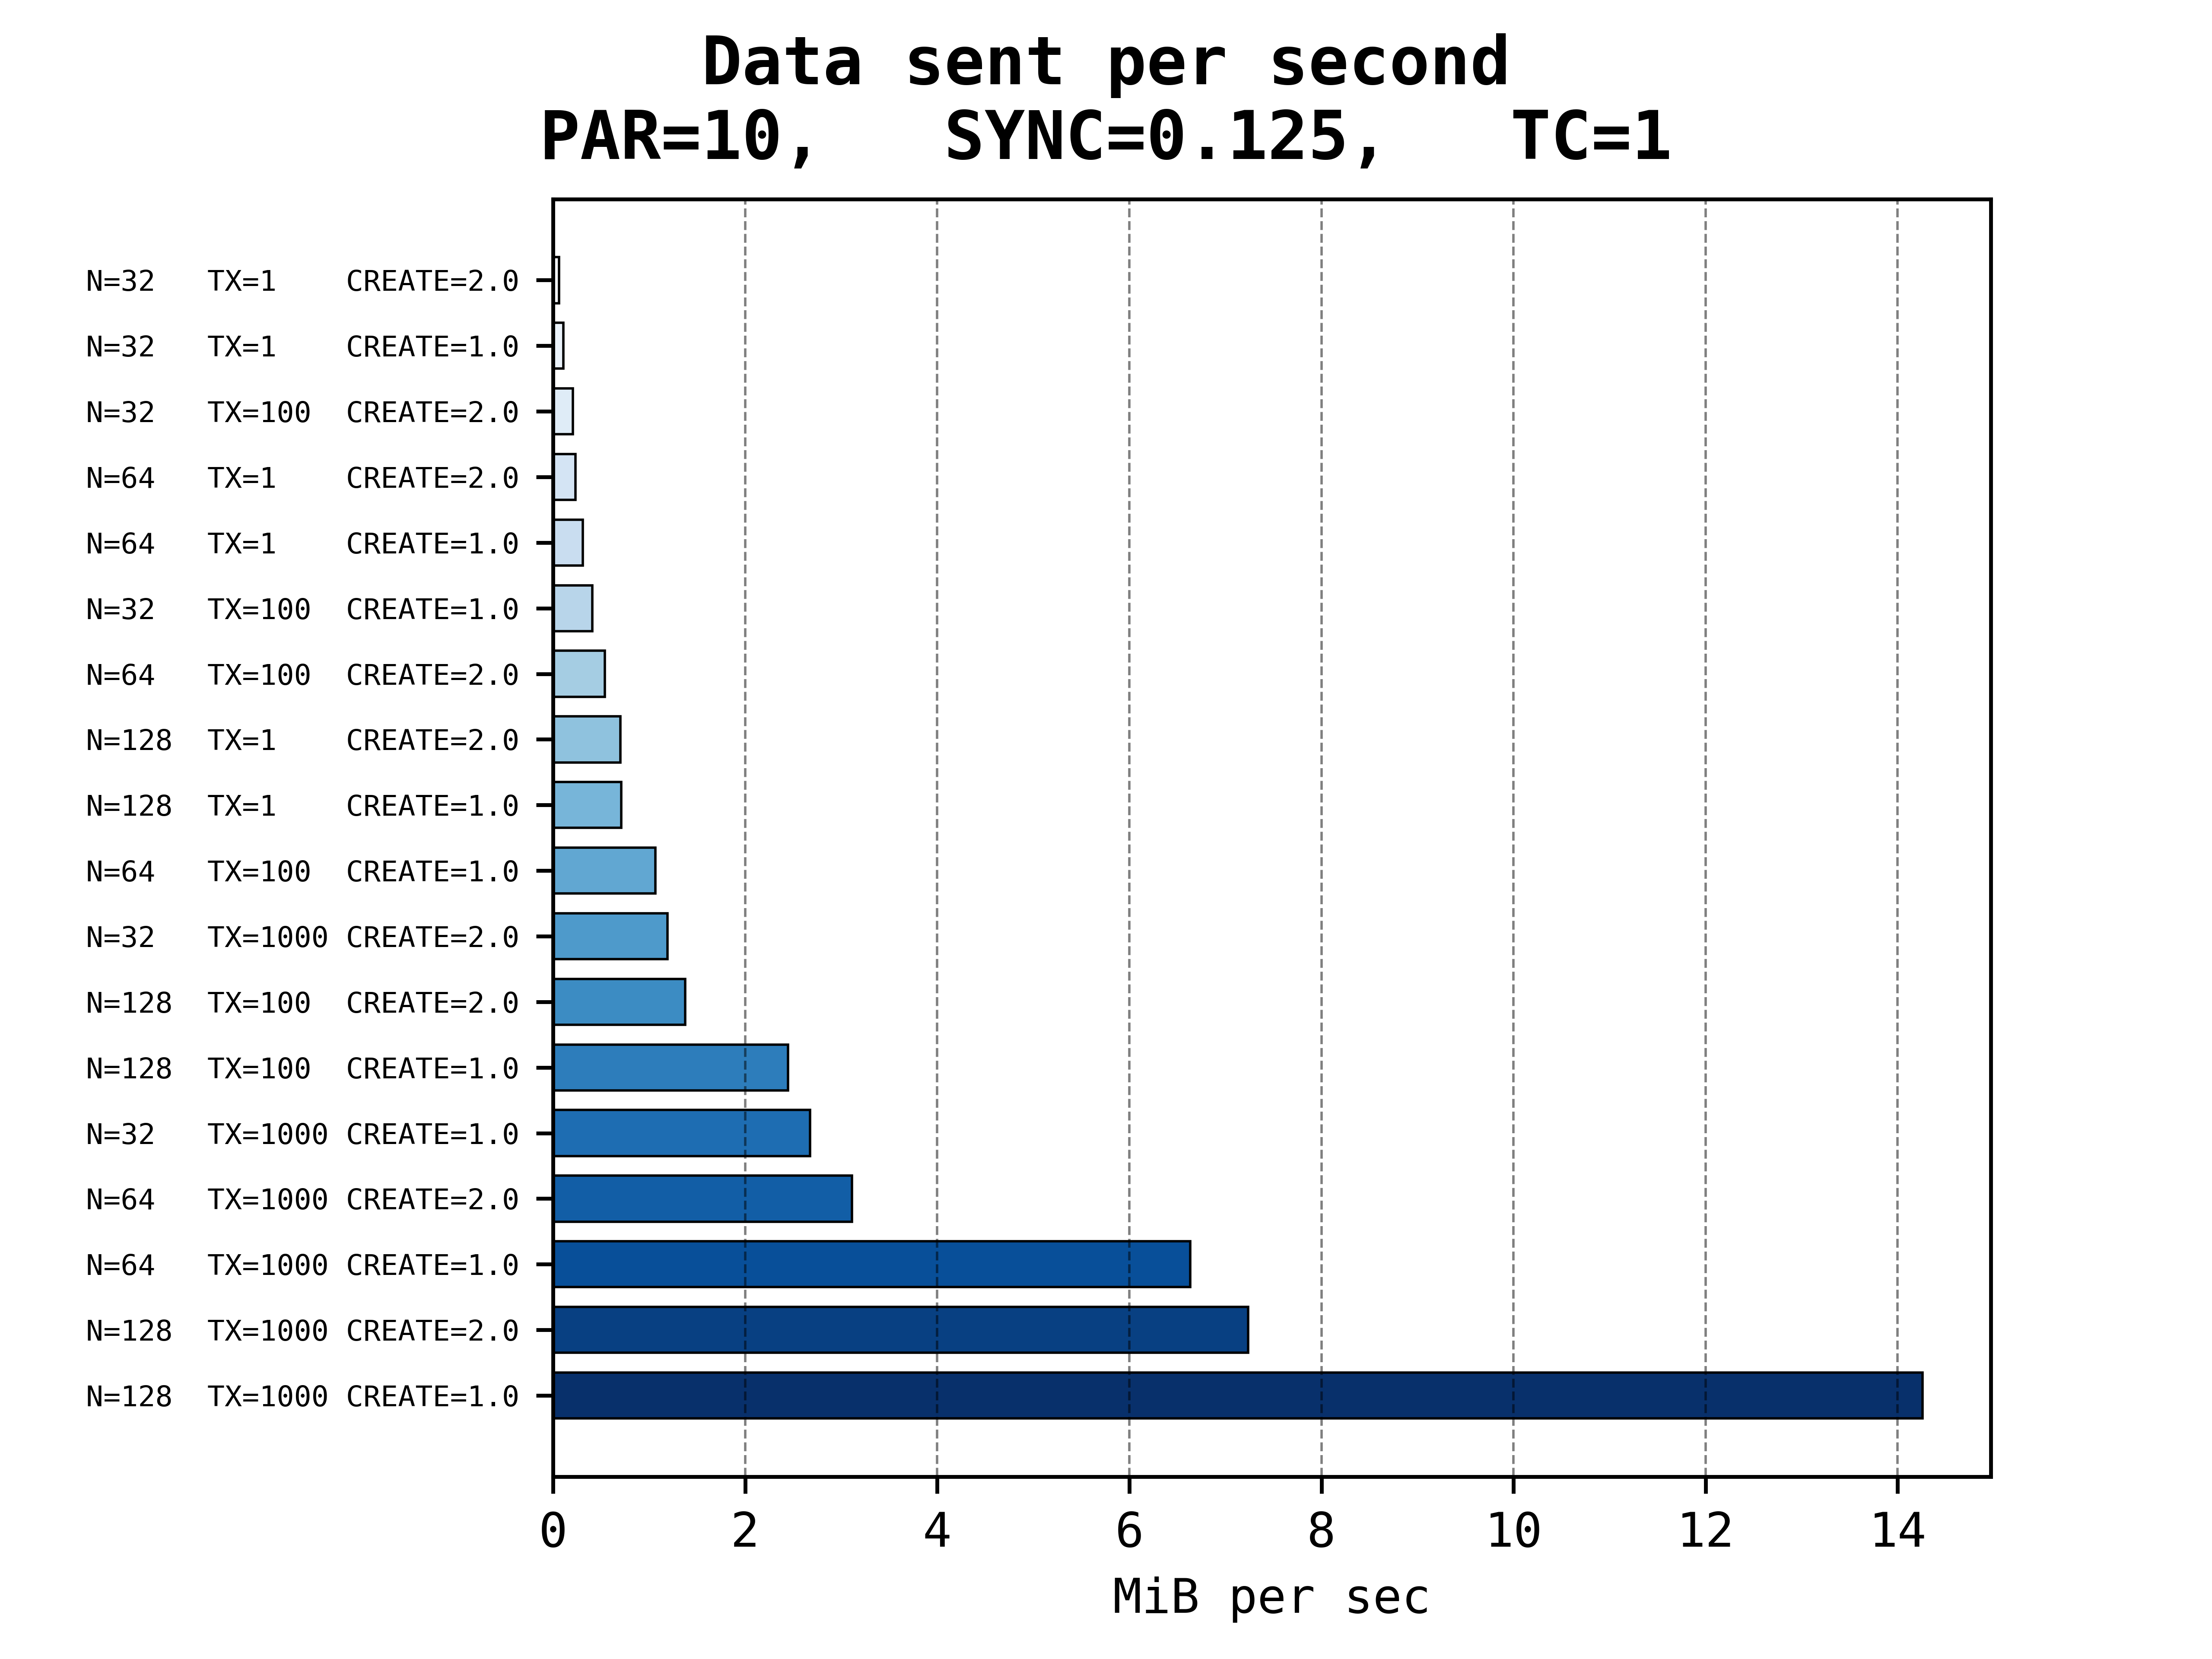
\includegraphics[width=0.8\textwidth]{bar_plots/final_exp2/bytes_sent_per_sec.png}
				\caption{The average amount of data sent per second.}
				\label{fig:transactionsBps}
			\end{figure}
		\FloatBarrier
		\subsection{Committee size}
		\FloatBarrier
		The last series of experiments was designed to test Aleph's scaling with committee size, but also check the necessity of parent restrictions.
		There were two major differences with respect to previous tests.
		We used a simple adaptive create delay algorithm, that lowered the delay if a unit was created on a new level twice in a row and increased it if a unit was created at the same level as the previous one.
		This means the create delays in the graphs are only initial values.
		The creation algorithm used has changed too -- in this series we used the newer algorithm described in Section \ref{sec:creation}.
		We also ran the tests for $50$ levels, in contrast to the previous tests where the limit was $20$.
			\begin{figure}[h]
				\centering
				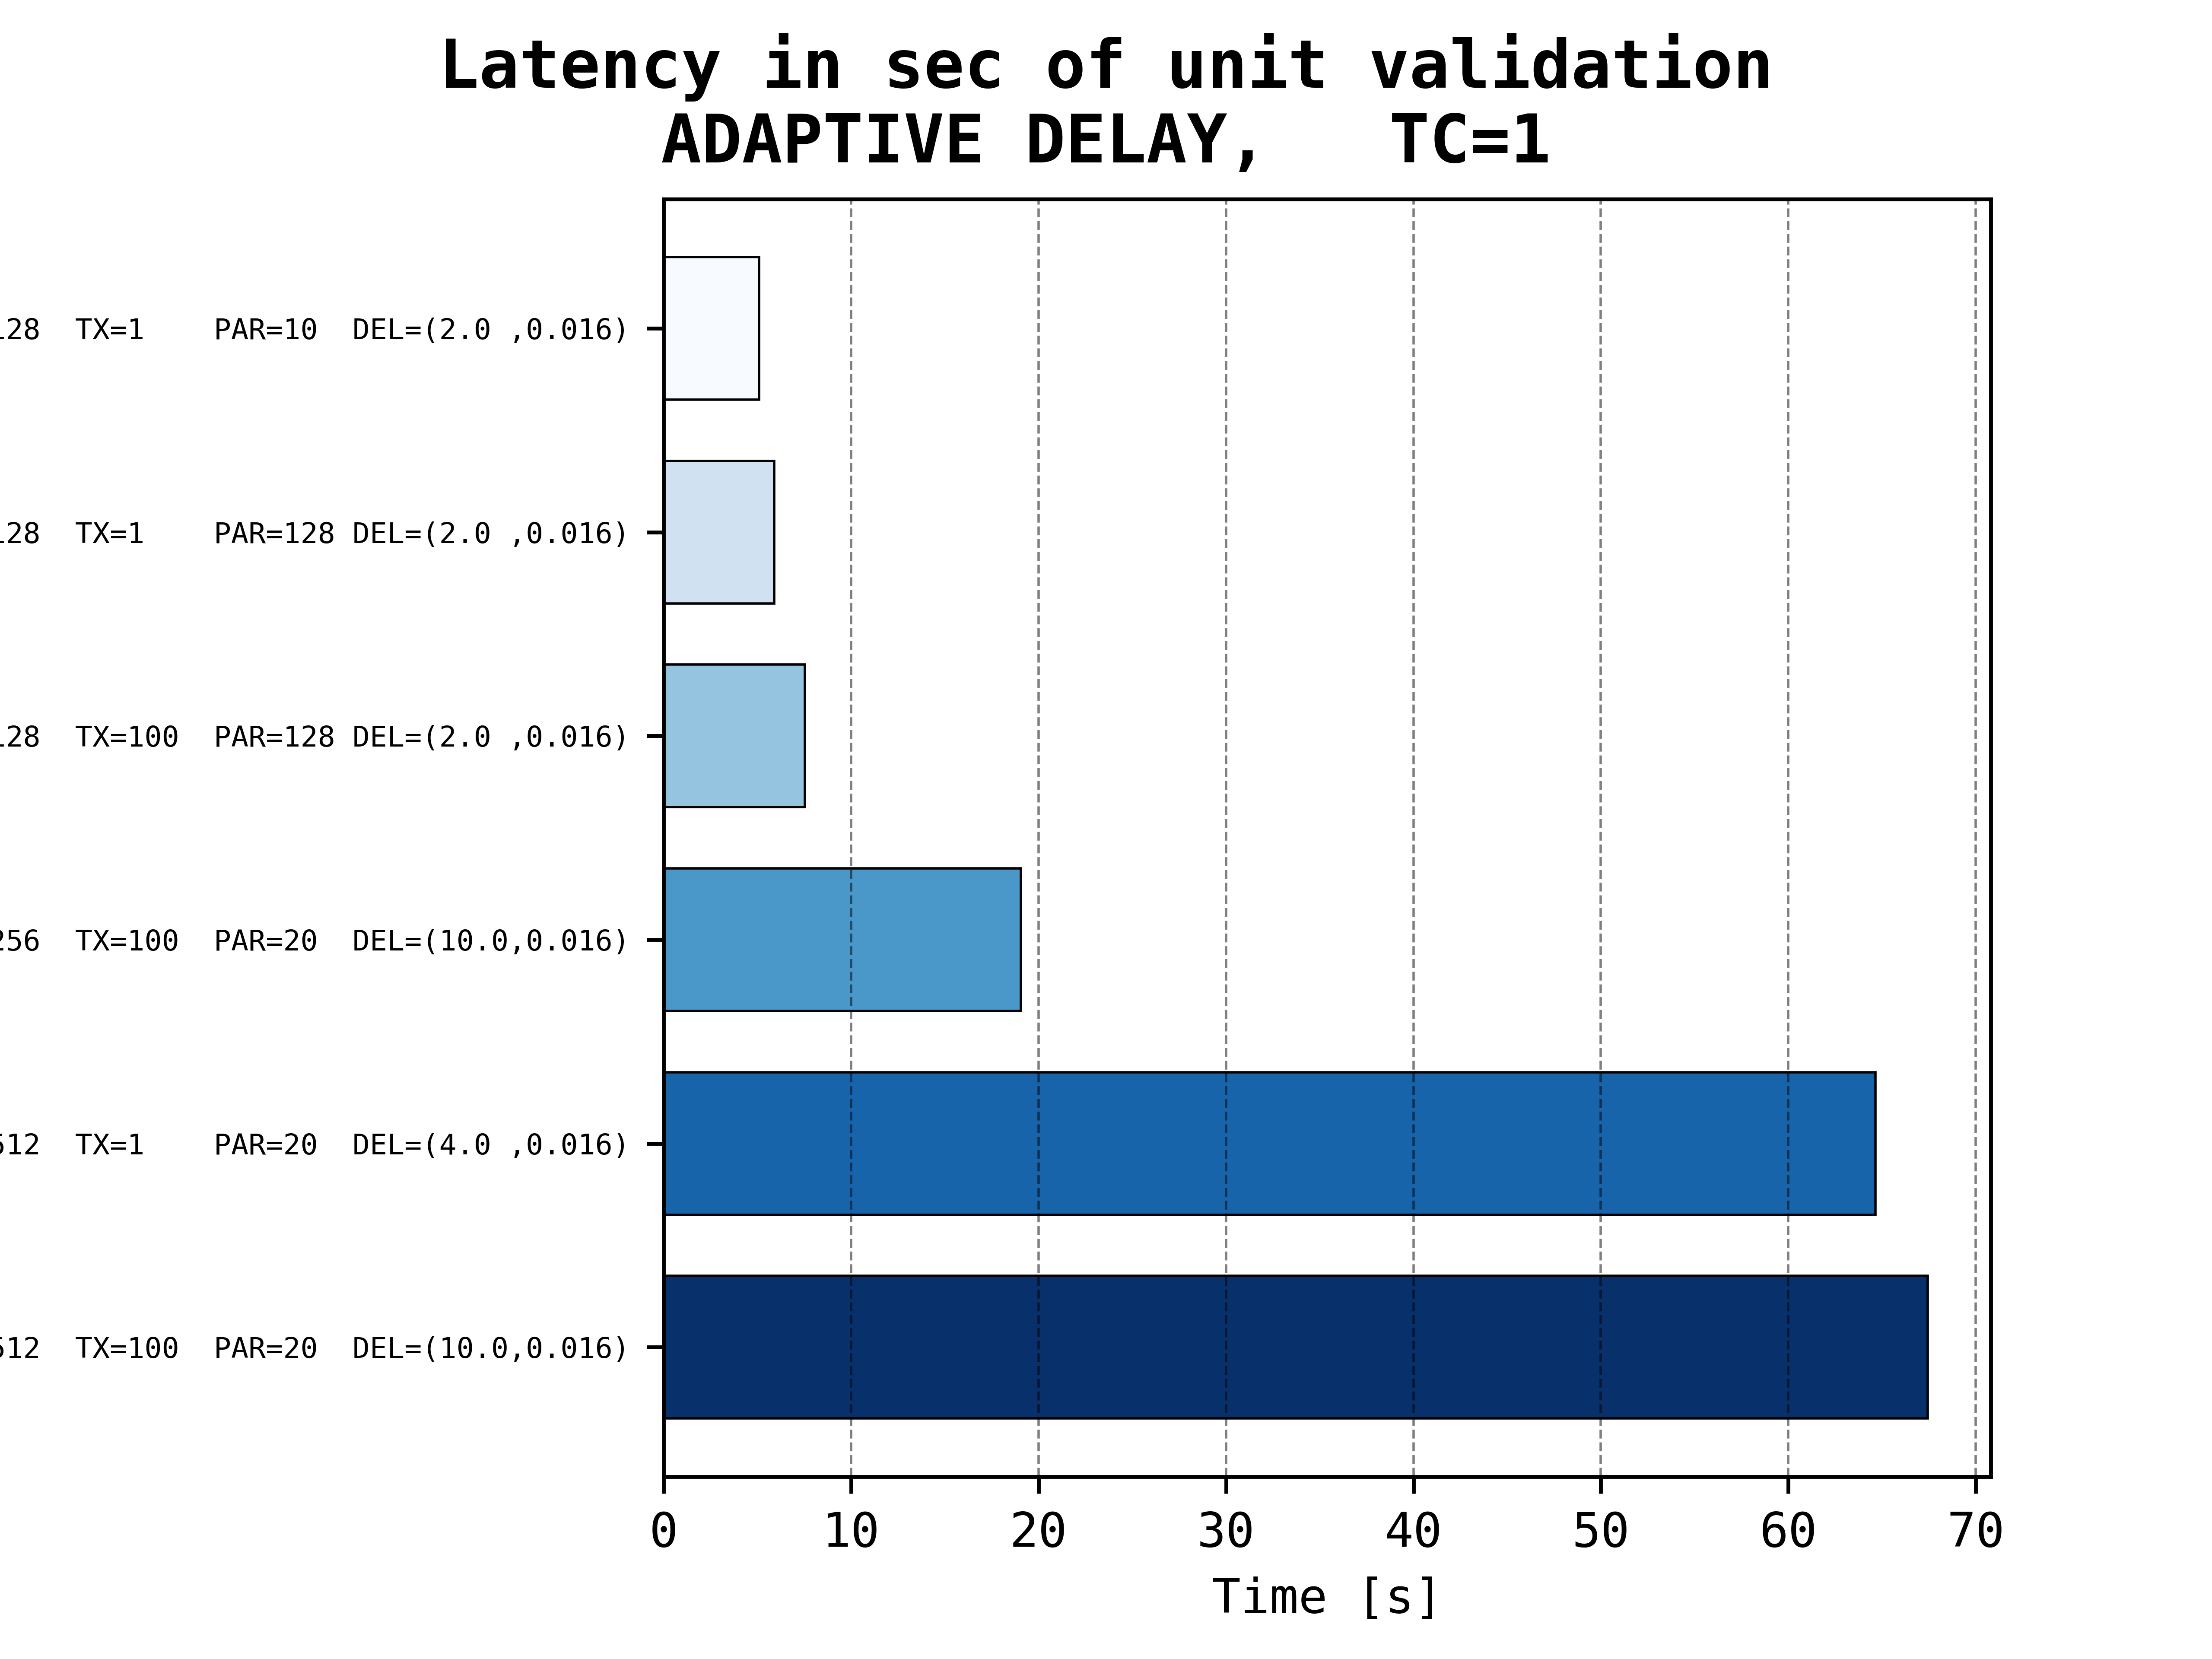
\includegraphics[width=0.8\textwidth]{bar_plots/big/create_ord_del.png}
				\caption{The latency of unit validation in the last series of experiments.}
				\label{fig:bigLatency}
			\end{figure}
			\begin{figure}[h]
				\centering
				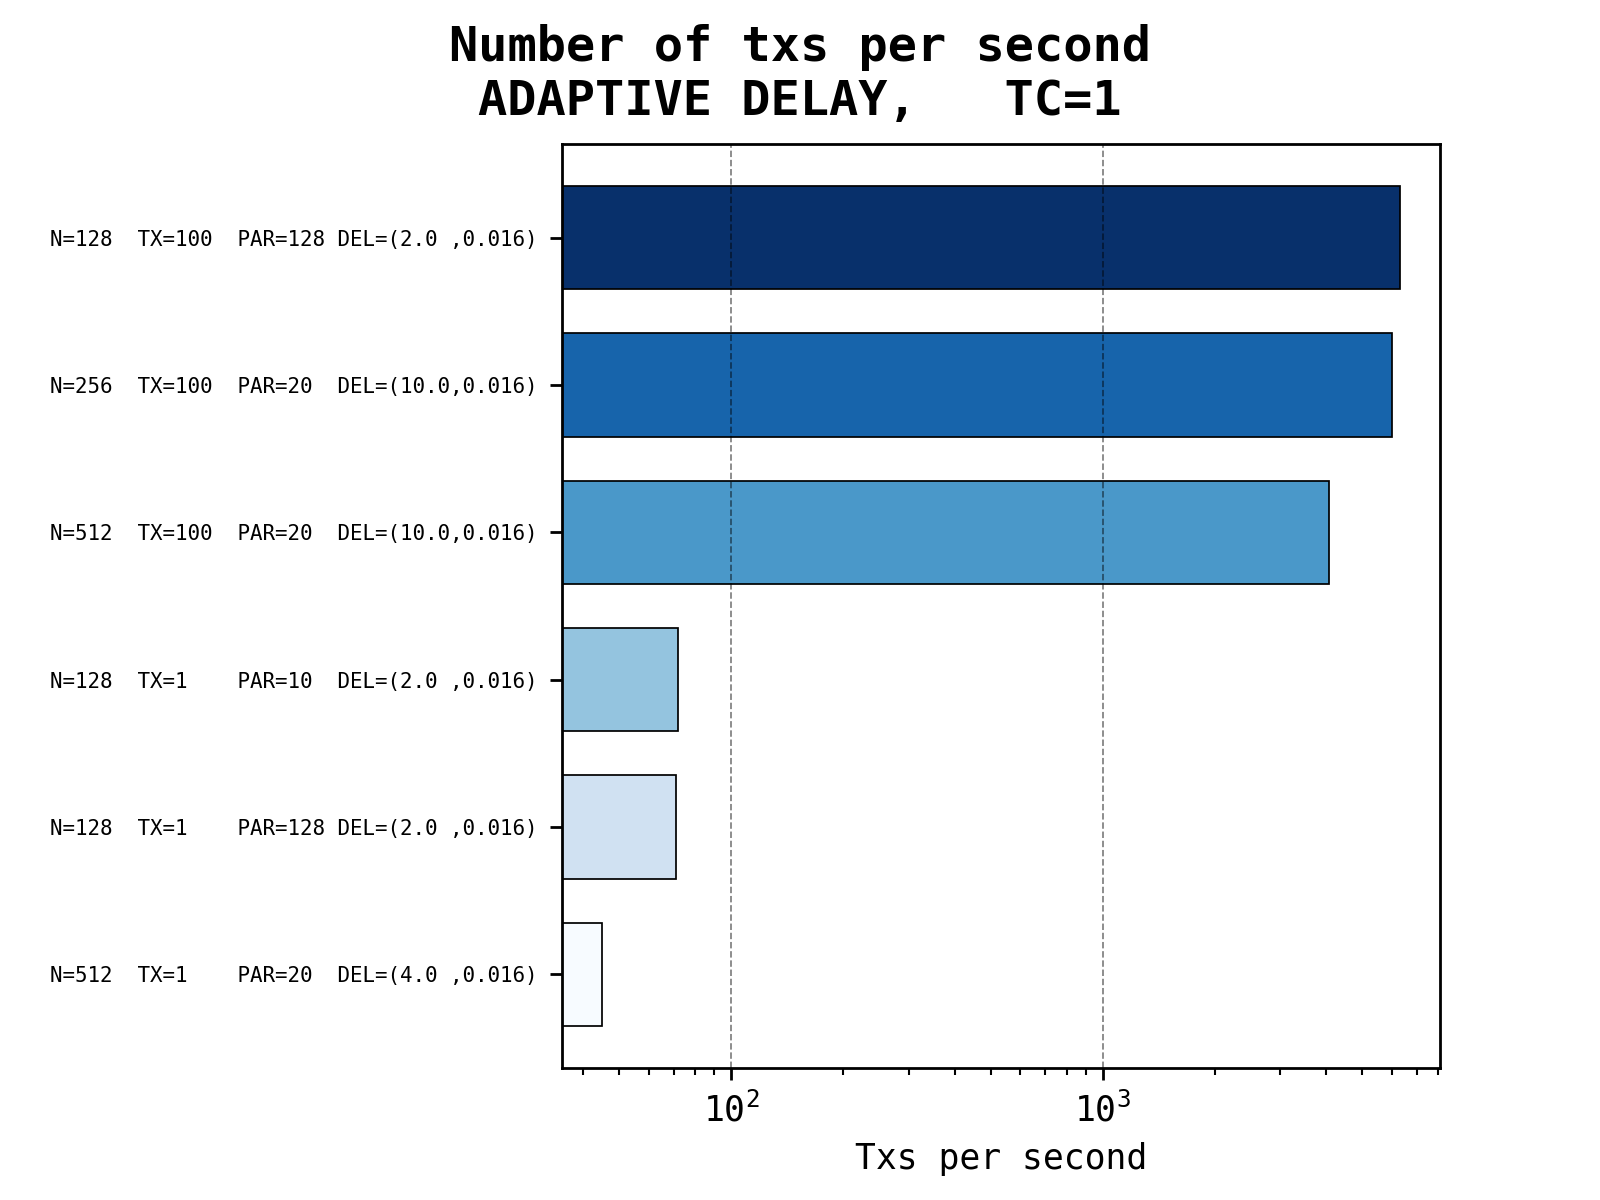
\includegraphics[width=0.8\textwidth]{bar_plots/big/txps.png}
				\caption{The number of transaction entering the system per second.}
				\label{fig:bigTxps}
			\end{figure}
			\begin{figure}[h]
				\centering
				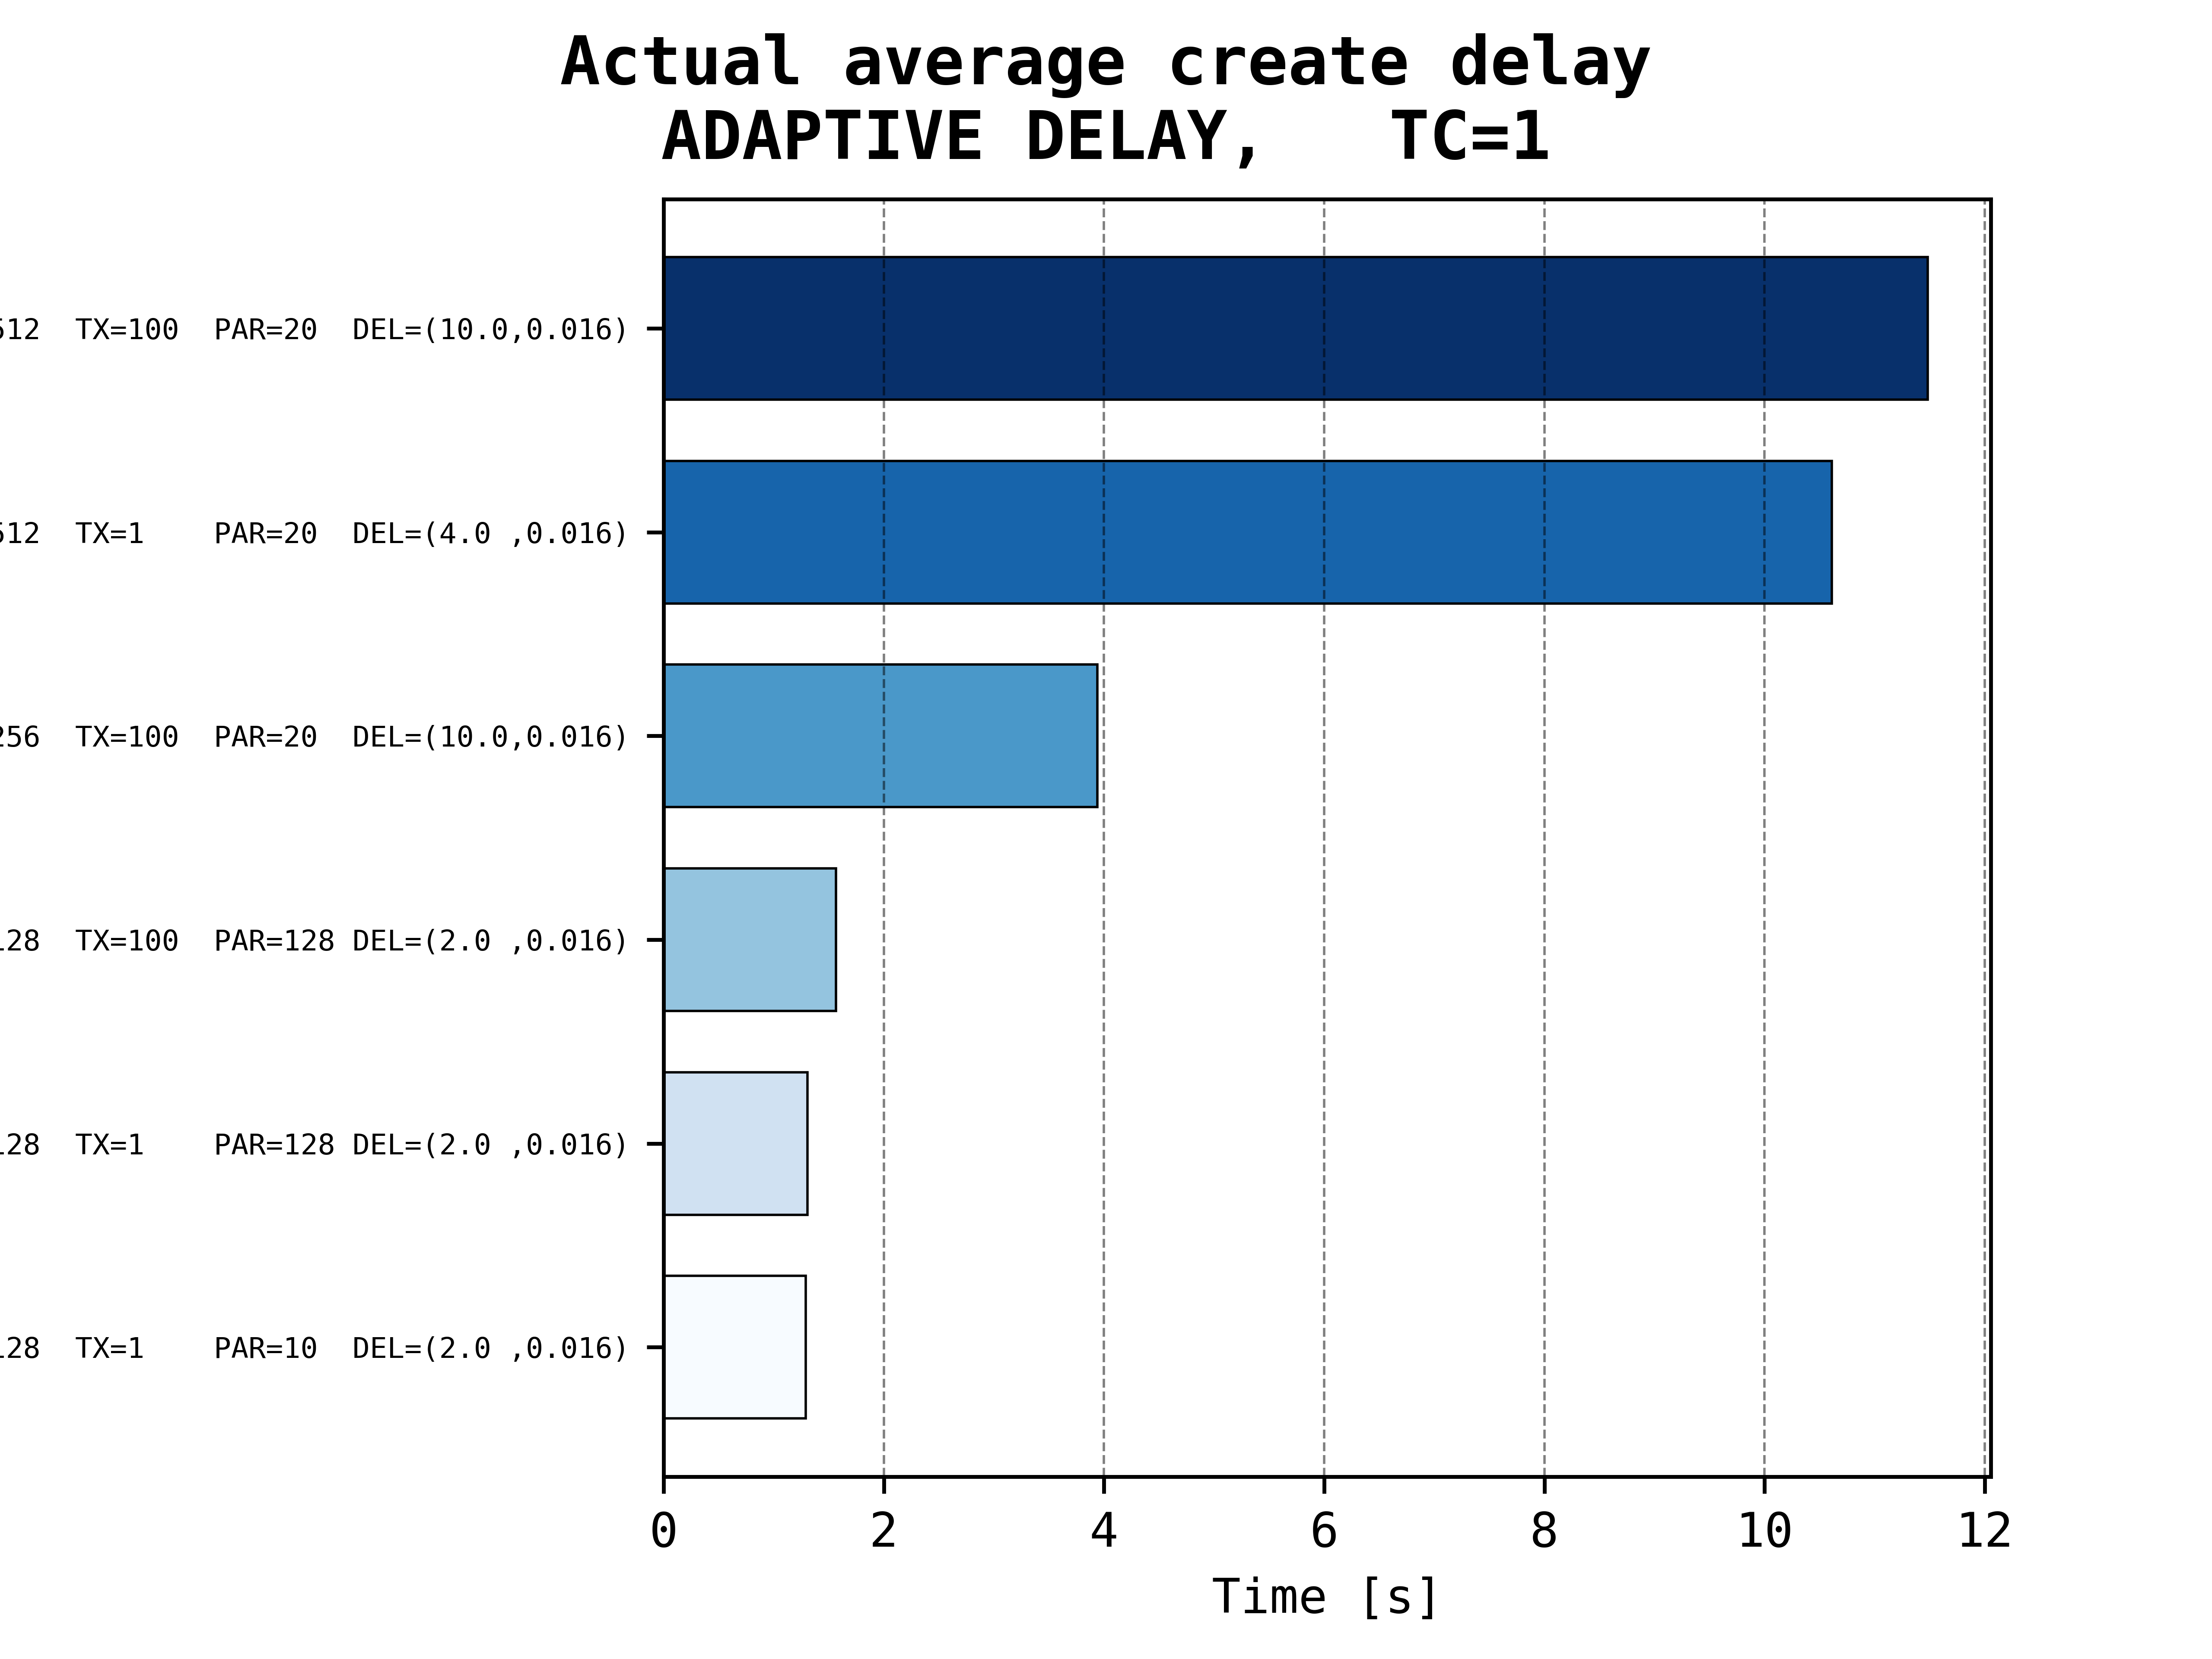
\includegraphics[width=0.8\textwidth]{bar_plots/big/create_delay.png}
				\caption{The time between unit creation attempts. This reflects the adaptive value quite well.}
				\label{fig:bigCreateDelay}
			\end{figure}
			\begin{figure}[h]
				\centering
				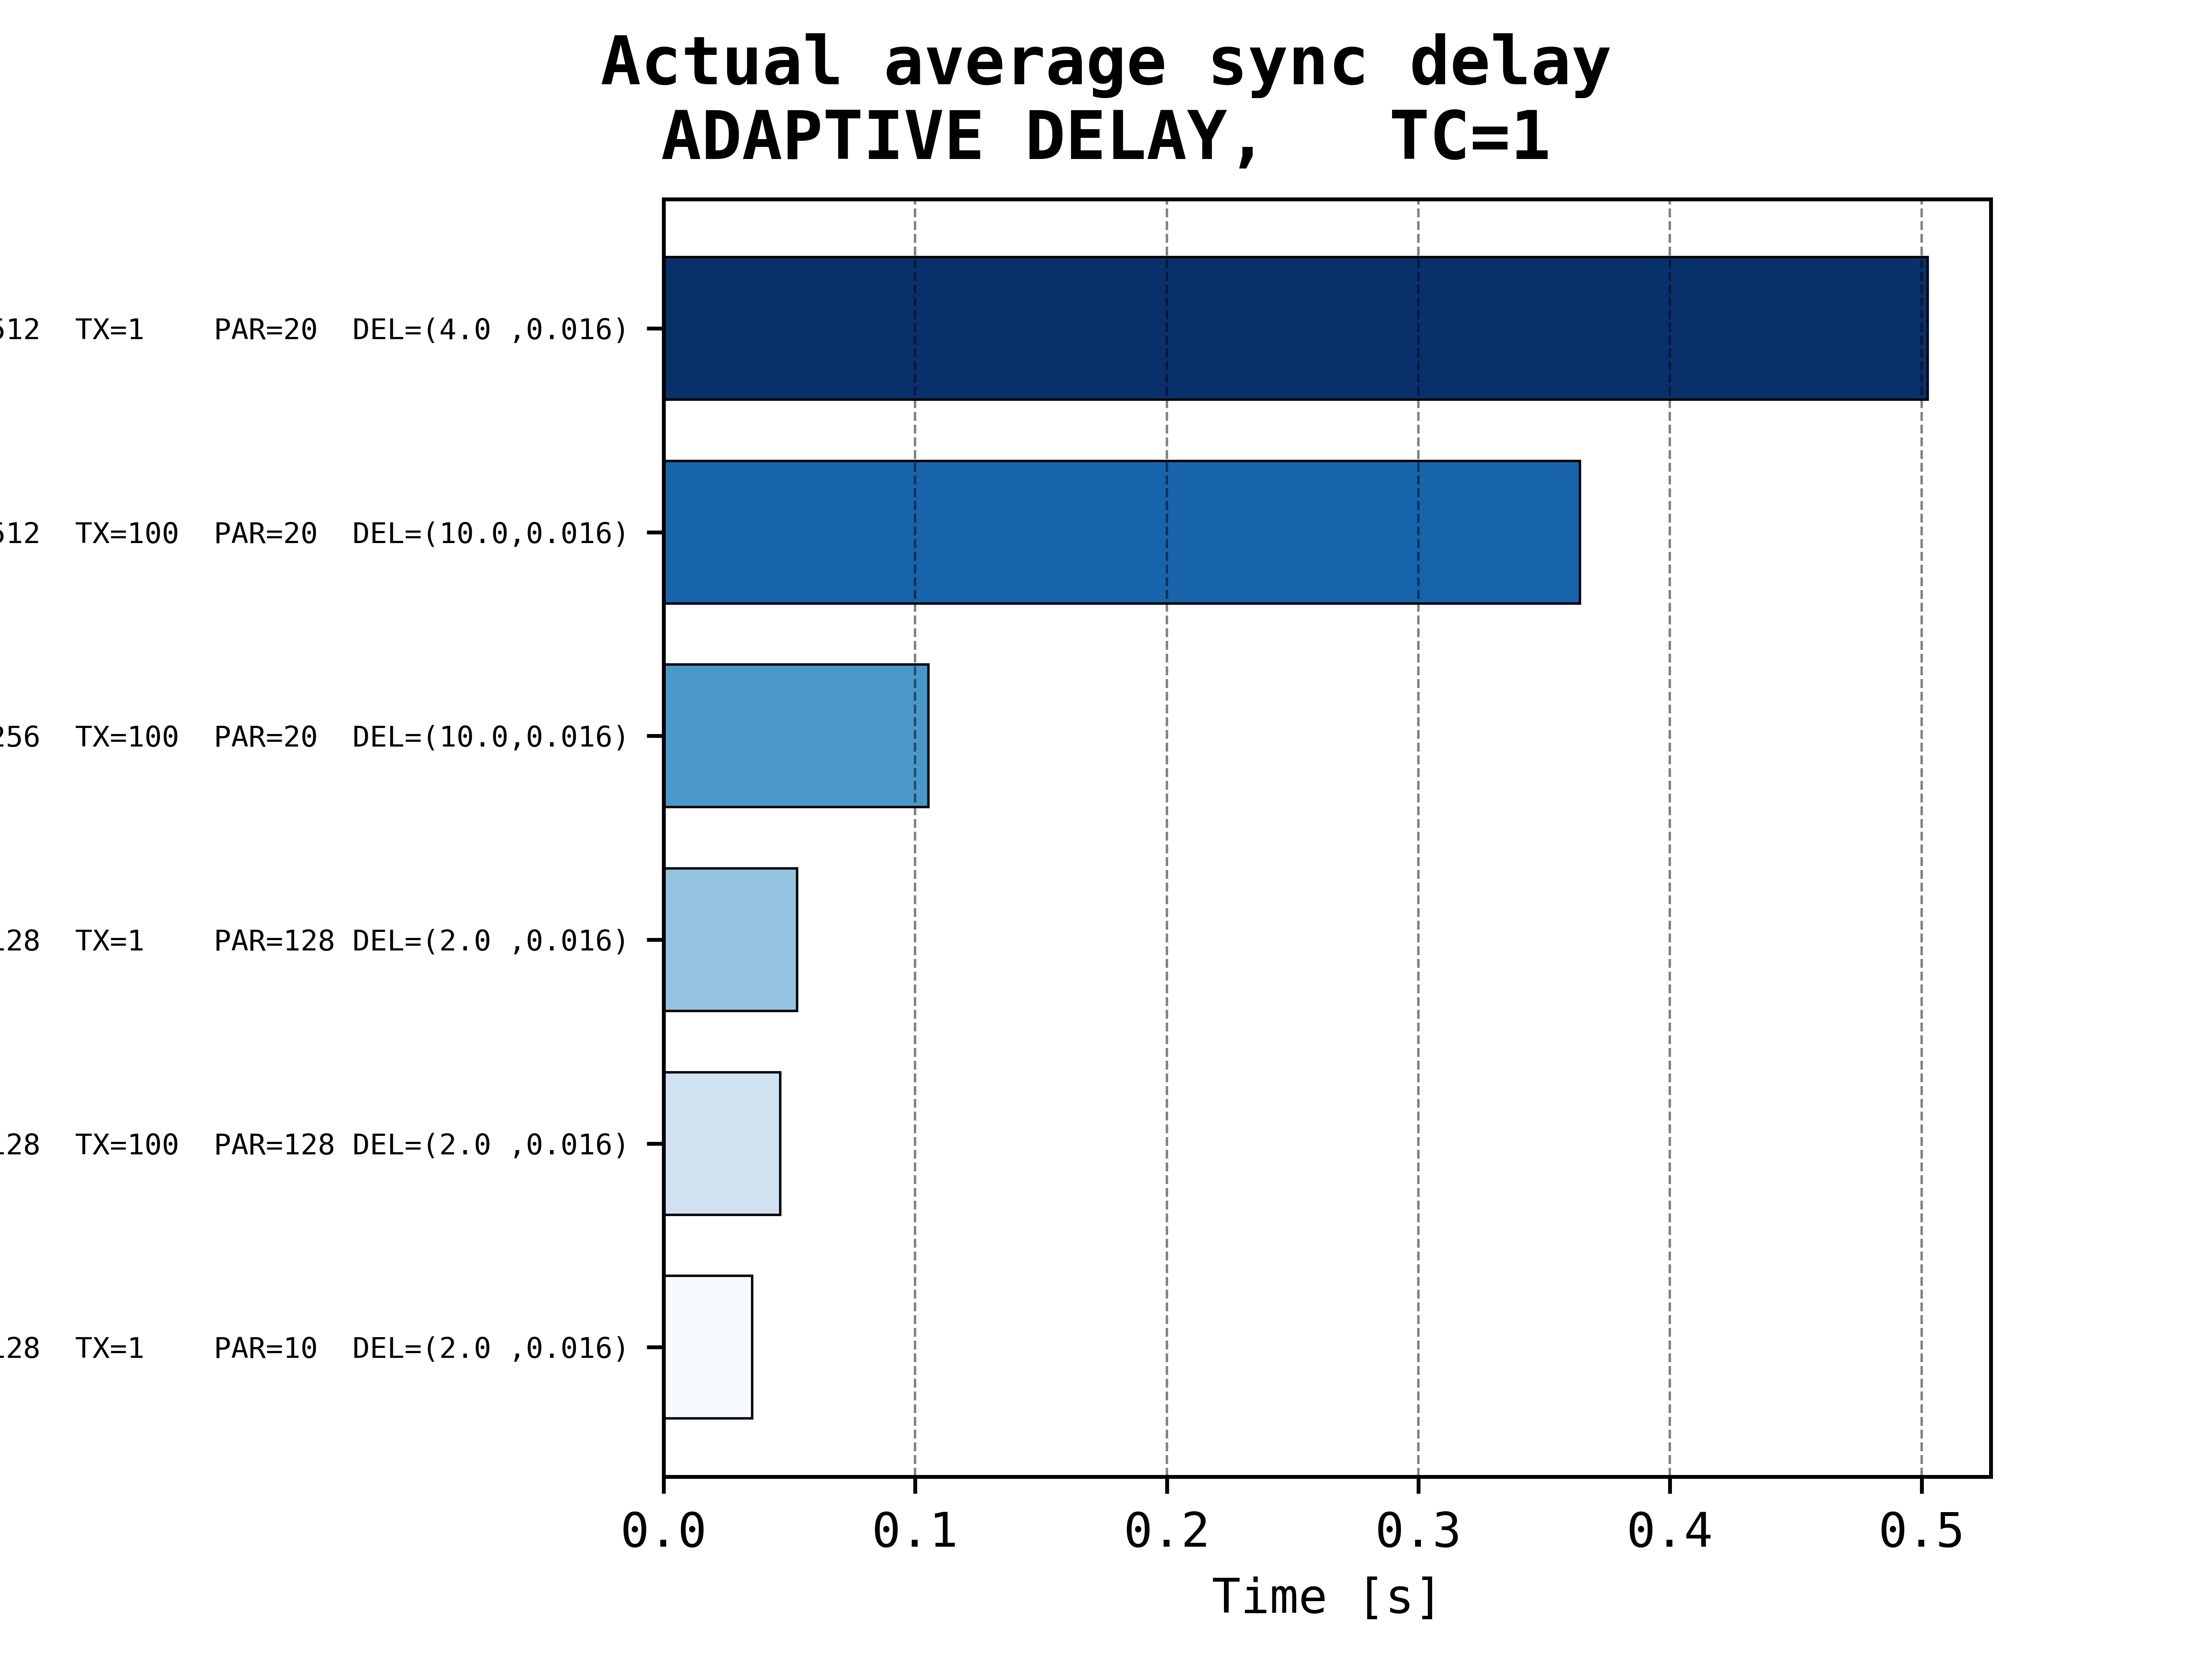
\includegraphics[width=0.8\textwidth]{bar_plots/big/sync_delay.png}
				\caption{The time between sync attempts.}
				\label{fig:bigSyncDelay}
			\end{figure}
			\begin{figure}[h]
				\centering
				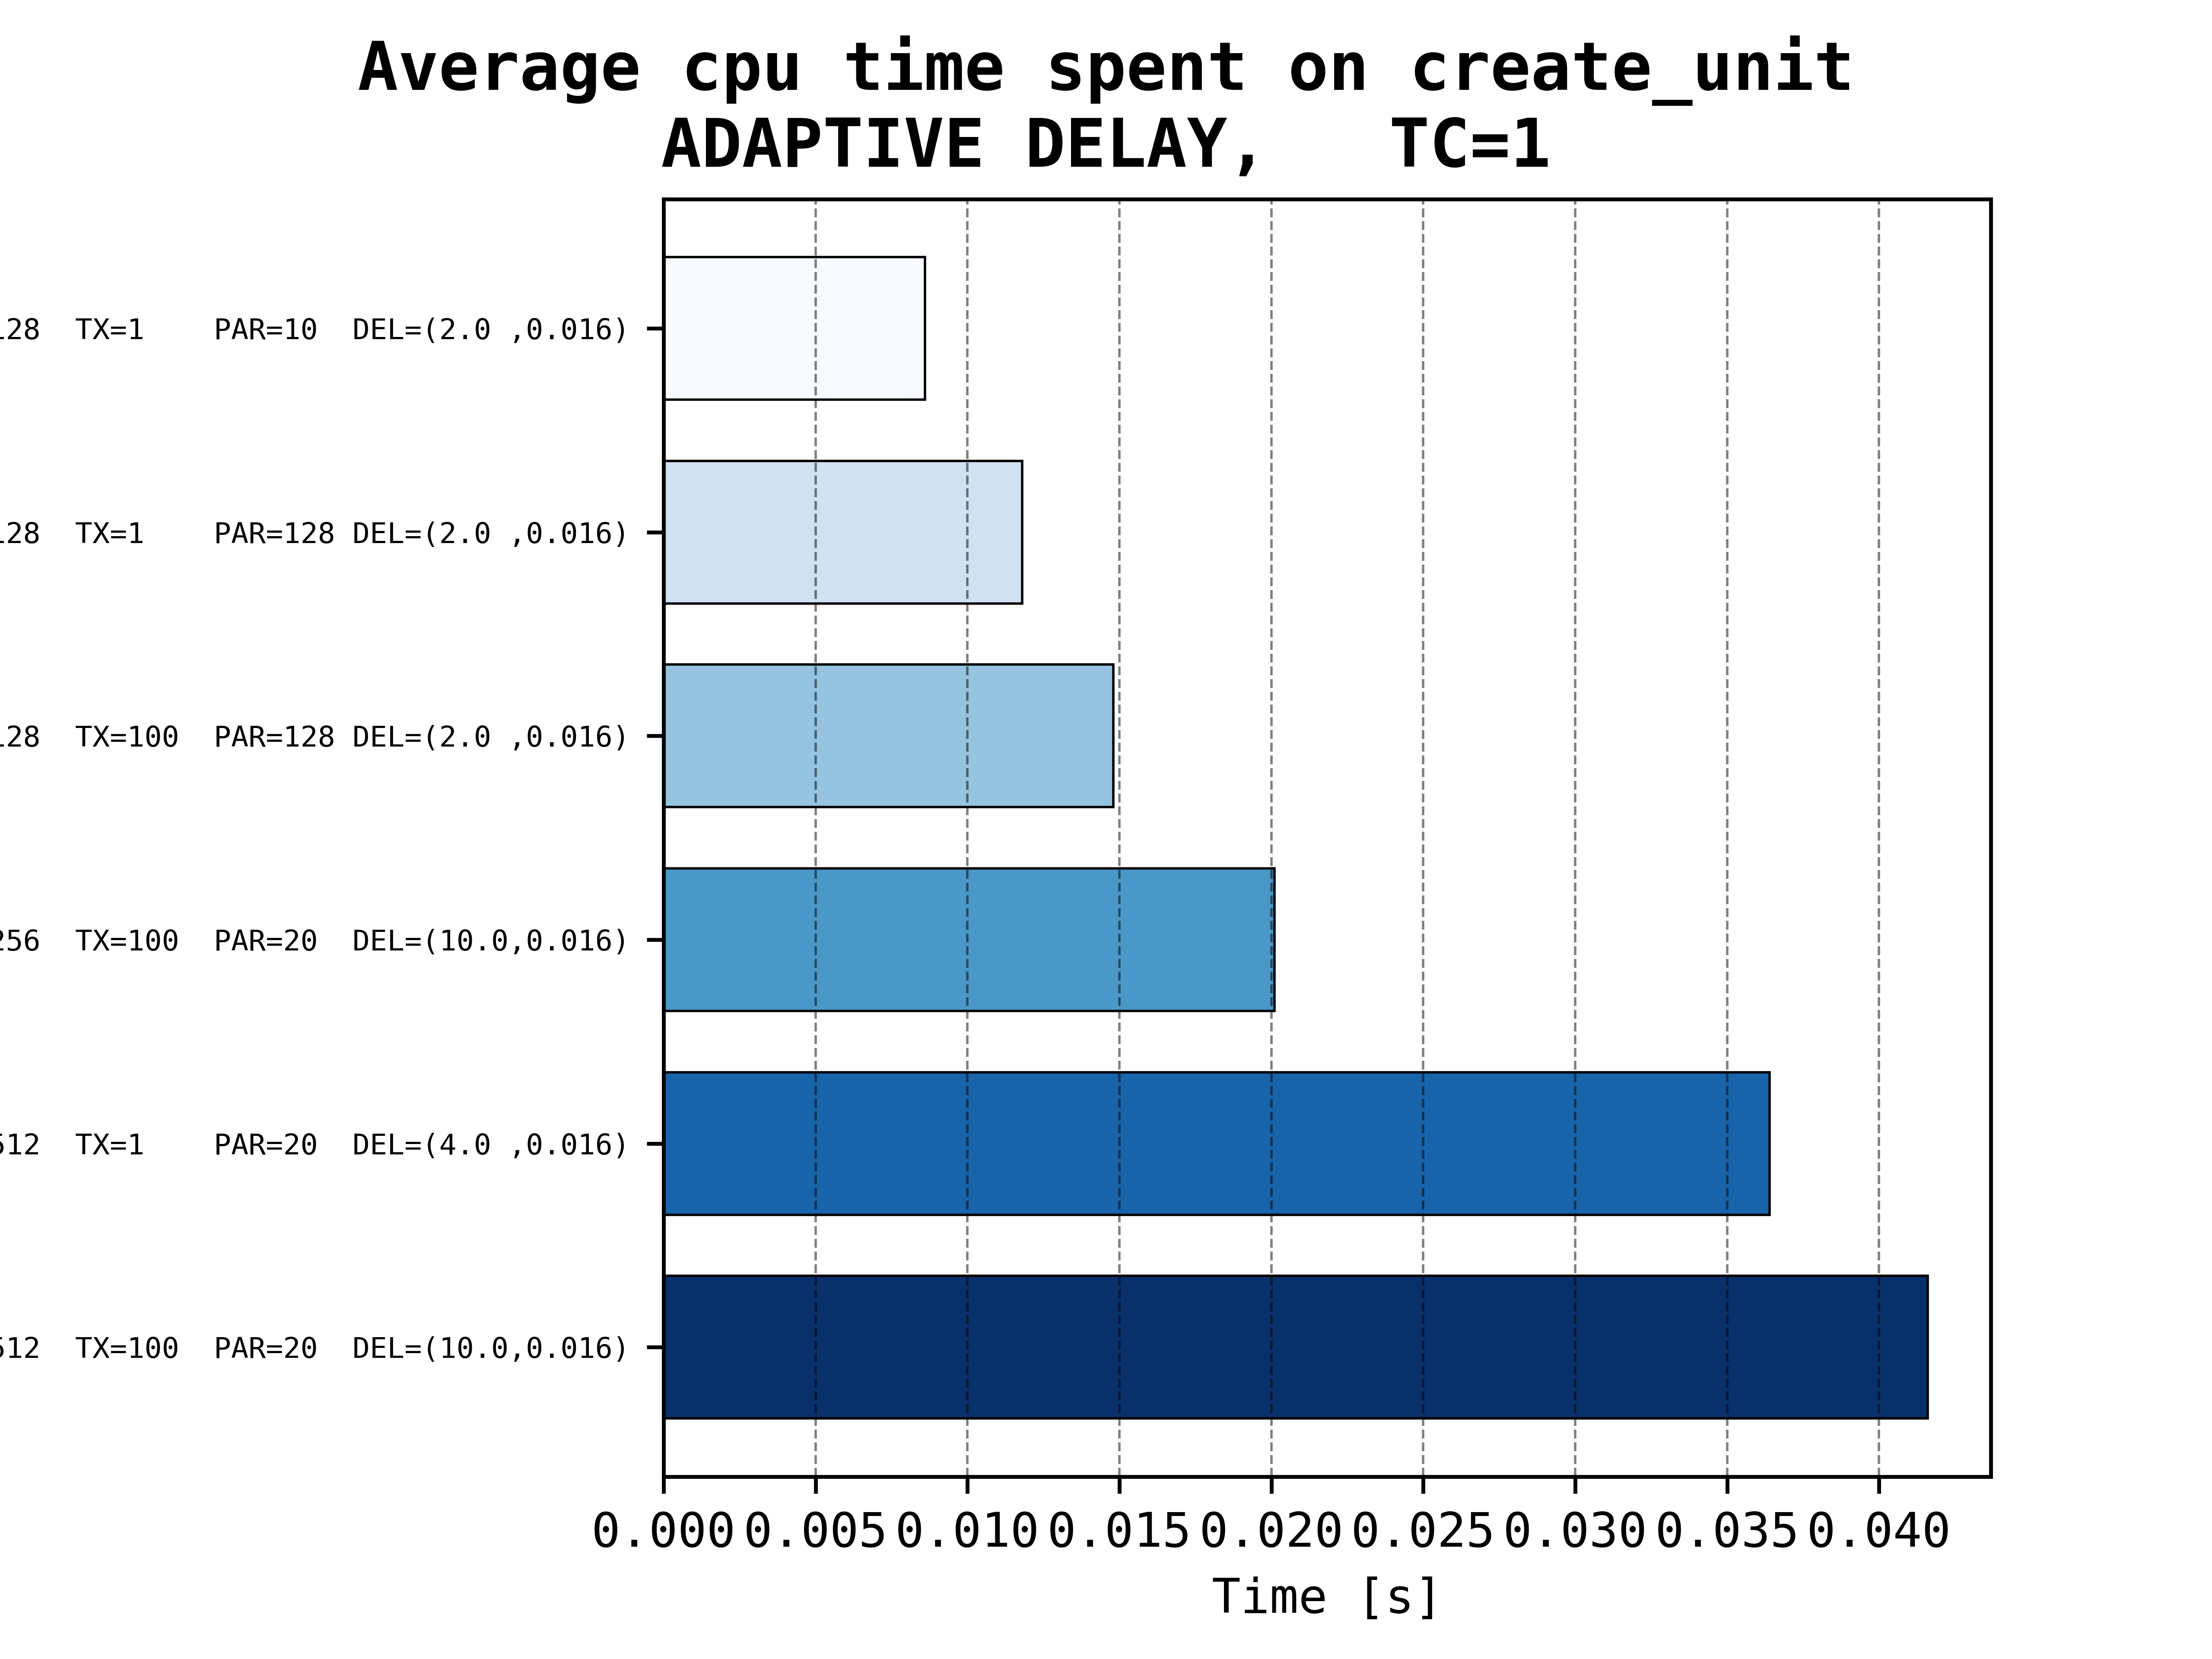
\includegraphics[width=0.8\textwidth]{bar_plots/big/time_create.png}
				\caption{The average time it took to create a unit. Note the difference when parents were unrestricted.}
				\label{fig:bigTimeCreate}
			\end{figure}
			\begin{figure}[h]
				\centering
				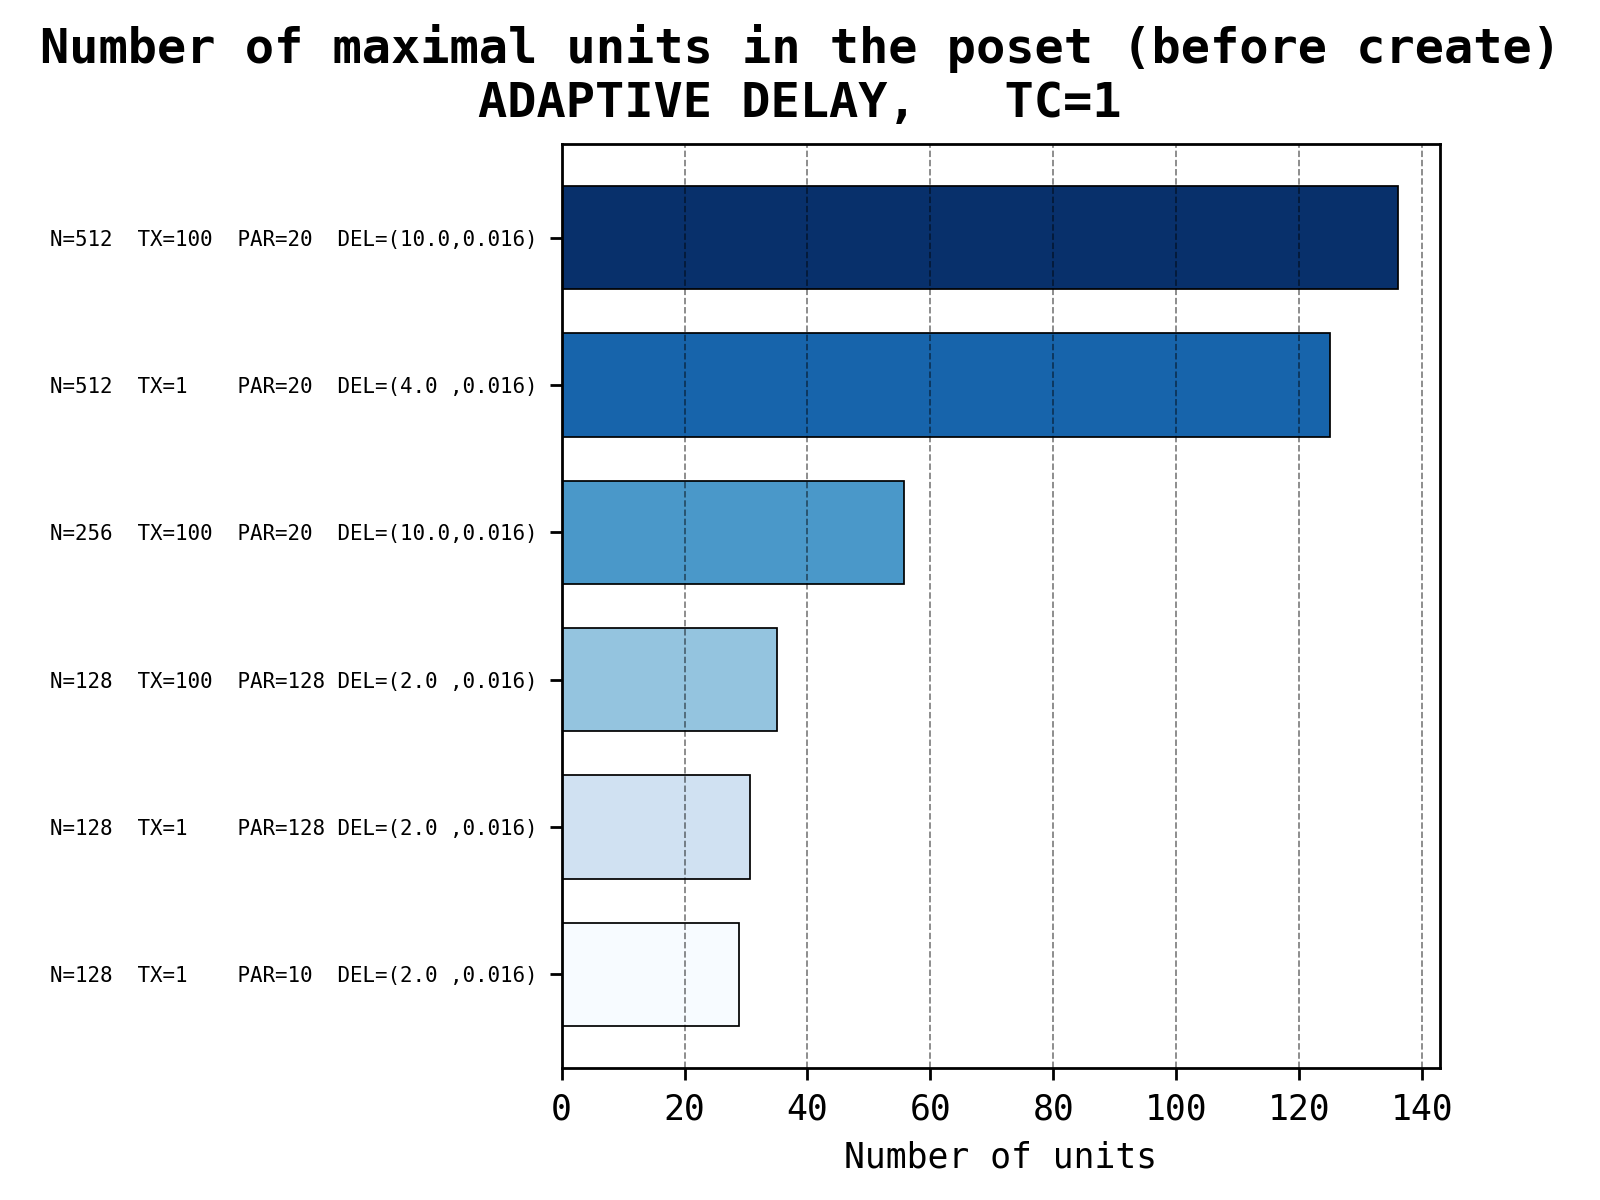
\includegraphics[width=0.8\textwidth]{bar_plots/big/n_maximal.png}
				\caption{Number of maximal units in the poset before a create.}
				\label{fig:bigMaximalPreCreate}
			\end{figure}
			\begin{figure}[h]
				\centering
				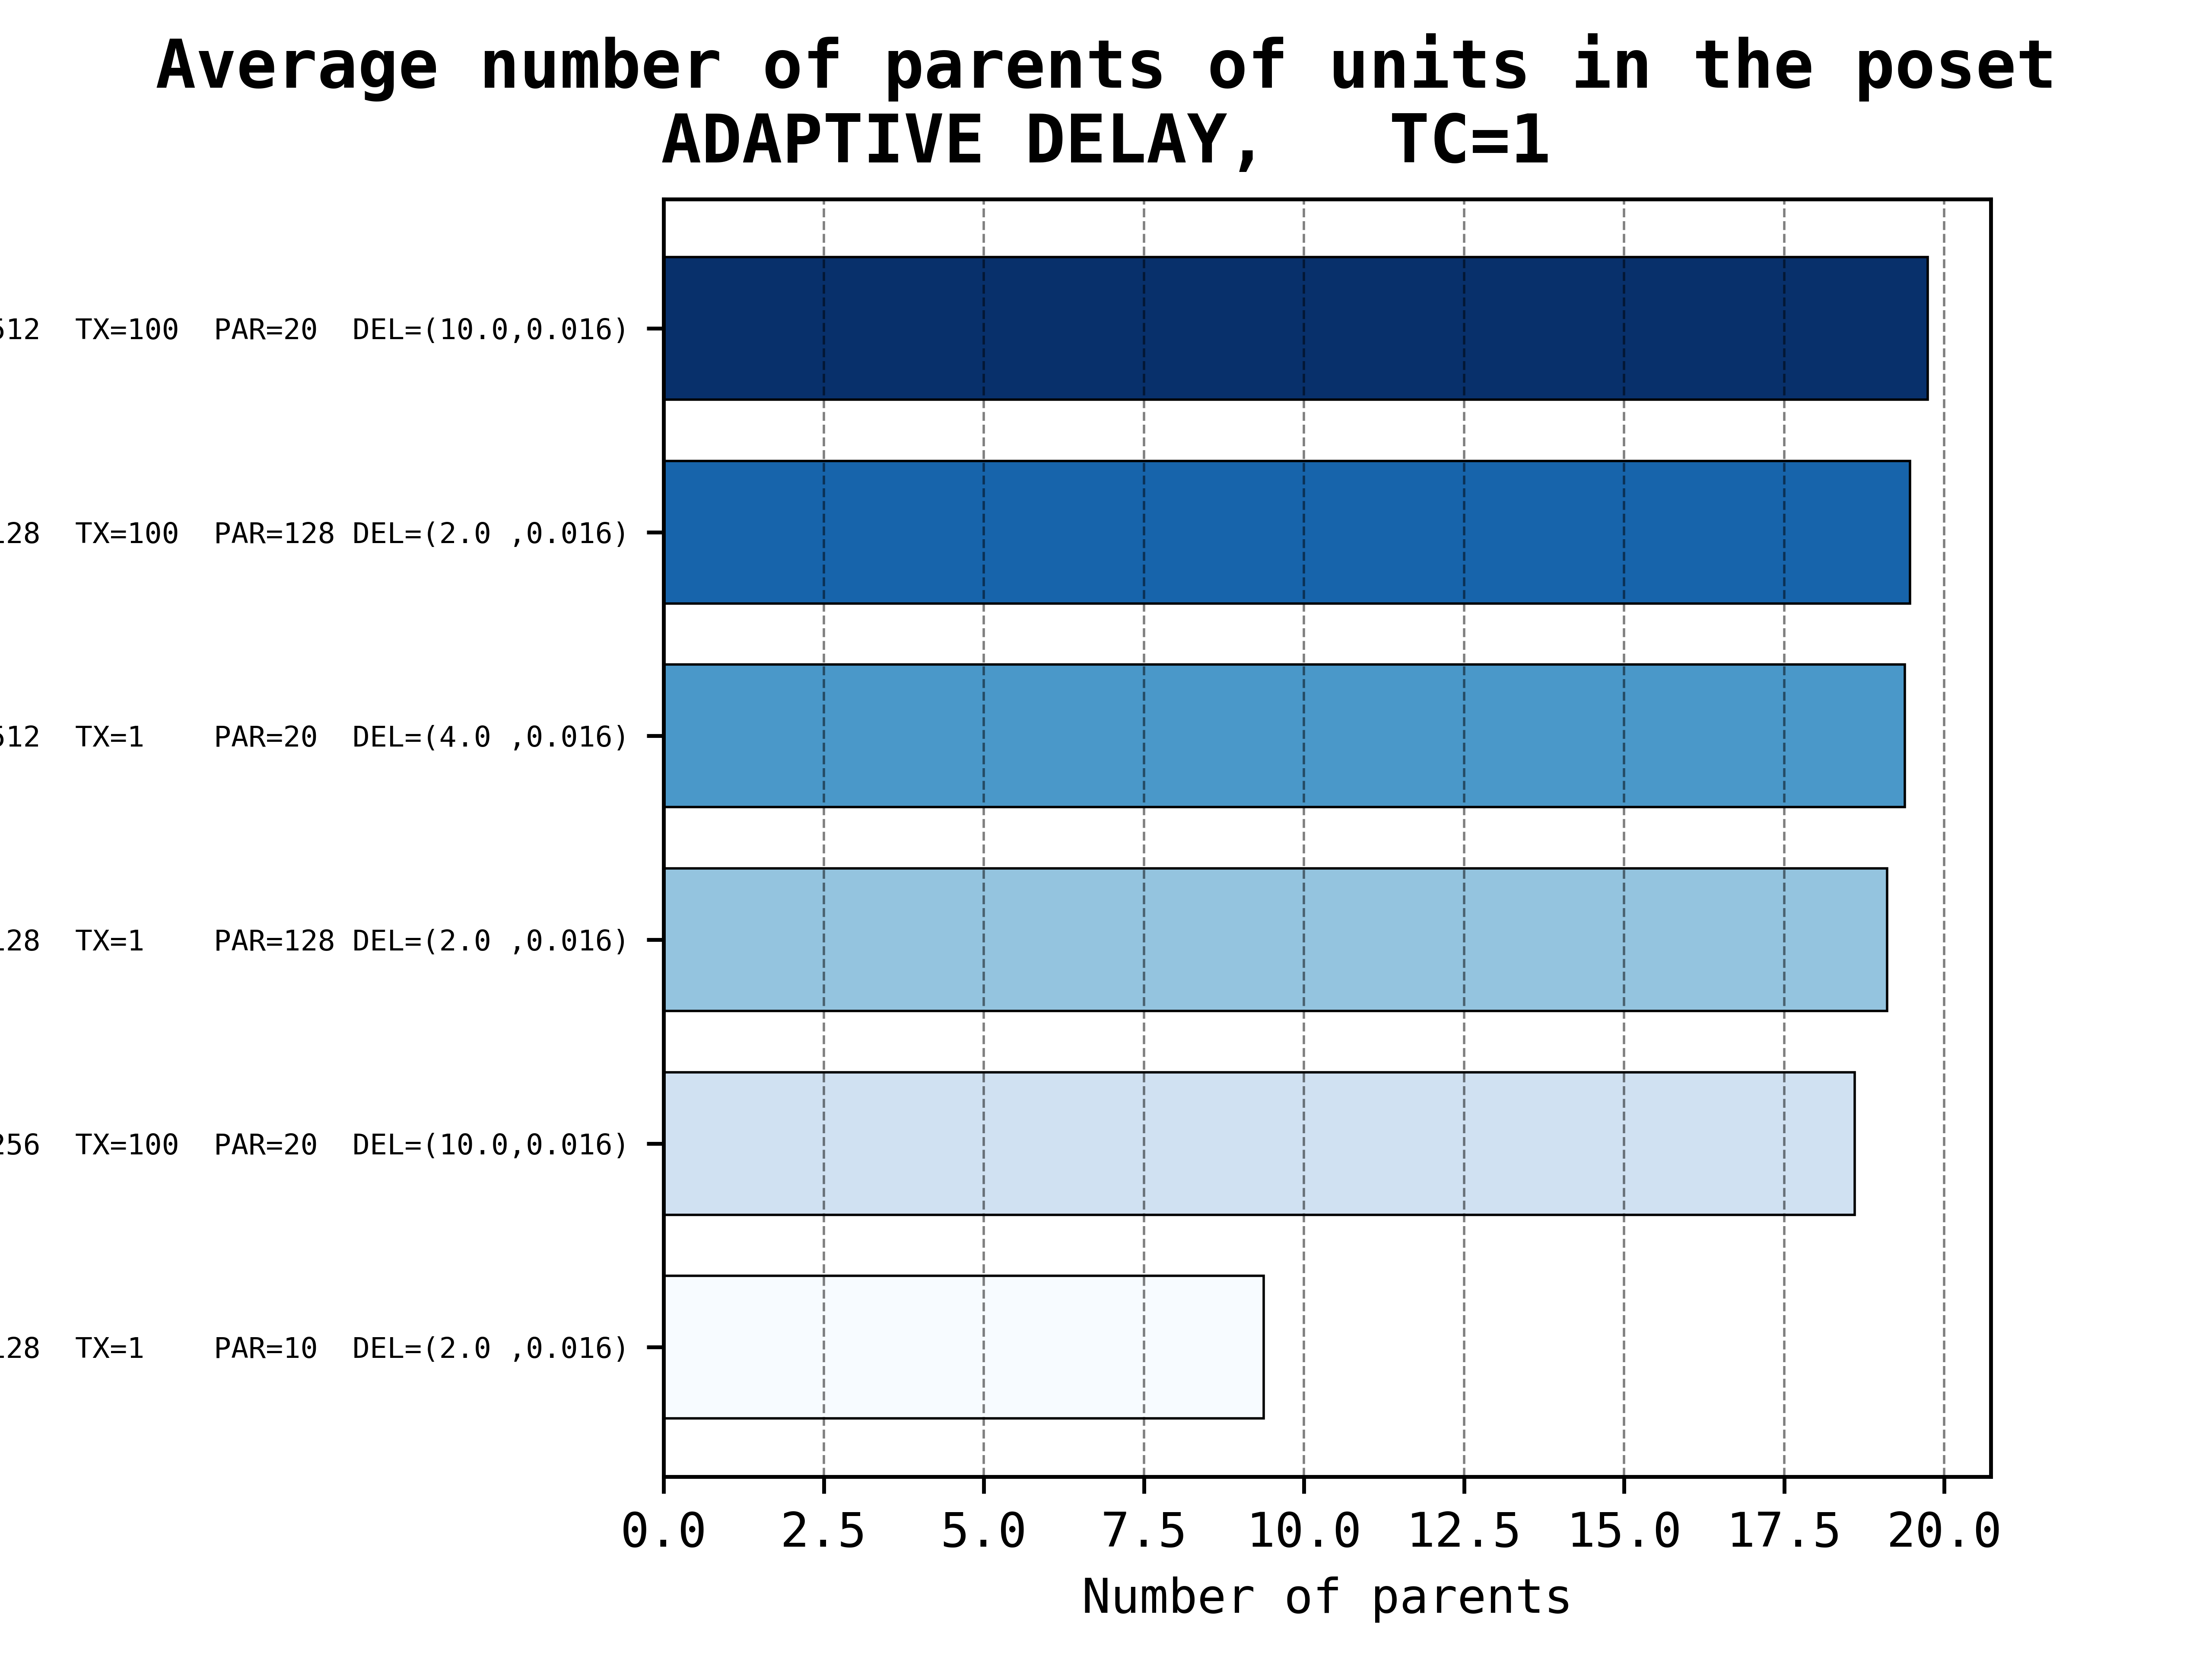
\includegraphics[width=0.8\textwidth]{bar_plots/big/n_parents.png}
				\caption{The average number of parents per unit.}
				\label{fig:bigParents}
			\end{figure}
			\begin{figure}[h]
				\centering
				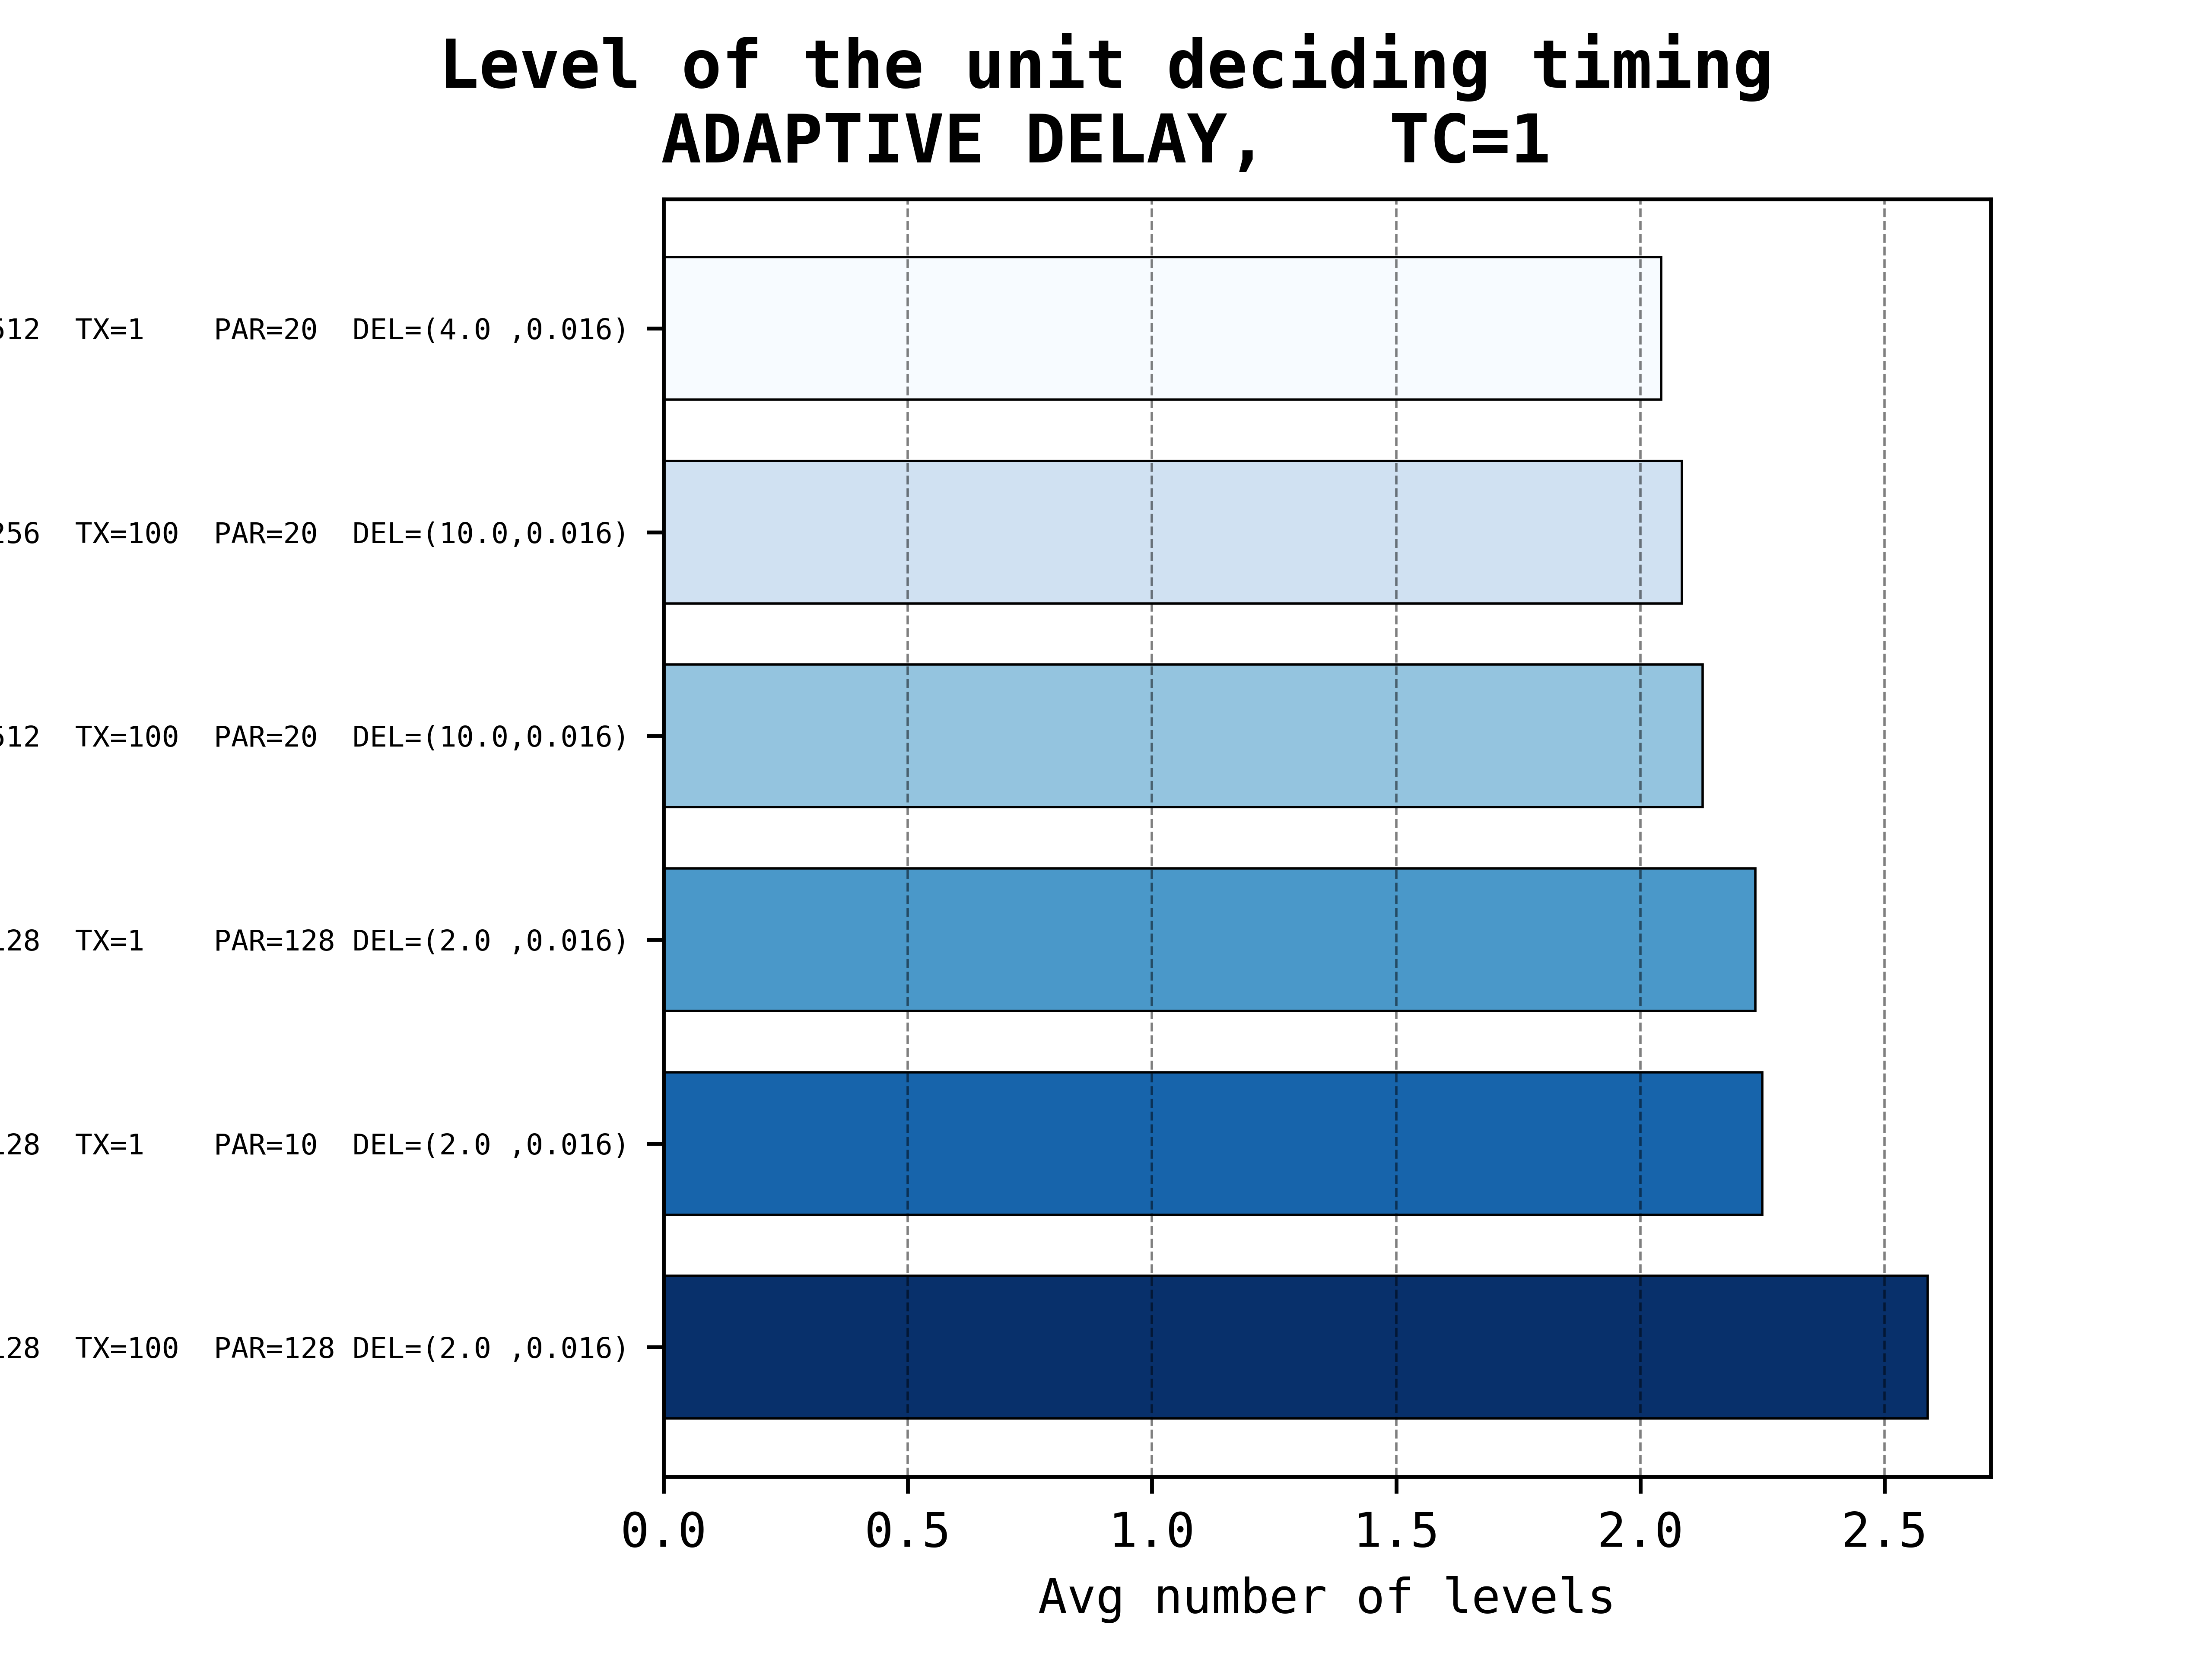
\includegraphics[width=0.8\textwidth]{bar_plots/big/decision_height.png}
				\caption{How many levels above the considered unit was the timing decision taken, on average.}
				\label{fig:bigDecisionUnit}
			\end{figure}
			\begin{figure}[h]
				\centering
				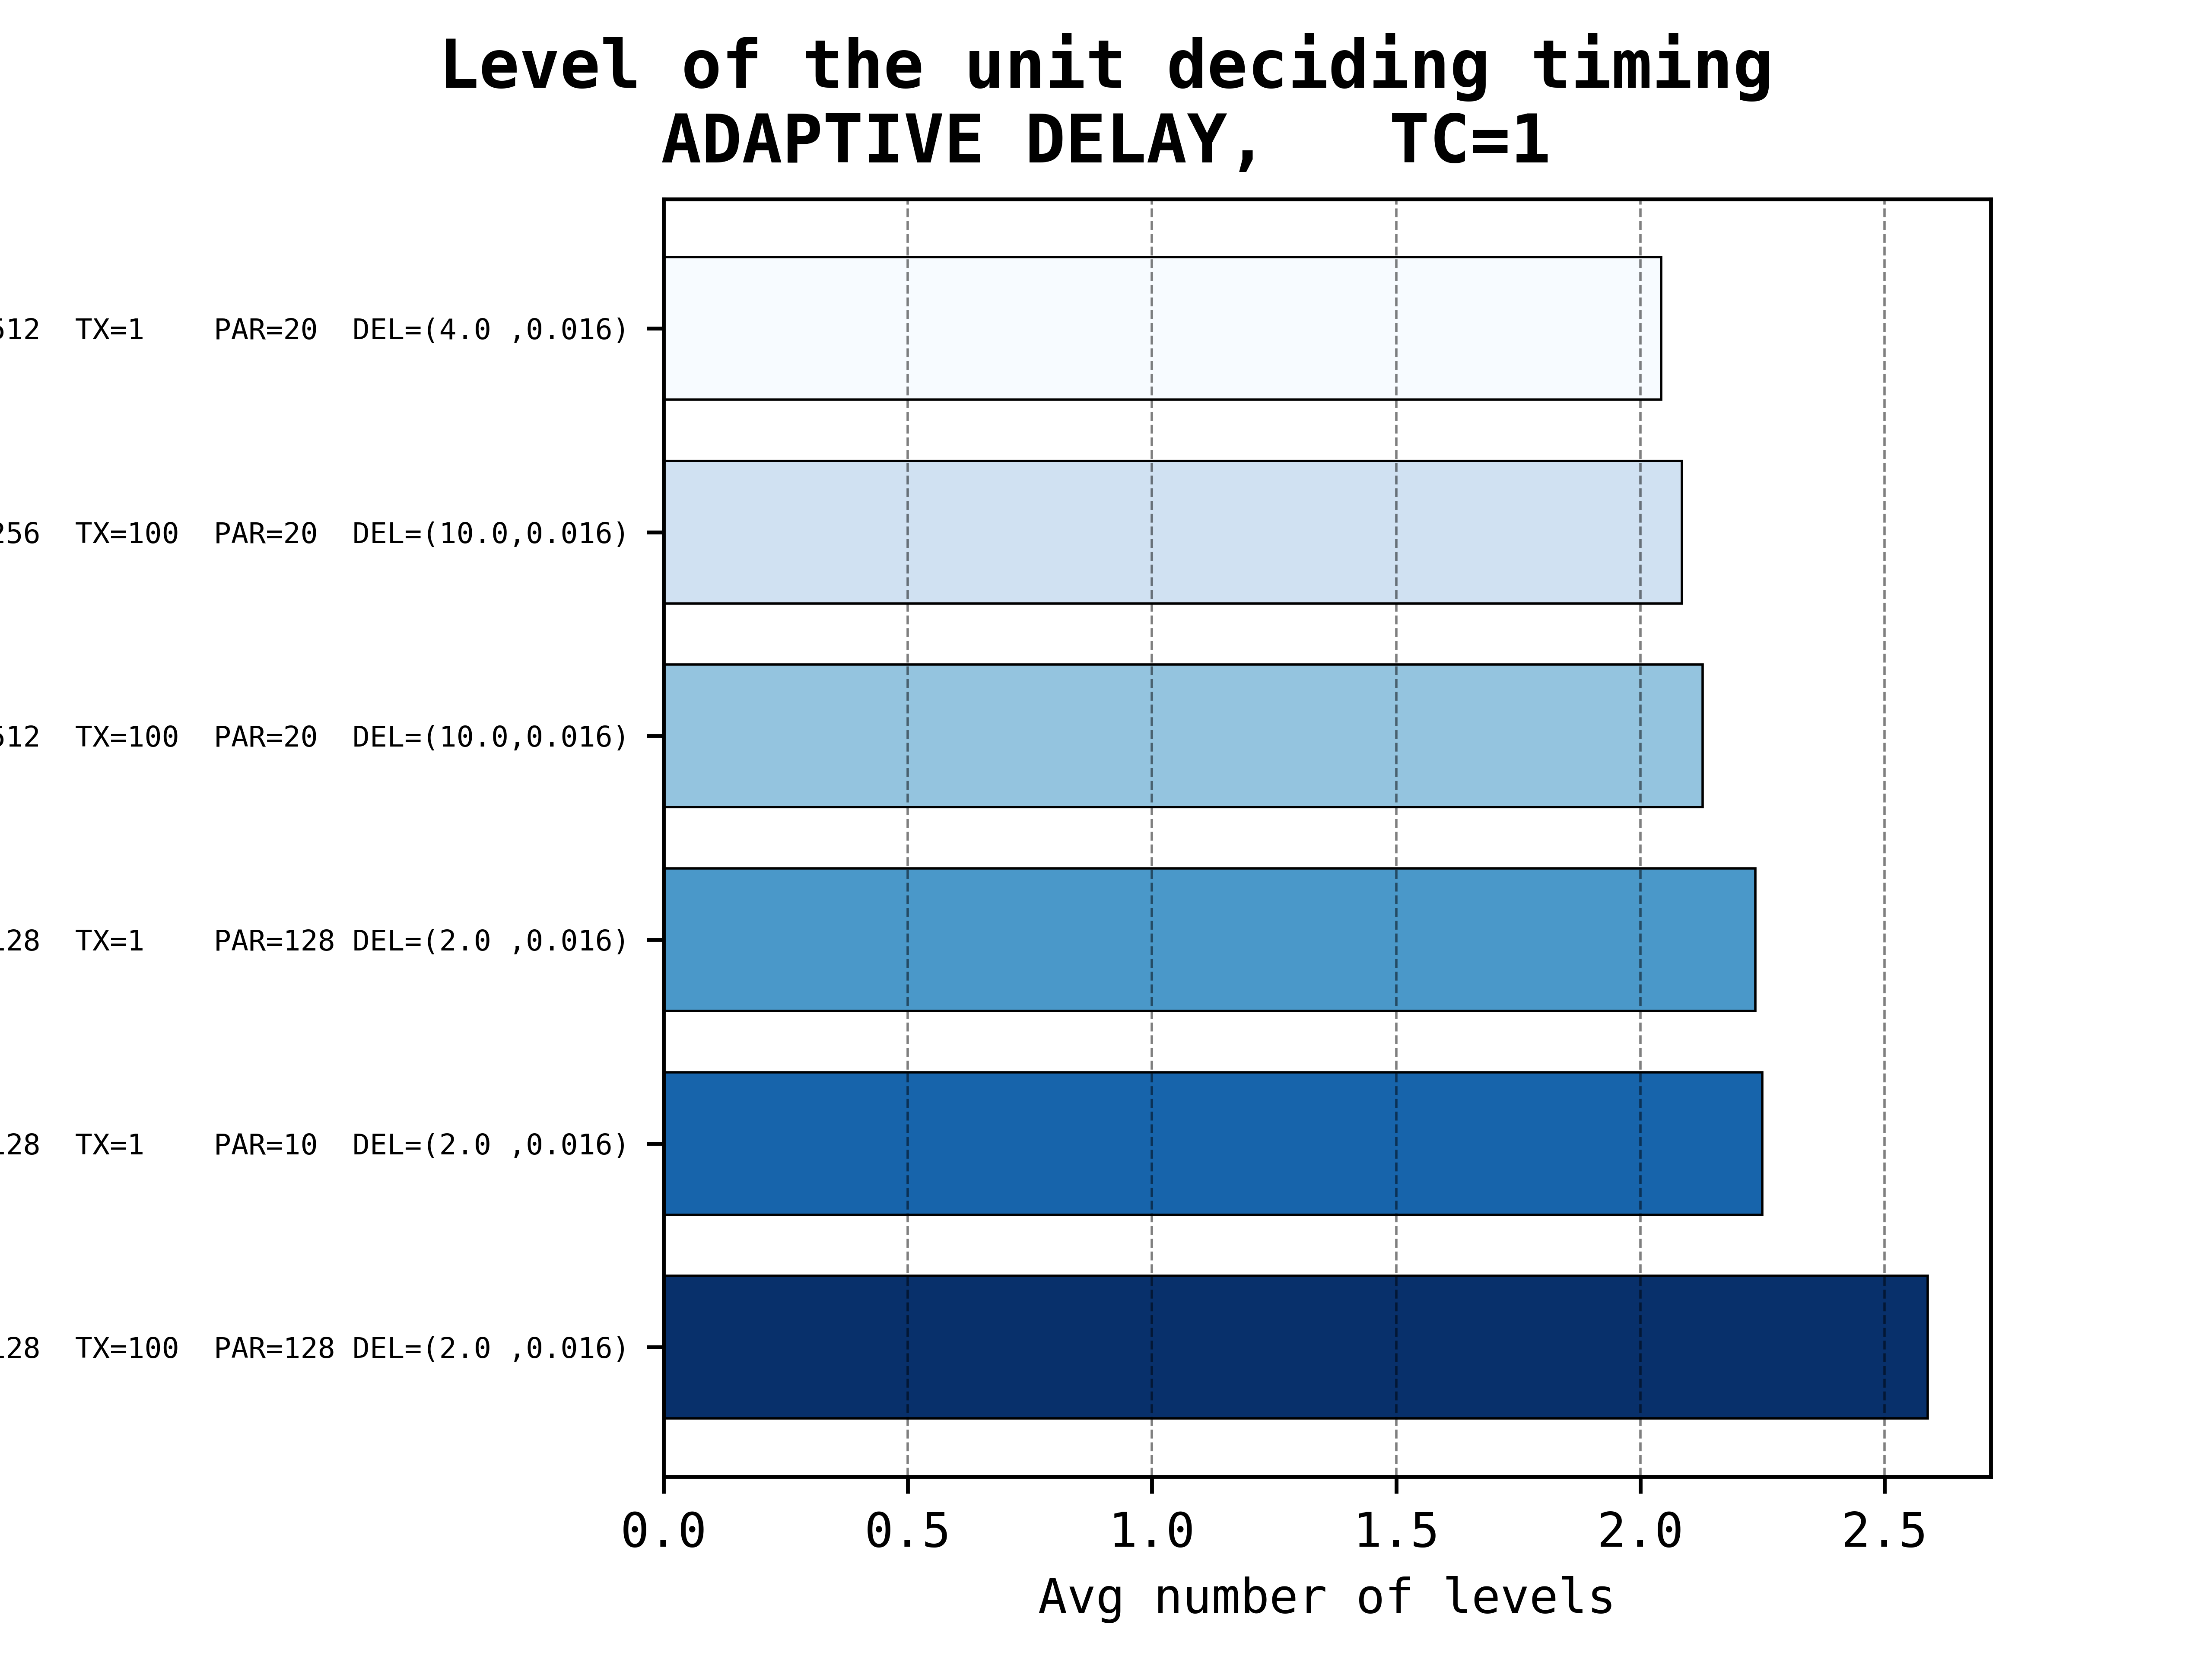
\includegraphics[width=0.8\textwidth]{bar_plots/big/decision_height.png}
				\caption{How many levels above the considered unit was the maximal unit in the poset when the timing decision was made, on average. Compare with Figure \ref{fig:bigDecisionUnit}.}
				\label{fig:bigDecisionPoset}
			\end{figure}
			\begin{figure}[h]
				\centering
				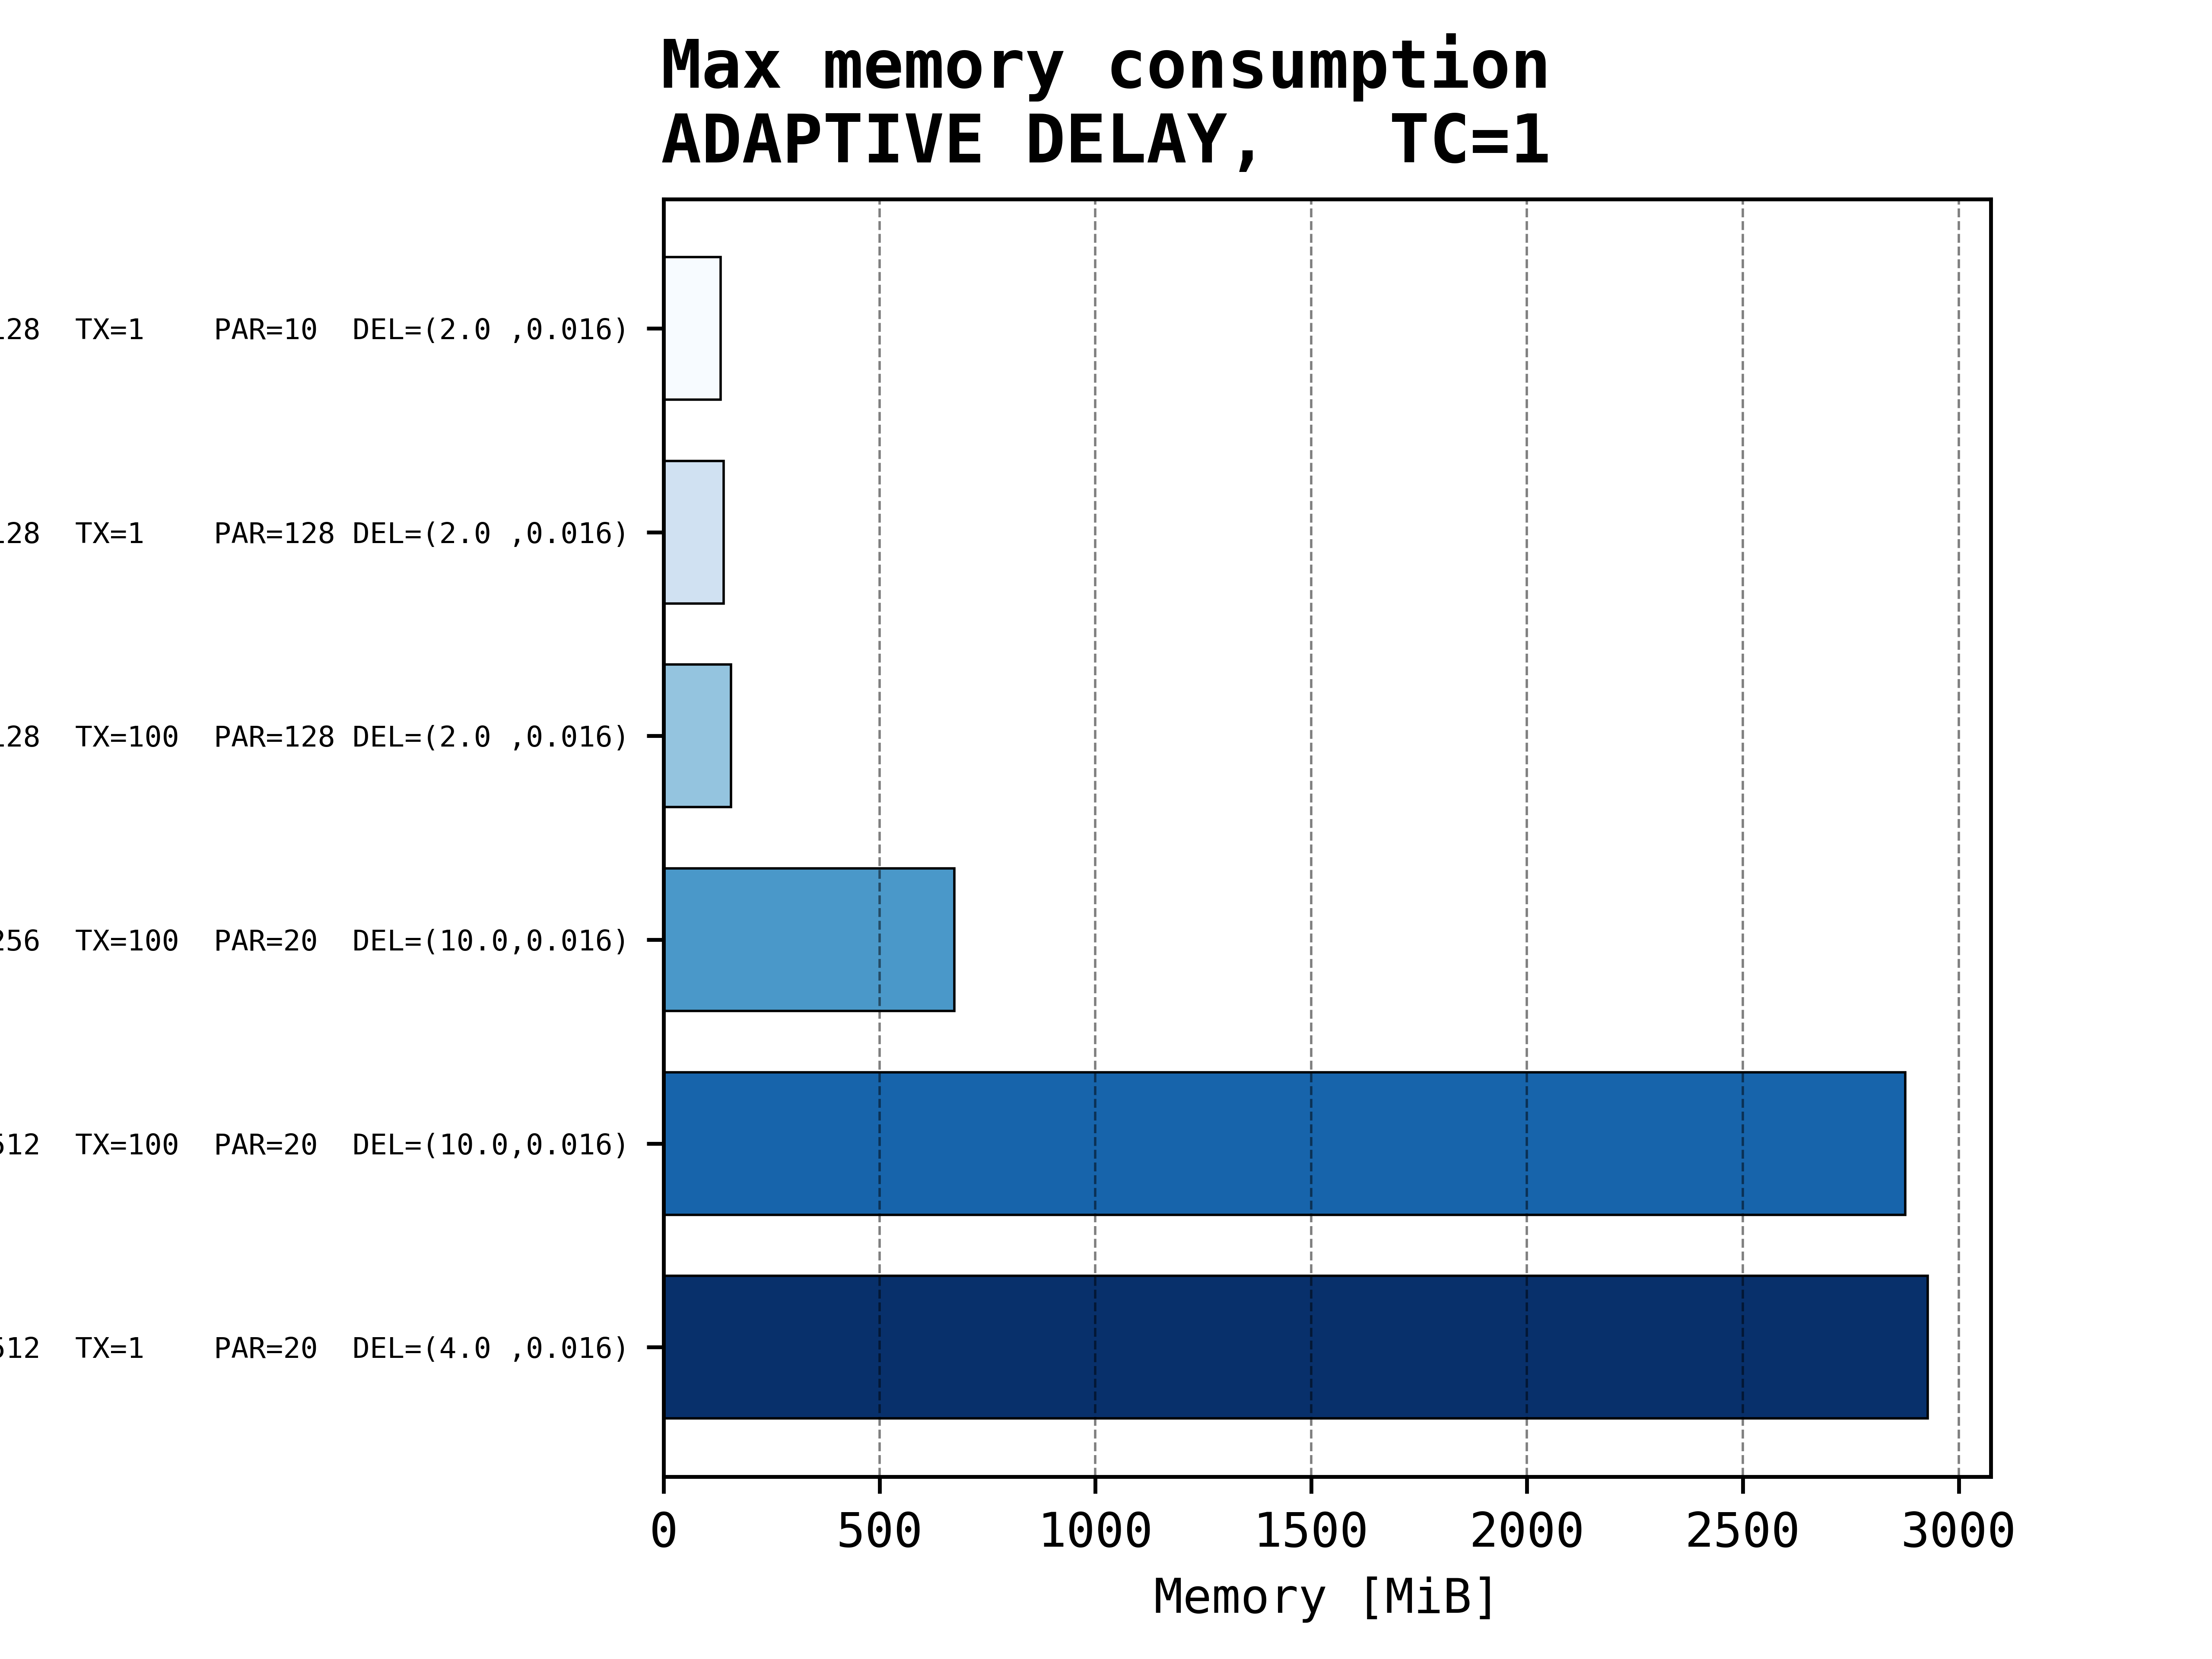
\includegraphics[width=0.8\textwidth]{bar_plots/big/memory_MiB.png}
				\caption{The amount of RAM used by a process. Note that this is for $50$ levels.}
				\label{fig:bigRAM}
			\end{figure}
			\begin{figure}[h]
				\centering
				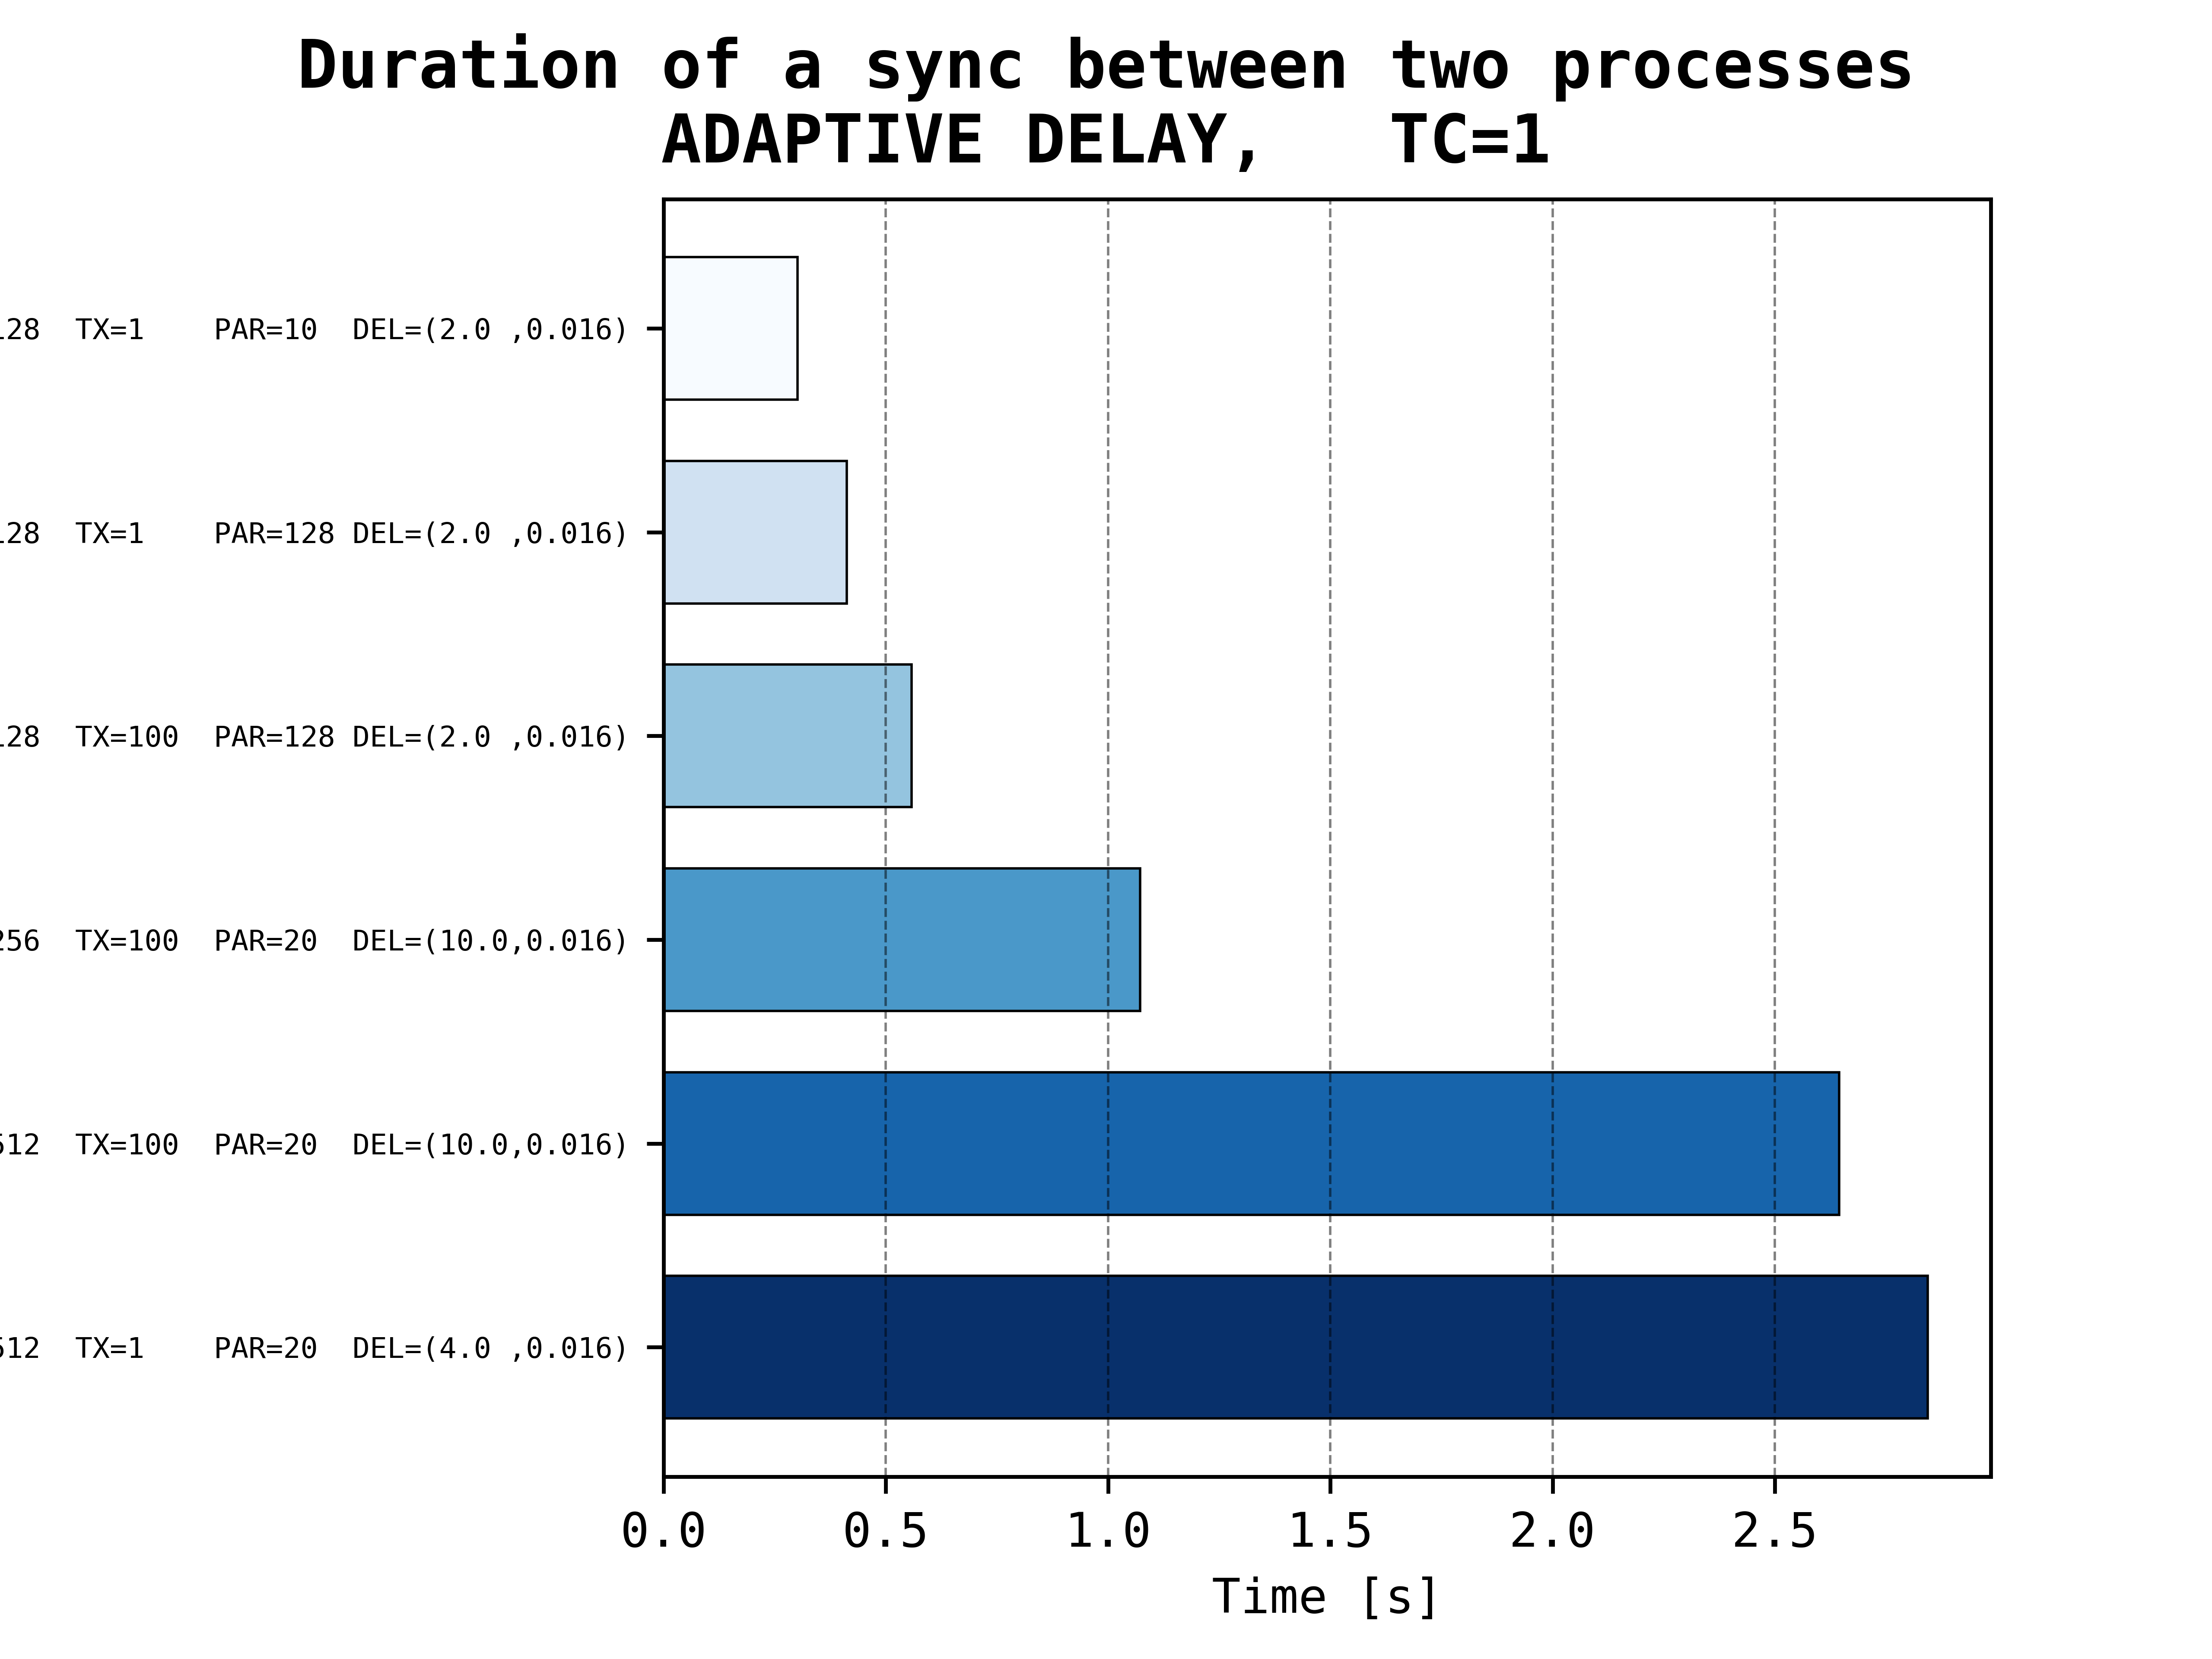
\includegraphics[width=0.8\textwidth]{bar_plots/big/time_per_sync.png}
				\caption{The average time a single sync operation took.}
				\label{fig:bigTimePerSync}
			\end{figure}
			\begin{figure}[h]
				\centering
				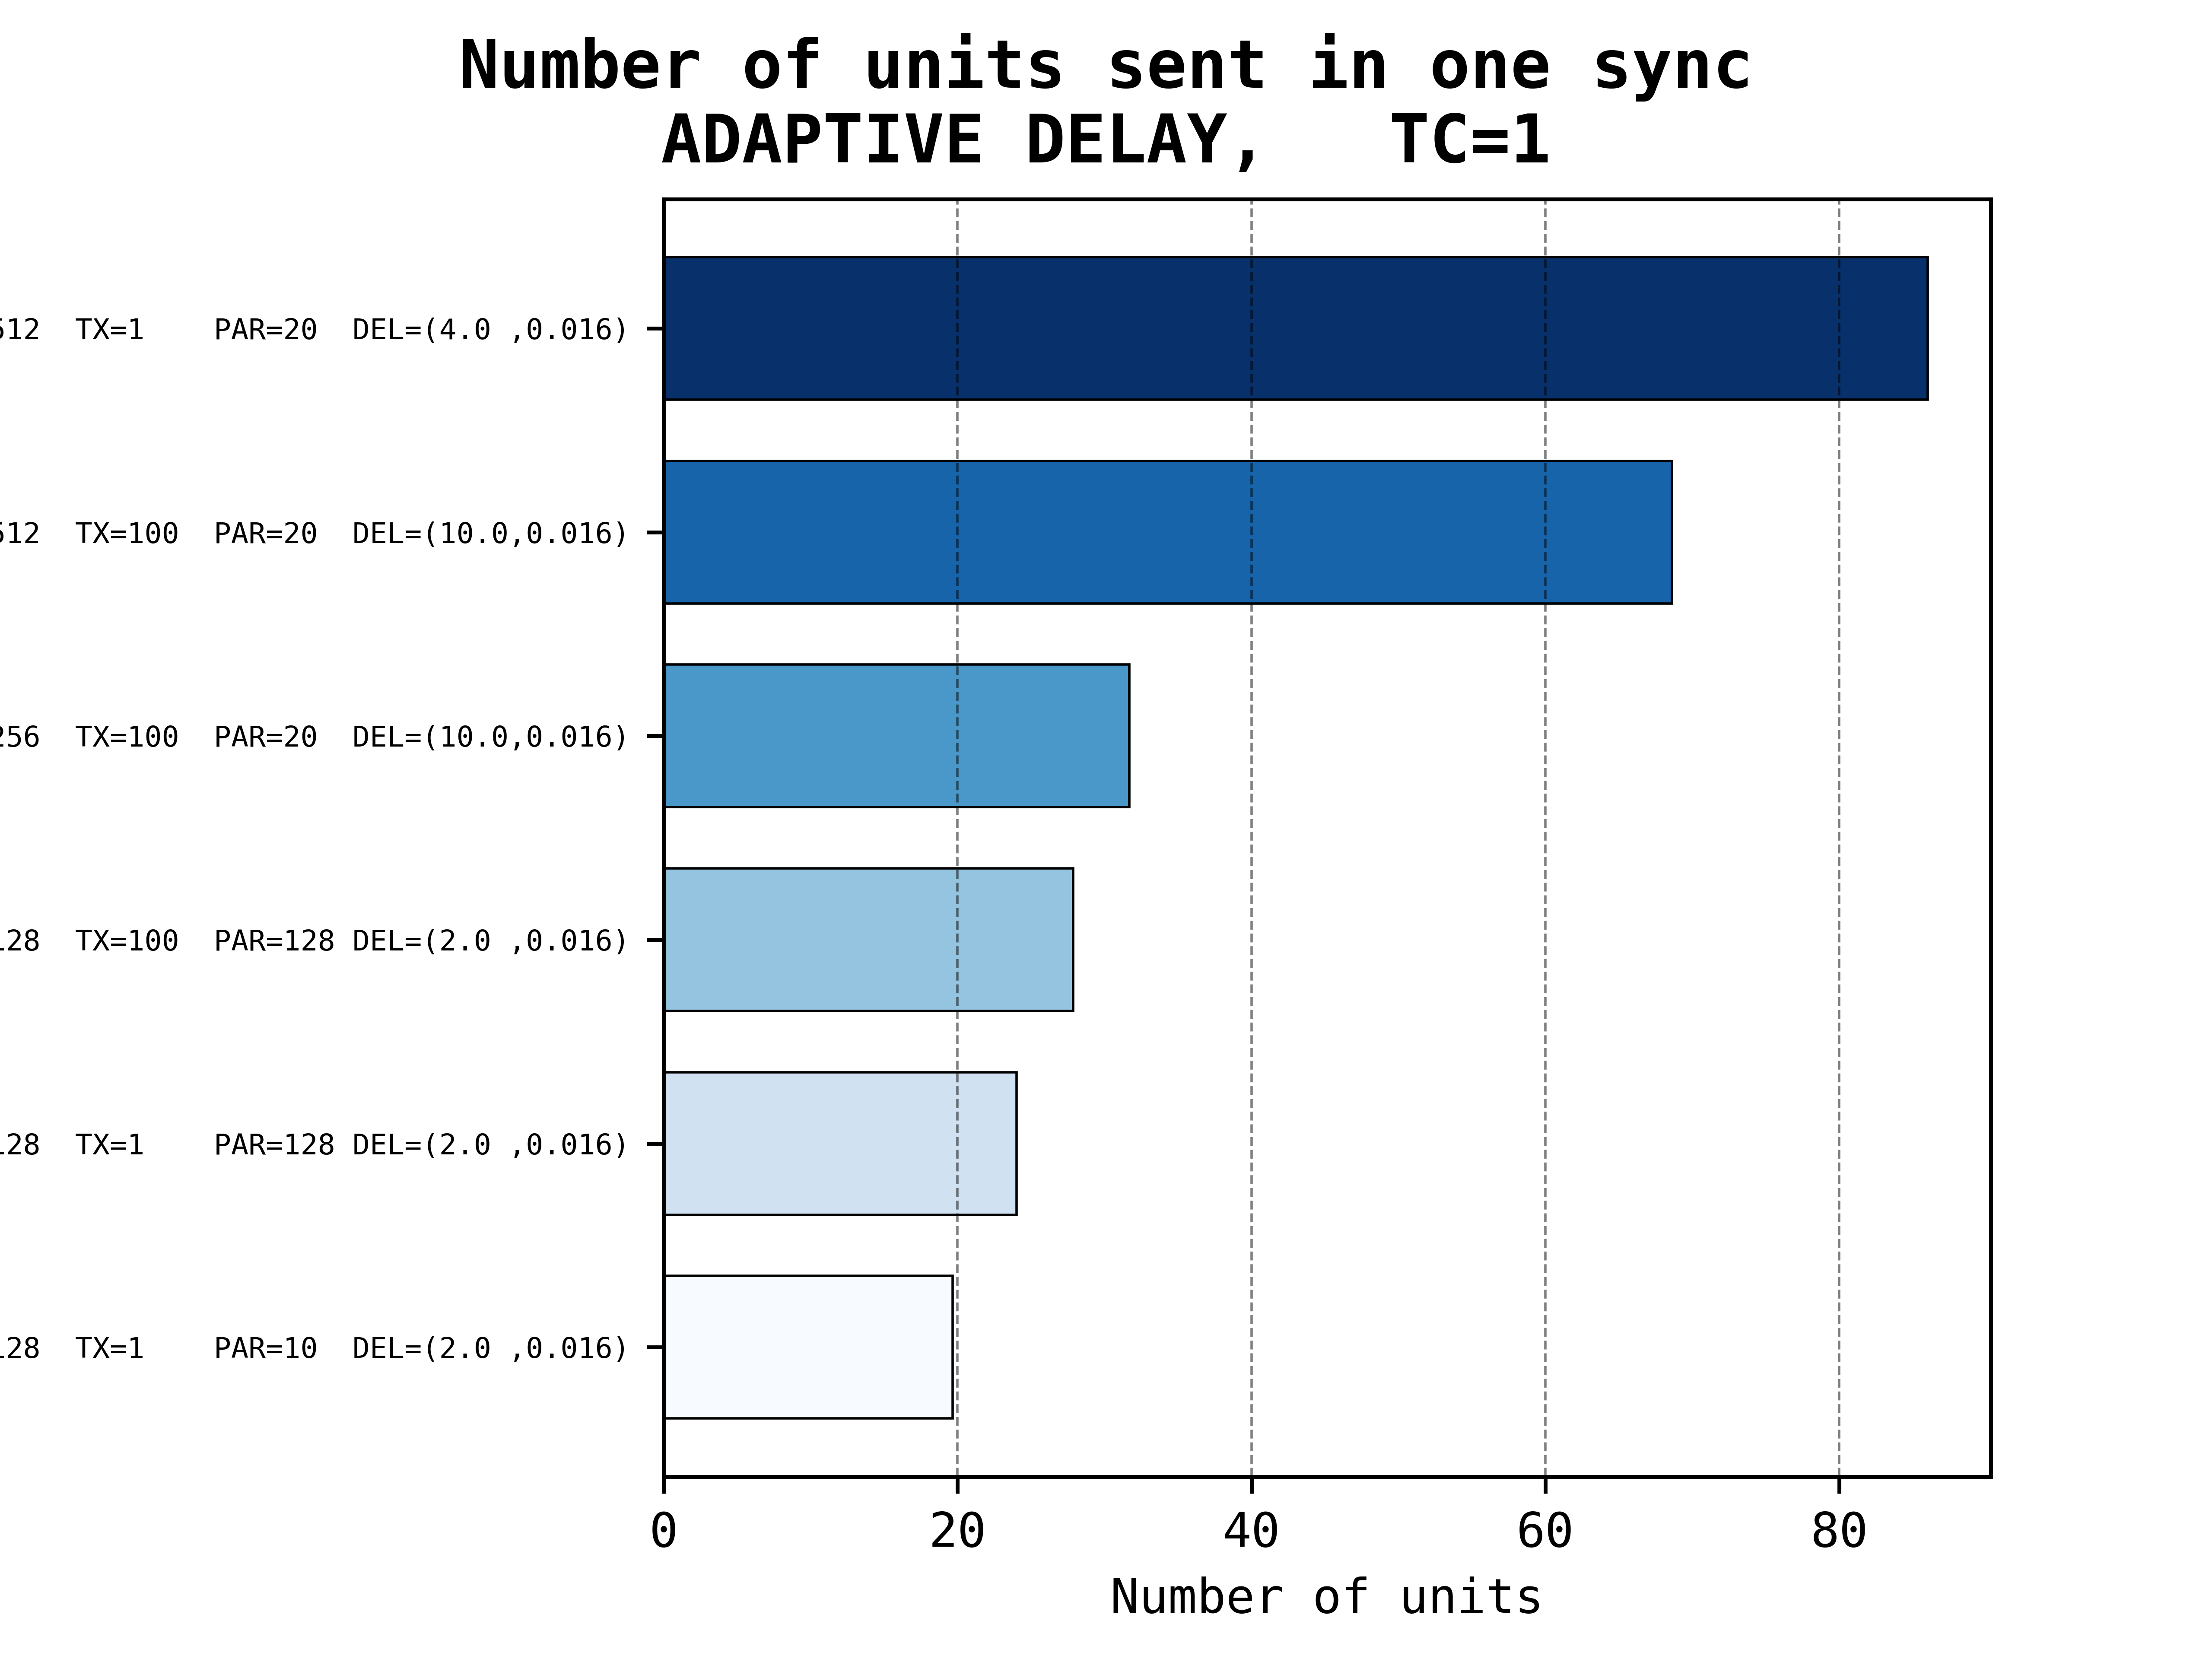
\includegraphics[width=0.8\textwidth]{bar_plots/big/units_sent_sync.png}
				\caption{The average number of units sent per sync.}
				\label{fig:bigUnitsPerSync}
			\end{figure}
			\begin{figure}[h]
				\centering
				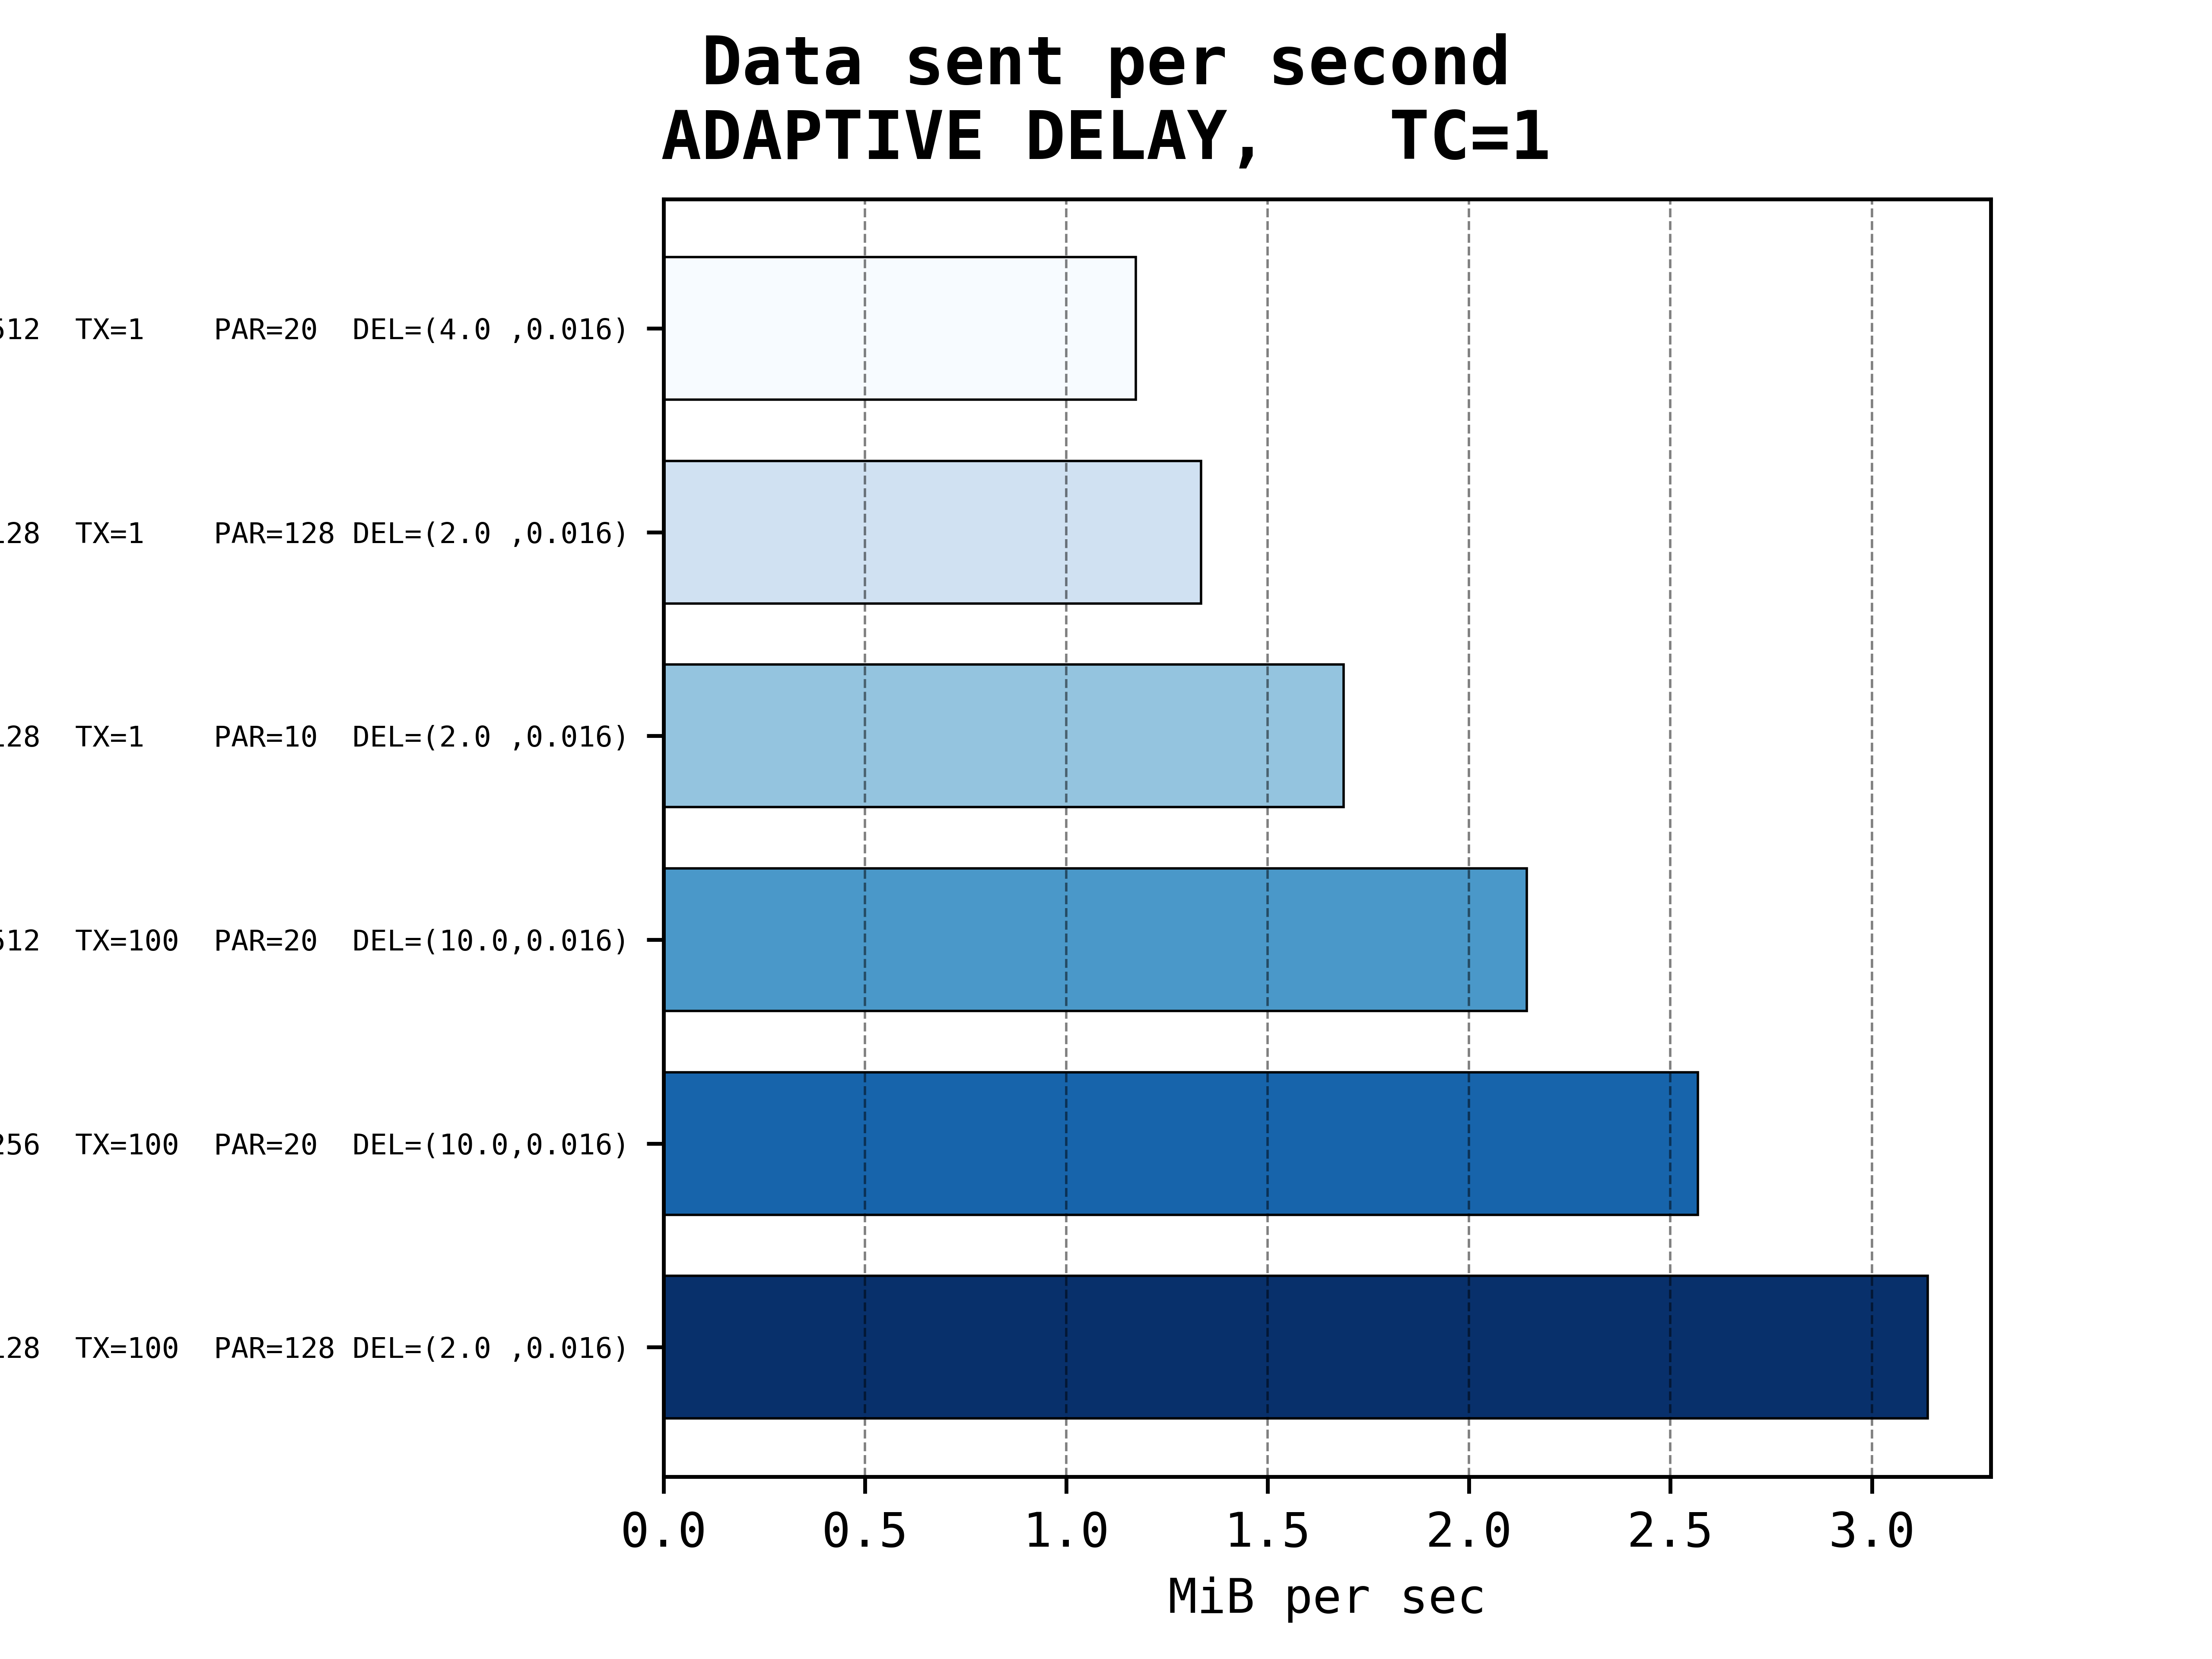
\includegraphics[width=0.8\textwidth]{bar_plots/big/bytes_sent_per_sec.png}
				\caption{The average amount of data sent per second.}
				\label{fig:bigBps}
			\end{figure}
\end{document}
